\begin{minipage}[b]{0.33\linewidth}
\begin{lrbox}{\mybox}%
\begin{lstlisting}[basicstyle=\ttfamily\tiny,escapechar=\%]
* = $0801
;---------------------------------
; Start program at InitializeProgram%\index{InitializeProgram}%
; SYS 2064 ($0810)
;---------------------------------
 .BYTE $0B,$08
 .BYTE $C1,$07
 .BYTE $9E
 .BYTE $32,$30,$36,$34
 .BYTE $00
 .BYTE $00,$00
 .BYTE $F9,$02,$F9


;------------------------------
; InitializeProgram%\index{InitializeProgram}%
;------------------------------
InitializeProgram%\index{InitializeProgram}%
 LDA #$00
 STA $D020
 STA $D021

 JSR MovePresetDataIntoPosition%\index{MovePresetDataIntoPosition}%

 STA previousIndexToPixelBuffers%\index{previousIndexToPixelBuffers}%

 LDA #>COLOR_RAM
 STA colorRamHiPtr%\index{colorRamHiPtr}%
 LDA #<COLOR_RAM
 STA colorRamLoPtr%\index{colorRamLoPtr}%

 LDX #$00
InitColorRamTableLoop
 LDA colorRamHiPtr%\index{colorRamHiPtr}%
 STA colorRAMLineTableHiPtrArray%\index{colorRAMLineTableHiPtrArray}%,X
 LDA colorRamLoPtr%\index{colorRamLoPtr}%
 STA colorRAMLineTableLoPtrArray%\index{colorRAMLineTableLoPtrArray}%,X
 CLC
 ADC #NUM_COLS
 STA colorRamLoPtr%\index{colorRamLoPtr}%
 LDA colorRamHiPtr%\index{colorRamHiPtr}%
 ADC #$00
 STA colorRamHiPtr%\index{colorRamHiPtr}%
 INX
 CPX #NUM_ROWS + 1
 BNE InitColorRamTableLoop

 LDA #$80
 STA $0291

 LDA #$15
 STA $D018

 JSR ROM_IOINIT
 JSR InitializeDynamicStorage%\index{InitializeDynamicStorage}%
 JMP LaunchPsychedelia%\index{LaunchPsychedelia}%

colorRAMLineTableLoPtrArray%\index{colorRAMLineTableLoPtrArray}%
 .BYTE $00,$00,$00,$00,$00,$00,$00,$00
 .BYTE $00,$00,$00,$00,$00,$00,$00,$00
 .BYTE $00,$00,$00,$00,$00,$00,$00,$00
 .BYTE $00,$00,$00,$00,$00,$00
colorRAMLineTableHiPtrArray%\index{colorRAMLineTableHiPtrArray}%
 .BYTE $00,$00,$00,$00,$00,$00,$BF,$00
 .BYTE $00,$00,$00,$00,$00,$00,$00,$00
 .BYTE $00,$00,$00,$00,$00,$00,$00,$00
 .BYTE $00,$00,$00,$00,$00,$00

;------------------------------
; InitializeScreenWithInitCharacter%\index{InitializeScreenWithInitCharacter}%
;------------------------------
InitializeScreenWithInitCharacter%\index{InitializeScreenWithInitCharacter}%
 LDX #$00

currentPixel = *+$01
InitScreenLoop
 LDA #$CF
 STA SCREEN_RAM + $0000,X
 STA SCREEN_RAM + $0100,X
 STA SCREEN_RAM + $0200,X
 STA SCREEN_RAM + $02C0,X
 LDA #$00
 STA COLOR_RAM + $0000,X
 STA COLOR_RAM + $0100,X
 STA COLOR_RAM + $0200,X
 STA COLOR_RAM + $02C0,X
 DEX
 BNE InitScreenLoop
 RTS

presetKeyCodes
 .BYTE KEY_LEFT,KEY_1,KEY_2,KEY_3
 .BYTE KEY_4,KEY_5,KEY_6,KEY_7
 .BYTE KEY_8,KEY_9,KEY_0,KEY_PLUS
 .BYTE KEY_MINUS,KEY_POUND
 .BYTE KEY_CLR_HOME,KEY_INST_DEL

;------------------------------
; LoadXAndYPosition%\index{LoadXAndYPosition}%
;------------------------------
LoadXAndYPosition%\index{LoadXAndYPosition}%
 LDX pixelYPosition%\index{pixelYPosition}%
 LDA colorRAMLineTableLoPtrArray%\index{colorRAMLineTableLoPtrArray}%,X
 STA currentLineInColorRamLoPtr2
 LDA colorRAMLineTableHiPtrArray%\index{colorRAMLineTableHiPtrArray}%,X
 STA currentLineInColorRamHiPtr2
 LDY pixelXPosition%\index{pixelXPosition}%
ReturnEarlyFromRoutine%\index{ReturnEarlyFromRoutine}%
 RTS
\end{lstlisting}
\end{lrbox}%
\scalebox{0.8}{\usebox{\mybox}}
\end{minipage}
\hspace{-0.1cm}
\begin{minipage}[b]{0.33\linewidth}
\begin{lrbox}{\mybox}%
\begin{lstlisting}[basicstyle=\ttfamily\tiny,escapechar=\%]
;------------------------------
; PaintPixel%\index{PaintPixel}%
;------------------------------
PaintPixel%\index{PaintPixel}%
 LDA pixelXPosition%\index{pixelXPosition}%
 AND #$80
 BNE ReturnEarlyFromRoutine%\index{ReturnEarlyFromRoutine}%
 LDA pixelXPosition%\index{pixelXPosition}%
 CMP #NUM_COLS
 BPL ReturnEarlyFromRoutine%\index{ReturnEarlyFromRoutine}%
 LDA pixelYPosition%\index{pixelYPosition}%
 AND #$80
 BNE ReturnEarlyFromRoutine%\index{ReturnEarlyFromRoutine}%
 LDA pixelYPosition%\index{pixelYPosition}%
 CMP #NUM_ROWS
 BPL ReturnEarlyFromRoutine%\index{ReturnEarlyFromRoutine}%

 JSR LoadXAndYPosition%\index{LoadXAndYPosition}%
 LDA skipPixel%\index{skipPixel}%
 BNE ActuallyPaintPixel%\index{ActuallyPaintPixel}%

 LDA (currentLineInColorRamLoPtr2),Y
 AND #COLOR_MAX

 LDX #$00
GetIndexInPresetsLoop
 CMP presetColorValuesArray%\index{presetColorValuesArray}%,X
 BEQ FoundMatchingIndex
 INX
 CPX #COLOR_VALUES_ARRAY_LEN
 BNE GetIndexInPresetsLoop

FoundMatchingIndex
 TXA
 STA indexOfCurrentColor%\index{indexOfCurrentColor}%
 LDX currentValueInColorIndexArray%\index{currentValueInColorIndexArray}%
 INX
 CPX indexOfCurrentColor%\index{indexOfCurrentColor}%
 BEQ ActuallyPaintPixel%\index{ActuallyPaintPixel}%
 BPL ActuallyPaintPixel%\index{ActuallyPaintPixel}%
 RTS

ActuallyPaintPixel%\index{ActuallyPaintPixel}%
 LDX currentValueInColorIndexArray%\index{currentValueInColorIndexArray}%
 LDA presetColorValuesArray%\index{presetColorValuesArray}%,X
 STA (currentLineInColorRamLoPtr2),Y
 RTS

;------------------------------
; PaintStructureAtCurrentPosition%\index{PaintStructureAtCurrentPosition}%
;------------------------------
PaintStructureAtCurrentPosition%\index{PaintStructureAtCurrentPosition}%
 JSR PaintPixelForCurrentSymmetry%\index{PaintPixelForCurrentSymmetry}%
 LDY #$00
 LDA currentValueInColorIndexArray%\index{currentValueInColorIndexArray}%
 CMP #NUM_ARRAYS
 BNE CanLoopAndPaint
 RTS

CanLoopAndPaint
 LDA #NUM_ARRAYS
 STA countToMatchCurrentIndex%\index{countToMatchCurrentIndex}%

 LDA pixelXPosition%\index{pixelXPosition}%
 STA previousPixelXPosition%\index{previousPixelXPosition}%
 LDA pixelYPosition%\index{pixelYPosition}%
 STA previousPixelYPosition%\index{previousPixelYPosition}%

 LDX patternIndex%\index{patternIndex}%
 LDA pixelXPositionLoPtrArray,X
 STA xPosLoPtr
 LDA pixelXPositionHiPtrArray,X
 STA xPosHiPtr
 LDA pixelYPositionLoPtrArray,X
 STA yPosLoPtr
 LDA pixelYPositionHiPtrArray,X
 STA yPosHiPtr

PixelPaintLoop%\index{PixelPaintLoop}%
 LDA previousPixelXPosition%\index{previousPixelXPosition}%
 CLC
 ADC (xPosLoPtr),Y
 STA pixelXPosition%\index{pixelXPosition}%
 LDA previousPixelYPosition%\index{previousPixelYPosition}%
 CLC
 ADC (yPosLoPtr),Y
 STA pixelYPosition%\index{pixelYPosition}%

 TYA
 PHA
 JSR PaintPixelForCurrentSymmetry%\index{PaintPixelForCurrentSymmetry}%
 PLA
 TAY
 INY

 LDA (xPosLoPtr),Y
 CMP #$55
 BNE PixelPaintLoop%\index{PixelPaintLoop}%

 DEC countToMatchCurrentIndex%\index{countToMatchCurrentIndex}%
 LDA countToMatchCurrentIndex%\index{countToMatchCurrentIndex}%
 CMP currentValueInColorIndexArray%\index{currentValueInColorIndexArray}%
 BEQ RestorePositionsAndReturn%\index{RestorePositionsAndReturn}%

 CMP #$01
 BEQ RestorePositionsAndReturn%\index{RestorePositionsAndReturn}%

 INY
 JMP PixelPaintLoop%\index{PixelPaintLoop}%
\end{lstlisting}
\end{lrbox}%
\scalebox{0.8}{\usebox{\mybox}}
\end{minipage}
\hspace{-0.1cm}
\begin{minipage}[b]{0.33\linewidth}
\begin{lrbox}{\mybox}%
\begin{lstlisting}[basicstyle=\ttfamily\tiny,escapechar=\%]
RestorePositionsAndReturn%\index{RestorePositionsAndReturn}%
 LDA previousPixelXPosition%\index{previousPixelXPosition}%
 STA pixelXPosition%\index{pixelXPosition}%
 LDA previousPixelYPosition%\index{previousPixelYPosition}%
 STA pixelYPosition%\index{pixelYPosition}%
 RTS

;        5       
;                
;       4 4      
;        3       
;        2       
;        1       
;   4   000   4  
; 5  3210 0123  5
;   4   000   4  
;        1       
;        2       
;        3       
;       4 4      
;                
;        5       
starOneXPosArray%\index{starOneXPosArray}%  
.BYTE $00,$01,$01,$01,$00
.BYTE $FF,$FF,$FF,$55
.BYTE $00,$02,$00,$FE,$55
.BYTE $00,$03,$00,$FD,$55
.BYTE $00,$04,$00,$FC,$55
.BYTE $FF,$01,$05,$05,$01
.BYTE $FF,$FB,$FB,$55
.BYTE $00,$07,$00,$F9,$55
.BYTE $55
starOneYPosArray%\index{starOneYPosArray}%  
.BYTE $FF,$FF,$00,$01,$01
.BYTE $01,$00,$FF,$55
.BYTE $FE,$00,$02,$00,$55
.BYTE $FD,$00,$03,$00,$55
.BYTE $FC,$00,$04,$00,$55
.BYTE $FB,$FB,$FF,$01,$05
.BYTE $05,$01,$FF,$55
.BYTE $F9,$00,$07,$00,$55
.BYTE $55

countToMatchCurrentIndex%\index{countToMatchCurrentIndex}%   .BYTE $00

;------------------------------
; PutRandomByteInAccumulator%\index{PutRandomByteInAccumulator}%
;------------------------------
PutRandomByteInAccumulator%\index{PutRandomByteInAccumulator}%
randomByteAddress   =*+$01
 LDA $E199,X
 INC randomByteAddress
 RTS

;------------------------------
; PaintPixelForCurrentSymmetry%\index{PaintPixelForCurrentSymmetry}%
;------------------------------
PaintPixelForCurrentSymmetry%\index{PaintPixelForCurrentSymmetry}%
 LDA pixelXPosition%\index{pixelXPosition}%
 PHA
 LDA pixelYPosition%\index{pixelYPosition}%
 PHA
 JSR PaintPixel%\index{PaintPixel}%

 LDA currentSymmetrySettingForStep%\index{currentSymmetrySettingForStep}%
 BNE HasSymmetry

CleanUpAndReturnFromSymmetry
 PLA
 STA pixelYPosition%\index{pixelYPosition}%
 PLA
 STA pixelXPosition%\index{pixelXPosition}%
 RTS

HasSymmetry
 CMP #X_AXIS_SYMMETRY
 BEQ XAxisSymmetry

 LDA #NUM_COLS - 1
 SEC
 SBC pixelXPosition%\index{pixelXPosition}%
 STA pixelXPosition%\index{pixelXPosition}%

 LDY currentSymmetrySettingForStep%\index{currentSymmetrySettingForStep}%
 CPY #X_Y_SYMMETRY
 BEQ XYSymmetry

 JSR PaintPixel%\index{PaintPixel}%

 LDA currentSymmetrySettingForStep%\index{currentSymmetrySettingForStep}%
 CMP #Y_AXIS_SYMMETRY
 BEQ CleanUpAndReturnFromSymmetry

 LDA #NUM_ROWS - 1
 SEC
 SBC pixelYPosition%\index{pixelYPosition}%
 STA pixelYPosition%\index{pixelYPosition}%
 JSR PaintPixel%\index{PaintPixel}%

PaintXAxisPixelForSymmetry
 PLA
 TAY
 PLA
 STA pixelXPosition%\index{pixelXPosition}%
 TYA
 PHA
 JSR PaintPixel%\index{PaintPixel}%
 PLA
 STA pixelYPosition%\index{pixelYPosition}%
 RTS

\end{lstlisting}
\end{lrbox}%
\scalebox{0.8}{\usebox{\mybox}}
\end{minipage}
\clearpage
\rhead[]{The Core of the Game on a Page or Two}
\textbf{Lines 1 - 710.} This first section is almost exactly the same as its equivalent in the listing. On this
page and the following two we have the core of the game from which the version we saw in 
\hyperref[sec:commentary]{\textcolor{blue}{'let's pretend we can read code'}} was carved out.

What this tells us, I think, is that what we have here and in the following two pages represents the very initial state
of Psychedelia when it was first developed: 

\begin{definition}[Jeffrey Says\index{Jeffrey Says}]
\setlength{\intextsep}{0pt}%
\setlength{\columnsep}{3pt}%
\begin{wrapfigure}{l}{0.12\textwidth}

\includegraphics[width=\linewidth]{src/callout/psych.png} 
\end{wrapfigure}
\small
.. one day I was out running and an just appeared unbidden in my head. I still
  remember the exact bit of road I was on when it happened. It was a
  simple algorithm, just seeding patterns along a path; the patterns were to
  expand and change shape and colour over time. I got back from my run and
  coded up the algo - it fit in about 1K of 6502 assembler code. I ran the code
  and a white cursor appeared on the screen. i picked up the joystick, moved
  the cursor, and pressed down the fire button.

In that instant my life changed.
\end{definition}

So this three pages of code is the product of an evening's work - the nucleus of the game as a whole. The fact that among
the code we have a single data structure for a single pattern reinforces this notion: a simple demo neededed just one
pattern to work with, so there it is, propped between \icode{PaintStructureAtCurrentPosition\index{PaintStructureAtCurrentPosition}} and \icode{PaintPixelForCurrentSymmetry\index{PaintPixelForCurrentSymmetry}}.

Once the basic demo was working, it was time to add some more patterns and we can see these inserted after the interrupt handler
code in the final column on the following pages: 'The Twist', 'La Llamita', and 'Star Two' make their appearance.

The writing of a complete game was underway.

\clearpage
\begin{minipage}[b]{0.33\linewidth}
\begin{lrbox}{\mybox}%
\begin{lstlisting}[basicstyle=\ttfamily\tiny,escapechar=\%]
XAxisSymmetry
 LDA #NUM_ROWS - 1
 SEC
 SBC pixelYPosition%\index{pixelYPosition}%
 STA pixelYPosition%\index{pixelYPosition}%
 JMP PaintXAxisPixelForSymmetry
XYSymmetry
 LDA #NUM_ROWS - 1
 SEC
 SBC pixelYPosition%\index{pixelYPosition}%
 STA pixelYPosition%\index{pixelYPosition}%
 JSR PaintPixel%\index{PaintPixel}%
 PLA
 STA pixelYPosition%\index{pixelYPosition}%
 PLA
 STA pixelXPosition%\index{pixelXPosition}%
 RTS

pixelXPositionArray%\index{pixelXPositionArray}%
 .BYTE $00,$00,$FF,$00,$00,$00,$00,$00
 .BYTE $00,$00,$00,$00,$00,$00,$00,$00
 .BYTE $00,$00,$00,$00,$00,$00,$00,$00
 .BYTE $00,$00,$FF,$00,$00,$00,$00,$00
 .BYTE $00,$00,$00,$00,$00,$00,$00,$00
 .BYTE $00,$00,$00,$00,$00,$00,$00,$00
 .BYTE $00,$00,$00,$00,$00,$00,$00,$00
 .BYTE $00,$00,$00,$00,$00,$00,$00,$00
pixelYPositionArray%\index{pixelYPositionArray}%
 .BYTE $00,$00,$FD,$00,$00,$00,$00,$00
 .BYTE $00,$00,$00,$00,$00,$00,$00,$00
 .BYTE $00,$00,$00,$00,$00,$00,$00,$00
 .BYTE $00,$00,$00,$00,$00,$00,$00,$00
 .BYTE $00,$00,$00,$00,$00,$00,$00,$00
 .BYTE $00,$00,$00,$00,$00,$00,$00,$00
 .BYTE $00,$00,$00,$00,$00,$00,$00,$00
 .BYTE $00,$00,$00,$00,$00,$00,$00,$00
currentColorIndexArray%\index{currentColorIndexArray}%
 .BYTE $00,$00,$00,$00,$00,$00,$00,$00
 .BYTE $00,$00,$00,$00,$00,$00,$00,$00
 .BYTE $00,$00,$00,$00,$00,$00,$00,$00
 .BYTE $00,$00,$00,$00,$00,$00,$00,$00
 .BYTE $00,$00,$00,$00,$00,$00,$00,$00
 .BYTE $00,$00,$00,$00,$00,$00,$00,$00
 .BYTE $00,$00,$00,$00,$00,$00,$00,$00
 .BYTE $00,$00,$00,$00,$00,$00,$00,$00
initialSmoothingDelayArray%\index{initialSmoothingDelayArray}%
 .BYTE $00,$00,$00,$00,$00,$00,$00,$00
 .BYTE $00,$00,$00,$00,$00,$00,$00,$00
 .BYTE $00,$00,$00,$00,$00,$00,$00,$00
 .BYTE $00,$00,$FF,$FF,$FF,$FF,$FF,$FF
 .BYTE $FF,$FF,$FF,$FF,$FF,$FF,$FF,$FF
 .BYTE $FF,$FF,$FF,$FF,$FF,$FF,$FF,$FF
 .BYTE $FF,$FF,$FF,$FF,$FF,$FF,$FF,$FF
 .BYTE $FF,$FF,$FF,$FF,$FF,$FF,$FF,$FF
smoothingDelayArray
 .BYTE $FF,$FF,$FF,$FF,$FF,$FF,$FF,$FF
 .BYTE $FF,$FF,$FF,$FF,$FF,$FF,$FF,$FF
 .BYTE $FF,$FF,$FF,$FF,$FF,$FF,$FF,$FF
 .BYTE $FF,$FF,$FF,$FF,$FF,$FF,$FF,$FF
 .BYTE $FF,$FF,$FF,$FF,$FF,$FF,$FF,$FF
 .BYTE $FF,$FF,$FF,$FF,$FF,$FF,$FF,$FF
 .BYTE $FF,$FF,$FF,$FF,$FF,$FF,$FF,$FF
 .BYTE $FF,$FF,$FF,$FF,$FF,$FF,$FF,$FF
patternIndexArray%\index{patternIndexArray}%
 .BYTE $FF,$FF,$FF,$FF,$FF,$FF,$FF,$FF
 .BYTE $FF,$FF,$FF,$FF,$FF,$FF,$FF,$FF
 .BYTE $FF,$FF,$FF,$FF,$FF,$FF,$FF,$FF
 .BYTE $FF,$FF,$FF,$FF,$FF,$FF,$FF,$FF
 .BYTE $FF,$FF,$FF,$FF,$FF,$FF,$FF,$FF
 .BYTE $FF,$FF,$FF,$FF,$FF,$FF,$FF,$FF
 .BYTE $FF,$FF,$FF,$FF,$FF,$FF,$FF,$FF
 .BYTE $FF,$FF,$FF,$FF,$FF,$FF,$FF,$FF
symmetrySettingForStepCount%\index{symmetrySettingForStepCount}%
 .BYTE $FF,$FF,$FF,$FF,$FF,$FF,$FF,$FF
 .BYTE $FF,$FF,$FF,$FF,$FF,$FF,$FF,$FF
 .BYTE $FF,$FF,$FF,$FF,$FF,$FF,$FF,$FF
 .BYTE $FF,$FF,$FF,$FF,$FF,$FF,$FF,$FF
 .BYTE $FF,$FF,$FF,$FF,$FF,$FF,$FF,$FF
 .BYTE $FF,$FF,$FF,$FF,$FF,$FF,$FF,$FF
 .BYTE $FF,$FF,$FF,$FF,$FF,$FF,$FF,$FF
 .BYTE $FF,$FF,$FF,$FF,$FF,$FF,$FF,$FF

;------------------------------
; ReinitializeSequences%\index{ReinitializeSequences}%
;------------------------------
ReinitializeSequences%\index{ReinitializeSequences}%
 LDX #$00
 TXA
_Loop   
 STA pixelXPositionArray%\index{pixelXPositionArray}%,X
 STA pixelYPositionArray%\index{pixelYPositionArray}%,X
 LDA #$FF
 STA currentColorIndexArray%\index{currentColorIndexArray}%,X
 LDA #$00
 STA initialSmoothingDelayArray%\index{initialSmoothingDelayArray}%,X
 STA smoothingDelayArray,X%\index{smoothingDelayArray,X}%
 STA patternIndexArray%\index{patternIndexArray}%,X
 STA symmetrySettingForStepCount%\index{symmetrySettingForStepCount}%,X
 INX
 CPX #PIXEL_BUFFER_LENGTH
 BNE _Loop
 STA timerBetweenKeyStrokes%\index{timerBetweenKeyStrokes}%
 STA currentPatternElement%\index{currentPatternElement}%
 STA previousIndexToPixelBuffers%\index{previousIndexToPixelBuffers}%
 STA skipPixel%\index{skipPixel}%
 LDA #Y_AXIS_SYMMETRY
 STA currentSymmetrySetting%\index{currentSymmetrySetting}%
 RTS
\end{lstlisting}
\end{lrbox}%
\scalebox{0.8}{\usebox{\mybox}}
\end{minipage}
\hspace{-0.1cm}
\begin{minipage}[b]{0.33\linewidth}
\begin{lrbox}{\mybox}%
\begin{lstlisting}[basicstyle=\ttfamily\tiny,escapechar=\%]
;------------------------------
; LaunchPsychedelia%\index{LaunchPsychedelia}%
;------------------------------
LaunchPsychedelia%\index{LaunchPsychedelia}%
 JSR SetUpInterruptHandlers%\index{SetUpInterruptHandlers}%

 LDX #$10
_Loop   TXA
 STA SetUpInterruptHandlers%\index{SetUpInterruptHandlers}%,X
 DEX
 BNE _Loop

 JSR ReinitializeScreen%\index{ReinitializeScreen}%
 JSR ReinitializeSequences%\index{ReinitializeSequences}%
 JSR ClearLastLineOfScreen%\index{ClearLastLineOfScreen}%

;------------------------------
; MainPaintLoop%\index{MainPaintLoop}%
;------------------------------
MainPaintLoop%\index{MainPaintLoop}%
 INC currentIndexToPixelBuffers%\index{currentIndexToPixelBuffers}%

 LDA lastKeyPressed%\index{lastKeyPressed}%
 CMP #KEY_CRSR_LEFT_RIGHT
 BNE HandleAnyCurrentModes

_Loop   LDA lastKeyPressed%\index{lastKeyPressed}%
 CMP #NO_KEY_PRESSED
 BNE _Loop

_Loop2  LDA lastKeyPressed%\index{lastKeyPressed}%
 CMP #KEY_CRSR_LEFT_RIGHT
 BNE _Loop2

_Loop3  LDA lastKeyPressed%\index{lastKeyPressed}%
 CMP #NO_KEY_PRESSED
 BNE _Loop3

HandleAnyCurrentModes
 LDA currentModeActive%\index{currentModeActive}%
 BEQ DoANormalPaint

 CMP #CUSTOM_PRESET_MODE_ACTIVE
 BNE MaybeInSavePromptMode

 JMP HandleCustomPreset%\index{HandleCustomPreset}%

MaybeInSavePromptMode
 CMP #SAVE_PROMPT_MODE_ACTIVE
 BNE InitializeScreenAndPaint
 JMP DisplaySavePromptScreen%\index{DisplaySavePromptScreen}%

InitializeScreenAndPaint
 JSR ReinitializeScreen%\index{ReinitializeScreen}%

DoANormalPaint
 LDA currentIndexToPixelBuffers%\index{currentIndexToPixelBuffers}%
 CMP bufferLength%\index{bufferLength}%
 BNE CheckCurrentBuffer

 LDA #$00
 STA currentIndexToPixelBuffers%\index{currentIndexToPixelBuffers}%
CheckCurrentBuffer
 LDX currentIndexToPixelBuffers%\index{currentIndexToPixelBuffers}%
 LDA currentColorIndexArray%\index{currentColorIndexArray}%,X
 CMP #$FF
 BNE ShouldDoAPaint

 STX previousIndexToPixelBuffers%\index{previousIndexToPixelBuffers}%
 JMP MainPaintLoop%\index{MainPaintLoop}%

ShouldDoAPaint
 STA currentValueInColorIndexArray%\index{currentValueInColorIndexArray}%
 DEC smoothingDelayArray,X%\index{smoothingDelayArray,X}%
 BNE GoBackToStartOfLoop


 LDA initialSmoothingDelayArray%\index{initialSmoothingDelayArray}%,X
 STA smoothingDelayArray,X%\index{smoothingDelayArray,X}%

 LDA pixelXPositionArray%\index{pixelXPositionArray}%,X
 STA pixelXPosition%\index{pixelXPosition}%
 LDA pixelYPositionArray%\index{pixelYPositionArray}%,X
 STA pixelYPosition%\index{pixelYPosition}%

 LDA patternIndexArray%\index{patternIndexArray}%,X
 STA patternIndex%\index{patternIndex}%

 LDA symmetrySettingForStepCount%\index{symmetrySettingForStepCount}%,X
 STA currentSymmetrySettingForStep%\index{currentSymmetrySettingForStep}%

 LDA currentValueInColorIndexArray%\index{currentValueInColorIndexArray}%
 AND #LINE_MODE_ACTIVE
 BNE PaintLineModeAndLoop

 TXA
 PHA
 JSR PaintStructureAtCurrentPosition%\index{PaintStructureAtCurrentPosition}%
 PLA
 TAX

 DEC currentColorIndexArray%\index{currentColorIndexArray}%,X
GoBackToStartOfLoop
 JMP MainPaintLoop%\index{MainPaintLoop}%

currentIndexToPixelBuffers%\index{currentIndexToPixelBuffers}%   .BYTE $00
PaintLineModeAndLoop
 JMP PaintLineMode%\index{PaintLineMode}%
\end{lstlisting}
\end{lrbox}%
\scalebox{0.8}{\usebox{\mybox}}
\end{minipage}
\hspace{-0.1cm}
\begin{minipage}[b]{0.33\linewidth}
\begin{lrbox}{\mybox}%
\begin{lstlisting}[basicstyle=\ttfamily\tiny,escapechar=\%]
;------------------------------
; SetUpInterruptHandlers%\index{SetUpInterruptHandlers}%
;------------------------------
SetUpInterruptHandlers%\index{SetUpInterruptHandlers}%
 SEI
 LDA #<MainInterruptHandler
 STA $0314
 LDA #>MainInterruptHandler
 STA $0315

 LDA #$0A
 STA cursorXPosition%\index{cursorXPosition}%
 STA cursorYPosition%\index{cursorYPosition}%

 LDA #$01
 STA $D015
 STA $D027

 LDA #<NMIInterruptHandler
 STA $0318
 LDA #>NMIInterruptHandler
 STA $0319
 CLI
 RTS

countStepsBeforeCheckingJoystick   
.BYTE $02,$00
;------------------------------
; MainInterruptHandler
;------------------------------
MainInterruptHandler
 LDA stepsRemainingInSequencerSequence%\index{stepsRemainingInSequencerSequence}%
 BEQ SequencerNotActiveCheckJoystick
 DEC stepsRemainingInSequencerSequence%\index{stepsRemainingInSequencerSequence}%
 BNE SequencerNotActiveCheckJoystick

 LDA sequencerSpeed%\index{sequencerSpeed}%
 STA stepsRemainingInSequencerSequence%\index{stepsRemainingInSequencerSequence}%

CalledFromNMI
 JSR LoadDataForSequencer%\index{LoadDataForSequencer}%

SequencerNotActiveCheckJoystick
 DEC countStepsBeforeCheckingJoystick
 BEQ CanUpdatePixelBuffers

 JMP CheckKeyboardAndExitInterrupt

CanUpdatePixelBuffers
 LDA #BLACK
 STA currentColorToPaint%\index{currentColorToPaint}%
 LDA cursorSpeed
 STA countStepsBeforeCheckingJoystick
 JSR PaintCursorAtCurrentPosition%\index{PaintCursorAtCurrentPosition}%

 JSR GetJoystickInput%\index{GetJoystickInput}%
 LDA lastJoystickInput%\index{lastJoystickInput}%
 AND #JOYSTICK_UP | JOYSTICK_DOWN
 CMP #JOYSTICK_UP | JOYSTICK_DOWN
 BEQ CheckIfCursorMovedLeftOrRight%\index{CheckIfCursorMovedLeftOrRight}%

 CMP #JOYSTICK_DOWN
 BEQ PlayerHasPressedDown

 INC cursorYPosition%\index{cursorYPosition}%
 INC cursorYPosition%\index{cursorYPosition}%

PlayerHasPressedDown
 DEC cursorYPosition%\index{cursorYPosition}%
 LDA cursorYPosition%\index{cursorYPosition}%

 CMP #BELOW_ZERO
 BNE CheckIfCursorAtBottom

 LDA #NUM_ROWS - 1
 STA cursorYPosition%\index{cursorYPosition}%
 JMP CheckIfCursorMovedLeftOrRight%\index{CheckIfCursorMovedLeftOrRight}%

CheckIfCursorAtBottom
 CMP #NUM_ROWS
 BNE CheckIfCursorMovedLeftOrRight%\index{CheckIfCursorMovedLeftOrRight}%
 LDA #$00
 STA cursorYPosition%\index{cursorYPosition}%

CheckIfCursorMovedLeftOrRight%\index{CheckIfCursorMovedLeftOrRight}%
 LDA lastJoystickInput%\index{lastJoystickInput}%
 AND #JOYSTICK_RIGHT | JOYSTICK_LEFT
 CMP #JOYSTICK_RIGHT | JOYSTICK_LEFT
 BEQ CheckIfPlayerPressedFire%\index{CheckIfPlayerPressedFire}%

 CMP #JOYSTICK_RIGHT
 BEQ CursorMovedLeft

 INC cursorXPosition%\index{cursorXPosition}%
 INC cursorXPosition%\index{cursorXPosition}%

CursorMovedLeft
 DEC cursorXPosition%\index{cursorXPosition}%
 LDA cursorXPosition%\index{cursorXPosition}%
 CMP #BELOW_ZERO
 BNE CheckIfCursorAtExtremeRight

 LDA #NUM_COLS - 1
 STA cursorXPosition%\index{cursorXPosition}%
 JMP CheckIfPlayerPressedFire%\index{CheckIfPlayerPressedFire}%
CheckIfCursorAtExtremeRight
 CMP #NUM_COLS
 BNE CheckIfPlayerPressedFire%\index{CheckIfPlayerPressedFire}%
\end{lstlisting}
\end{lrbox}%
\scalebox{0.8}{\usebox{\mybox}}
\end{minipage}
\begin{minipage}[b]{0.33\linewidth}
\begin{lrbox}{\mybox}%
\begin{lstlisting}[basicstyle=\ttfamily\tiny,escapechar=\%]
 LDA #$00
 STA cursorXPosition%\index{cursorXPosition}%
CheckIfPlayerPressedFire%\index{CheckIfPlayerPressedFire}%
 LDA lastJoystickInput%\index{lastJoystickInput}%
 AND #$10
 BEQ PlayerHasPressedFire

 LDA #$00
 STA stepsSincePressedFire%\index{stepsSincePressedFire}%
 JMP DrawCursorAndReturnFromInterrupt%\index{DrawCursorAndReturnFromInterrupt}%

PlayerHasPressedFire
 LDA stepsExceeded255
 BEQ DecrementPulseWidthCounter
 LDA stepsSincePressedFire%\index{stepsSincePressedFire}%
 BEQ IncrementStepsSincePressedFire
 JMP DrawCursorAndReturnFromInterrupt%\index{DrawCursorAndReturnFromInterrupt}%

IncrementStepsSincePressedFire
 INC stepsSincePressedFire%\index{stepsSincePressedFire}%

DecrementPulseWidthCounter
 LDA currentPulseWidth%\index{currentPulseWidth}%
 BEQ DecrementPulseSpeedCounter%\index{DecrementPulseSpeedCounter}%
 DEC currentPulseWidth%\index{currentPulseWidth}%
 BEQ DecrementPulseSpeedCounter%\index{DecrementPulseSpeedCounter}%
 JMP UpdatePixelBuffersForPattern

DecrementPulseSpeedCounter%\index{DecrementPulseSpeedCounter}%
 DEC currentPulseSpeedCounter%\index{currentPulseSpeedCounter}%
 BEQ RefreshPulseSpeed
 JMP DrawCursorAndReturnFromInterrupt%\index{DrawCursorAndReturnFromInterrupt}%

RefreshPulseSpeed
 LDA pulseSpeed
 STA currentPulseSpeedCounter%\index{currentPulseSpeedCounter}%
 LDA pulseWidth
 STA currentPulseWidth%\index{currentPulseWidth}%

UpdatePixelBuffersForPattern
 INC currentStepCount%\index{currentStepCount}%
 LDA currentStepCount%\index{currentStepCount}%
 CMP bufferLength%\index{bufferLength}%
 BNE UpdateBaseLevelArray

 LDA #$00
 STA currentStepCount%\index{currentStepCount}%

UpdateBaseLevelArray
 TAX
 LDA currentColorIndexArray%\index{currentColorIndexArray}%,X
 CMP #$FF
 BEQ UpdatePositionArrays

 LDA previousIndexToPixelBuffers%\index{previousIndexToPixelBuffers}%
 AND trackingActivated%\index{trackingActivated}%
 BEQ DrawCursorAndReturnFromInterrupt%\index{DrawCursorAndReturnFromInterrupt}%

 TAX
 LDA currentColorIndexArray%\index{currentColorIndexArray}%,X
 CMP #$FF
 BNE DrawCursorAndReturnFromInterrupt%\index{DrawCursorAndReturnFromInterrupt}%

 STX currentStepCount%\index{currentStepCount}%

UpdatePositionArrays
 LDA cursorXPosition%\index{cursorXPosition}%
 STA pixelXPositionArray%\index{pixelXPositionArray}%,X
 LDA cursorYPosition%\index{cursorYPosition}%
 STA pixelYPositionArray%\index{pixelYPositionArray}%,X

 LDA lineModeActivated%\index{lineModeActivated}%
 BEQ LineModeNotActive

 LDA #NUM_ROWS + 1
 SEC
 SBC cursorYPosition%\index{cursorYPosition}%
 ORA #$80
 STA currentColorIndexArray%\index{currentColorIndexArray}%,X

 JMP ApplySmoothingDelay

LineModeNotActive
 LDA baseLevel%\index{baseLevel}%
 STA currentColorIndexArray%\index{currentColorIndexArray}%,X
 LDA currentPatternElement%\index{currentPatternElement}%
 STA patternIndexArray%\index{patternIndexArray}%,X

ApplySmoothingDelay
 LDA smoothingDelay%\index{smoothingDelay}%
 STA initialSmoothingDelayArray%\index{initialSmoothingDelayArray}%,X
 STA smoothingDelayArray,X%\index{smoothingDelayArray,X}%
 LDA currentSymmetrySetting%\index{currentSymmetrySetting}%
 STA symmetrySettingForStepCount%\index{symmetrySettingForStepCount}%,X

DrawCursorAndReturnFromInterrupt%\index{DrawCursorAndReturnFromInterrupt}%
 LDA #WHITE
 STA currentColorToPaint%\index{currentColorToPaint}%
 JSR PaintCursorAtCurrentPosition%\index{PaintCursorAtCurrentPosition}%

;------------------------------
; CheckKeyboardAndExitInterrupt
;------------------------------
CheckKeyboardAndExitInterrupt
 JSR CheckKeyboardInput%\index{CheckKeyboardInput}%
 JMP RETURN_INTERRUPT
\end{lstlisting}
\end{lrbox}%
\scalebox{0.8}{\usebox{\mybox}}
\end{minipage}
\hspace{-0.1cm}
\begin{minipage}[b]{0.33\linewidth}
\begin{lrbox}{\mybox}%
\begin{lstlisting}[basicstyle=\ttfamily\tiny,escapechar=\%]
;------------------------------
; LoadXAndYOfCursorPosition%\index{LoadXAndYOfCursorPosition}%
;------------------------------
LoadXAndYOfCursorPosition%\index{LoadXAndYOfCursorPosition}%
 LDX cursorYPosition%\index{cursorYPosition}%
 LDA colorRAMLineTableLoPtrArray%\index{colorRAMLineTableLoPtrArray}%,X
 STA currentLineInColorRamLoPtr

 LDA colorRAMLineTableHiPtrArray%\index{colorRAMLineTableHiPtrArray}%,X
 STA currentLineInColorRamHiPtr

 LDY cursorXPosition%\index{cursorXPosition}%
ReturnEarlyFromCursorPaint
 RTS

;------------------------------
; PaintCursorAtCurrentPosition%\index{PaintCursorAtCurrentPosition}%
;------------------------------
PaintCursorAtCurrentPosition%\index{PaintCursorAtCurrentPosition}%
 LDA displaySavePromptActive%\index{displaySavePromptActive}%
 BNE ReturnEarlyFromCursorPaint

 JSR LoadXAndYOfCursorPosition%\index{LoadXAndYOfCursorPosition}%
 LDA currentColorToPaint%\index{currentColorToPaint}%
 STA (currentLineInColorRamLoPtr),Y

 RTS

cursorXPosition%\index{cursorXPosition}%       .BYTE $0A
cursorYPosition%\index{cursorYPosition}%       .BYTE $0A
currentStepCount%\index{currentStepCount}%      .BYTE $00
stepsSincePressedFire%\index{stepsSincePressedFire}% .BYTE $00
stepsExceeded255      .BYTE $00

presetValueArray%\index{presetValueArray}%
unusedPresetByte        .BYTE $00
smoothingDelay%\index{smoothingDelay}%          .BYTE $0C
cursorSpeed             .BYTE $02
bufferLength%\index{bufferLength}%            .BYTE $1F
pulseSpeed              .BYTE $01
indexForColorBarDisplay%\index{indexForColorBarDisplay}% .BYTE $01
lineWidth               .BYTE $07
sequencerSpeed%\index{sequencerSpeed}%          .BYTE $04
pulseWidth              .BYTE $01
baseLevel%\index{baseLevel}%               .BYTE $07

presetColorValuesArray%\index{presetColorValuesArray}%
.BYTE BLACK,BLUE,RED,PURPLE
.BYTE GREEN,CYAN,YELLOW,WHITE
trackingActivated%\index{trackingActivated}%       .BYTE $FF
lineModeActivated%\index{lineModeActivated}%       .BYTE $00
patternIndex%\index{patternIndex}%            .BYTE $05

pixelXPositionLoPtrArray
.BYTE <starOneXPosArray%\index{starOneXPosArray}%,<theTwistXPosArray%\index{theTwistXPosArray}%,<laLlamitaXPosArray%\index{laLlamitaXPosArray}%
.BYTE <starTwoXPosArray%\index{starTwoXPosArray}%,<deltoidXPosArray%\index{deltoidXPosArray}%,<diffusedXPosArray%\index{diffusedXPosArray}%
.BYTE <multicrossXPosArray%\index{multicrossXPosArray}%,<pulsarXPosArray%\index{pulsarXPosArray}%

customPatternLoPtrArray
.BYTE <customPattern0XPosArray%\index{customPattern0XPosArray}%,<customPattern1XPosArray%\index{customPattern1XPosArray}%
.BYTE <customPattern2XPosArray%\index{customPattern2XPosArray}%,<customPattern3XPosArray%\index{customPattern3XPosArray}%
.BYTE <customPattern4XPosArray%\index{customPattern4XPosArray}%,<customPattern5XPosArray%\index{customPattern5XPosArray}%
.BYTE <customPattern6XPosArray%\index{customPattern6XPosArray}%,<customPattern7XPosArray%\index{customPattern7XPosArray}%

pixelXPositionHiPtrArray
.BYTE >starOneXPosArray%\index{starOneXPosArray}%,>theTwistXPosArray%\index{theTwistXPosArray}%,>laLlamitaXPosArray%\index{laLlamitaXPosArray}%
.BYTE >starTwoXPosArray%\index{starTwoXPosArray}%,>deltoidXPosArray%\index{deltoidXPosArray}%,>diffusedXPosArray%\index{diffusedXPosArray}%
.BYTE >multicrossXPosArray%\index{multicrossXPosArray}%,>pulsarXPosArray%\index{pulsarXPosArray}%

customPatternHiPtrArray
.BYTE >customPattern0XPosArray%\index{customPattern0XPosArray}%,>customPattern1XPosArray%\index{customPattern1XPosArray}%
.BYTE >customPattern2XPosArray%\index{customPattern2XPosArray}%,>customPattern3XPosArray%\index{customPattern3XPosArray}%
.BYTE >customPattern4XPosArray%\index{customPattern4XPosArray}%,>customPattern5XPosArray%\index{customPattern5XPosArray}%
.BYTE >customPattern6XPosArray%\index{customPattern6XPosArray}%,>customPattern7XPosArray%\index{customPattern7XPosArray}%

pixelYPositionLoPtrArray
.BYTE <starOneYPosArray%\index{starOneYPosArray}%,<theTwistYPosArray%\index{theTwistYPosArray}%,<laLlamitaYPosArray%\index{laLlamitaYPosArray}%
.BYTE <starTwoYPosArray%\index{starTwoYPosArray}%,<deltoidYPosArray%\index{deltoidYPosArray}%,<diffusedYPosArray%\index{diffusedYPosArray}%
.BYTE <multicrossYPosArray%\index{multicrossYPosArray}%,<pulsarYPosArray%\index{pulsarYPosArray}%
.BYTE <customPattern0YPosArray%\index{customPattern0YPosArray}%,<customPattern1YPosArray%\index{customPattern1YPosArray}%
.BYTE <customPattern2YPosArray%\index{customPattern2YPosArray}%,<customPattern3YPosArray%\index{customPattern3YPosArray}%

\end{lstlisting}
\end{lrbox}%
\scalebox{0.8}{\usebox{\mybox}}
\end{minipage}
\hspace{-0.1cm}
\begin{minipage}[b]{0.33\linewidth}
\begin{lrbox}{\mybox}%
\begin{lstlisting}[basicstyle=\ttfamily\tiny,escapechar=\%]
.BYTE <customPattern4YPosArray%\index{customPattern4YPosArray}%,<customPattern5YPosArray%\index{customPattern5YPosArray}%
.BYTE <customPattern6YPosArray%\index{customPattern6YPosArray}%,<customPattern7YPosArray%\index{customPattern7YPosArray}%

pixelYPositionHiPtrArray
.BYTE >starOneYPosArray%\index{starOneYPosArray}%,>theTwistYPosArray%\index{theTwistYPosArray}%,>laLlamitaYPosArray%\index{laLlamitaYPosArray}%
.BYTE >starTwoYPosArray%\index{starTwoYPosArray}%,>deltoidYPosArray%\index{deltoidYPosArray}%,>diffusedYPosArray%\index{diffusedYPosArray}%
.BYTE >multicrossYPosArray%\index{multicrossYPosArray}%,>pulsarYPosArray%\index{pulsarYPosArray}%
.BYTE >customPattern0YPosArray%\index{customPattern0YPosArray}%,>customPattern1YPosArray%\index{customPattern1YPosArray}%
.BYTE >customPattern2YPosArray%\index{customPattern2YPosArray}%,>customPattern3YPosArray%\index{customPattern3YPosArray}%
.BYTE >customPattern4YPosArray%\index{customPattern4YPosArray}%,>customPattern5YPosArray%\index{customPattern5YPosArray}%
.BYTE >customPattern6YPosArray%\index{customPattern6YPosArray}%,>customPattern7YPosArray%\index{customPattern7YPosArray}%


;     1  
;   01   
;  6 222 
;  543   
; 5 4 3  
;   4  3 
;       3
theTwistXPosArray%\index{theTwistXPosArray}%
.BYTE $00,$55
.BYTE $01,$02,$55
.BYTE $01,$02,$03,$55
.BYTE $01,$02,$03,$04,$55
.BYTE $00,$00,$00,$55
.BYTE $FF,$FE,$55
.BYTE $FF,$55
.BYTE $55

theTwistYPosArray%\index{theTwistYPosArray}%
.BYTE $FF,$55
.BYTE $FF,$FE,$55
.BYTE $00,$00,$00,$55
.BYTE $01,$02,$03,$04,$55
.BYTE $01,$02,$03,$55
.BYTE $01,$02,$55
.BYTE $00,$55
.BYTE $55



;  0      
; 06      
;  0      
;  1    3 
;  12223 3
;  22223  
;  333 4  
;  4   4  
; 54  54  
laLlamitaXPosArray%\index{laLlamitaXPosArray}%
.BYTE $00,$FF,$00,$55
.BYTE $00,$00,$55
.BYTE $01,$02,$03,$00,$01,$02,$03,$55
.BYTE $04,$05,$06,$04,$00,$01,$02,$55
.BYTE $04,$00,$04,$00,$04,$55
.BYTE $FF,$03,$55
.BYTE $00,$55

laLlamitaYPosArray%\index{laLlamitaYPosArray}%
.BYTE $FF,$00,$01,$55
.BYTE $02,$03,$55
.BYTE $03,$03,$03,$04,$04,$04,$04,$55
.BYTE $03,$02,$03,$04,$05,$05,$05,$55
.BYTE $05,$06,$06,$07,$07,$55
.BYTE $07,$07,$55
.BYTE $00,$55



;    1  
;   0  2
;    6  
; 4     
;     3 
;  5    
starTwoXPosArray%\index{starTwoXPosArray}%
.BYTE $FF,$55
.BYTE $00,$55
.BYTE $02,$55
.BYTE $01,$55
.BYTE $FD,$55
.BYTE $FE,$55
.BYTE $00,$55

starTwoYPosArray%\index{starTwoYPosArray}%  
.BYTE $FF,$55
.BYTE $FE,$55
.BYTE $FF,$55
.BYTE $02,$55
.BYTE $01,$55
.BYTE $FC,$55
.BYTE $00,$55

\end{lstlisting}
\end{lrbox}%
\scalebox{0.8}{\usebox{\mybox}}
\end{minipage}
\begin{minipage}[b]{0.33\linewidth}
\begin{lrbox}{\mybox}%
\begin{lstlisting}[basicstyle=\ttfamily\tiny,escapechar=\%]
;       5      
;              
;       4      
;       3      
;       2      
;      202     
;     20602    
;    3     3   
;   4       4  
;              
; 5           5
deltoidXPosArray%\index{deltoidXPosArray}%
.BYTE $00,$01,$FF,$55
.BYTE $00,$55
.BYTE $00,$01,$02,$FE,$FF,$55
.BYTE $00,$03,$FD,$55
.BYTE $00,$04,$FC,$55
.BYTE $00,$06,$FA,$55
.BYTE $00,$55

deltoidYPosArray%\index{deltoidYPosArray}%
.BYTE $FF,$00,$00,$55
.BYTE $00,$55
.BYTE $FE,$FF,$00,$00,$FF,$55
.BYTE $FD,$01,$01,$55
.BYTE $FC,$02,$02,$55
.BYTE $FA,$04,$04,$55
.BYTE $00,$55



; 5            
;            4 
;   3          
;          2   
; 5   1       5
;   3    0  3  
;       6      
;   3  0    3  
; 5       1   5
;    2         
;           3  
;  4           
;             5
diffusedXPosArray%\index{diffusedXPosArray}%
.BYTE $FF,$01,$55
.BYTE $FE,$02,$55
.BYTE $FD,$03,$55
.BYTE $FC,$04,$FC,$FC,$04,$04,$55
.BYTE $FB,$05,$55
.BYTE $FA,$06,$FA,$FA,$06,$06,$55
.BYTE $00,$55

diffusedYPosArray%\index{diffusedYPosArray}%
.BYTE $01,$FF,$55
.BYTE $FE,$02,$55
.BYTE $03,$FD,$55
.BYTE $FC,$04,$FF,$01,$FF,$01,$55
.BYTE $05,$FB,$55
.BYTE $FA,$06,$FE,$02,$FE,$02,$55
.BYTE $00,$55




;------------------------------
; CheckKeyboardInput%\index{CheckKeyboardInput}%
;------------------------------
CheckKeyboardInput%\index{CheckKeyboardInput}%
 LDA currentVariableMode%\index{currentVariableMode}%
 BEQ CheckForGeneralKeystrokes
 JMP CheckKeyboardInputForMode

CheckForGeneralKeystrokes
 LDA timerBetweenKeyStrokes%\index{timerBetweenKeyStrokes}%
 BEQ CheckForKeyStroke
 DEC timerBetweenKeyStrokes%\index{timerBetweenKeyStrokes}%
 BNE ReturnFromKeyboardCheck

CheckForKeyStroke
 LDA lastKeyPressed%\index{lastKeyPressed}%
 CMP #NO_KEY_PRESSED
 BNE ProcessKeyStroke

 LDA #$00
 STA timerBetweenKeyStrokes%\index{timerBetweenKeyStrokes}%
 JSR MaybeDisplayDemoModeMessage%\index{MaybeDisplayDemoModeMessage}%
ReturnFromKeyboardCheck
 RTS

ProcessKeyStroke
 LDY initialTimeBetweenKeyStrokes
 STY timerBetweenKeyStrokes%\index{timerBetweenKeyStrokes}%
 LDY shiftKey%\index{shiftKey}%
 STY shiftPressed%\index{shiftPressed}%

 CMP #KEY_SPACE
 BNE MaybeSPressed

 INC currentPatternElement%\index{currentPatternElement}%
 LDA currentPatternElement%\index{currentPatternElement}%
 AND #$0F
 STA currentPatternElement%\index{currentPatternElement}%

 AND #$08
 BEQ UpdateCurrentPattern

 JMP GetCustomPatternElement%\index{GetCustomPatternElement}%



\end{lstlisting}
\end{lrbox}%
\scalebox{0.8}{\usebox{\mybox}}
\end{minipage}
\hspace{-0.1cm}
\begin{minipage}[b]{0.33\linewidth}
\begin{lrbox}{\mybox}%
\begin{lstlisting}[basicstyle=\ttfamily\tiny,escapechar=\%]
UpdateCurrentPattern
 JSR ClearLastLineOfScreen%\index{ClearLastLineOfScreen}%
 LDA currentPatternElement%\index{currentPatternElement}%
 ASL
 ASL
 ASL
 ASL
 TAY

 LDX #$00
txtPresetLoop
 LDA txtPresetPatternNames,Y
 STA statusLineBuffer%\index{statusLineBuffer}%,X

 INY
 INX
 CPX #DISPLAY_LINE_LENGTH
 BNE txtPresetLoop
 JMP WriteLastLineBufferToScreen%\index{WriteLastLineBufferToScreen}%

MaybeSPressed
 CMP #KEY_S
 BNE MaybeLPressed

 LDA shiftPressed%\index{shiftPressed}%
 AND #SHIFT_PRESSED
 BEQ JustSPressed%\index{JustSPressed}%

 LDA tapeSavingInProgress
 BNE JustSPressed%\index{JustSPressed}%
 JMP PromptToSave%\index{PromptToSave}%

JustSPressed%\index{JustSPressed}%
 INC currentSymmetrySetting%\index{currentSymmetrySetting}%
 LDA currentSymmetrySetting%\index{currentSymmetrySetting}%
 CMP #QUAD_SYMMETRY + 1
 BNE DisplaySymmetry

 LDA #$00
 STA currentSymmetrySetting%\index{currentSymmetrySetting}%
DisplaySymmetry
 ASL
 ASL
 ASL
 ASL
 TAY
 JSR ClearLastLineOfScreen%\index{ClearLastLineOfScreen}%

 LDX #$00
txtSymmLoop
 LDA txtSymmetrySettingDescriptions,Y
 STA statusLineBuffer%\index{statusLineBuffer}%,X
 INY
 INX
 CPX #DISPLAY_LINE_LENGTH
 BNE txtSymmLoop

 JMP WriteLastLineBufferToScreen%\index{WriteLastLineBufferToScreen}%

MaybeLPressed
 CMP #KEY_L
 BNE MaybeDPressed

 LDA tapeSavingInProgress
 BNE JustLPressed%\index{JustLPressed}%

 LDA shiftPressed%\index{shiftPressed}%
 AND #SHIFT_PRESSED
 BEQ JustLPressed%\index{JustLPressed}%

 JMP DisplayLoadOrAbort%\index{DisplayLoadOrAbort}%

JustLPressed%\index{JustLPressed}%
 LDA lineModeActivated%\index{lineModeActivated}%
 EOR #$01
 STA lineModeActivated%\index{lineModeActivated}%
 ASL
 ASL
 ASL
 ASL
 TAY

 JSR ClearLastLineOfScreen%\index{ClearLastLineOfScreen}%
 LDX #$00
_Loop
 LDA lineModeSettingDescriptions,Y
 STA statusLineBuffer%\index{statusLineBuffer}%,X
 INY
 INX
 CPX #DISPLAY_LINE_LENGTH
 BNE _Loop
 JMP WriteLastLineBufferToScreen%\index{WriteLastLineBufferToScreen}%

MaybeDPressed
 CMP #KEY_D
 BNE MaybeCPressed

 LDA #SMOOTHING_DELAY
 STA currentVariableMode%\index{currentVariableMode}%
 RTS

MaybeCPressed
 CMP #KEY_C
 BNE MaybeBPressed

 LDA #CURSOR_SPEED
 STA currentVariableMode%\index{currentVariableMode}%
 RTS

\end{lstlisting}
\end{lrbox}%
\scalebox{0.8}{\usebox{\mybox}}
\end{minipage}
\hspace{-0.1cm}
\begin{minipage}[b]{0.33\linewidth}
\begin{lrbox}{\mybox}%
\begin{lstlisting}[basicstyle=\ttfamily\tiny,escapechar=\%]
MaybeBPressed
 CMP #KEY_B
 BNE MaybePPressed

 LDA #BUFFER_LENGTH
 STA currentVariableMode%\index{currentVariableMode}%
 RTS

MaybePPressed
 CMP #KEY_P
 BNE MaybeHPressed

 LDA #PULSE_SPEED
 STA currentVariableMode%\index{currentVariableMode}%
 RTS

MaybeHPressed
 CMP #KEY_H
 BNE MaybeTPressed

 LDA #$01
 STA currentColorSet%\index{currentColorSet}%
 LDA #COLOR_CHANGE
 STA currentVariableMode%\index{currentVariableMode}%
 RTS

MaybeTPressed
 CMP #KEY_T
 BNE CheckIfPresetKeysPressed

 LDA trackingActivated%\index{trackingActivated}%
 EOR #$FF
 STA trackingActivated%\index{trackingActivated}%

 AND #$01
 ASL
 ASL
 ASL
 ASL
 TAY
 JSR ClearLastLineOfScreen%\index{ClearLastLineOfScreen}%

 LDX #$00
txtTrackingLoop
 LDA txtTrackingOnOff,Y
 STA statusLineBuffer%\index{statusLineBuffer}%,X

 INY
 INX
 CPX #DISPLAY_LINE_LENGTH
 BNE txtTrackingLoop

 JMP WriteLastLineBufferToScreen%\index{WriteLastLineBufferToScreen}%
 RTS

CheckIfPresetKeysPressed
 LDX #$00
presetKeyLoop
 CMP presetKeyCodes,X
 BEQ UpdateDisplayedPreset
 INX
 CPX #DISPLAY_LINE_LENGTH
 BNE presetKeyLoop

 JMP MaybeWPressed

UpdateDisplayedPreset
 JMP DisplayPresetMessage%\index{DisplayPresetMessage}%

MaybeWPressed
 CMP #KEY_W
 BNE MaybeFunctionKeysPressed

 LDA #LINE_WIDTH
 STA currentVariableMode%\index{currentVariableMode}%
 RTS

MaybeFunctionKeysPressed
 LDX #$00
FnKeyLoop
 CMP functionKeys,X
 BEQ FunctionKeyWasPressed

 INX
 CPX #$04
 BNE FnKeyLoop
 JMP MaybeQPressed%\index{MaybeQPressed}%

FunctionKeyWasPressed
 STX functionKeyIndex%\index{functionKeyIndex}%
 LDA sequencerActive%\index{sequencerActive}%
 BNE MaybeQPressed%\index{MaybeQPressed}%
 LDA #SEQUENCER_OR_BURST_ACTIVE
 STA currentVariableMode%\index{currentVariableMode}%
 JSR LoadOrProgramBurstGenerator%\index{LoadOrProgramBurstGenerator}%
 RTS


MaybeQPressed%\index{MaybeQPressed}%
 CMP #KEY_Q
 BNE MaybeVPressed


 LDA sequencerActive%\index{sequencerActive}%
 BNE TurnSequenceOff
 LDA #SEQUENCER_OR_BURST_ACTIVE
 STA currentVariableMode%\index{currentVariableMode}%
 JMP ActivateSequencer%\index{ActivateSequencer}%

\end{lstlisting}
\end{lrbox}%
\scalebox{0.8}{\usebox{\mybox}}
\end{minipage}
\clearpage
\rhead[]{Input, Settings, Admin}
\textbf{Lines 710 - 1643.} With the main business of the game taken care of, it is time to add features and settings.

That means creating a lot of configuration options and allowing the player to set them on or off. This and the following
pages concern themselves entirely with handling user input and acting on it. The monster function starting opposite,
\icode{CheckKeyboardInput\index{CheckKeyboardInput}}, is run from the interrupt handler and checks for all potential keyboard input from the player,
one key at a time. It runs all the way to the following page and is followed by a couple of new pattern definitions, belying
the incremental nature of development: add a new feature, then add a few more patterns to keep things interesting.

The code that follows implements some of the complicated keyboard interactions such as increasing/decreasing various modes
and color settings. It also looks after programming and loading the burst, sequencer, and preset data which we will cover in the
\hyperref[sec:bursts]{\textcolor{blue}{'beatific bursts'}},
\hyperref[sec:sequencer]{\textcolor{blue}{'sensitive sequencer'}}, and
\hyperref[sec:presets]{\textcolor{blue}{'particular presets'}} chapters.

The sheer volume of code required to manage this overhead is an object lesson that holds true for most forms of software development:
much of our time is spent managing detail ancillary to the main purpose of the program. The core that delivers the magic is always
relatively small and self-contained, making the thing presentable is what generates the bloat and most of the hard labour.

\begin{figure}[H]                                                          
  \centering                                                             
  \begin{adjustbox}{width=8cm,center}                                   
  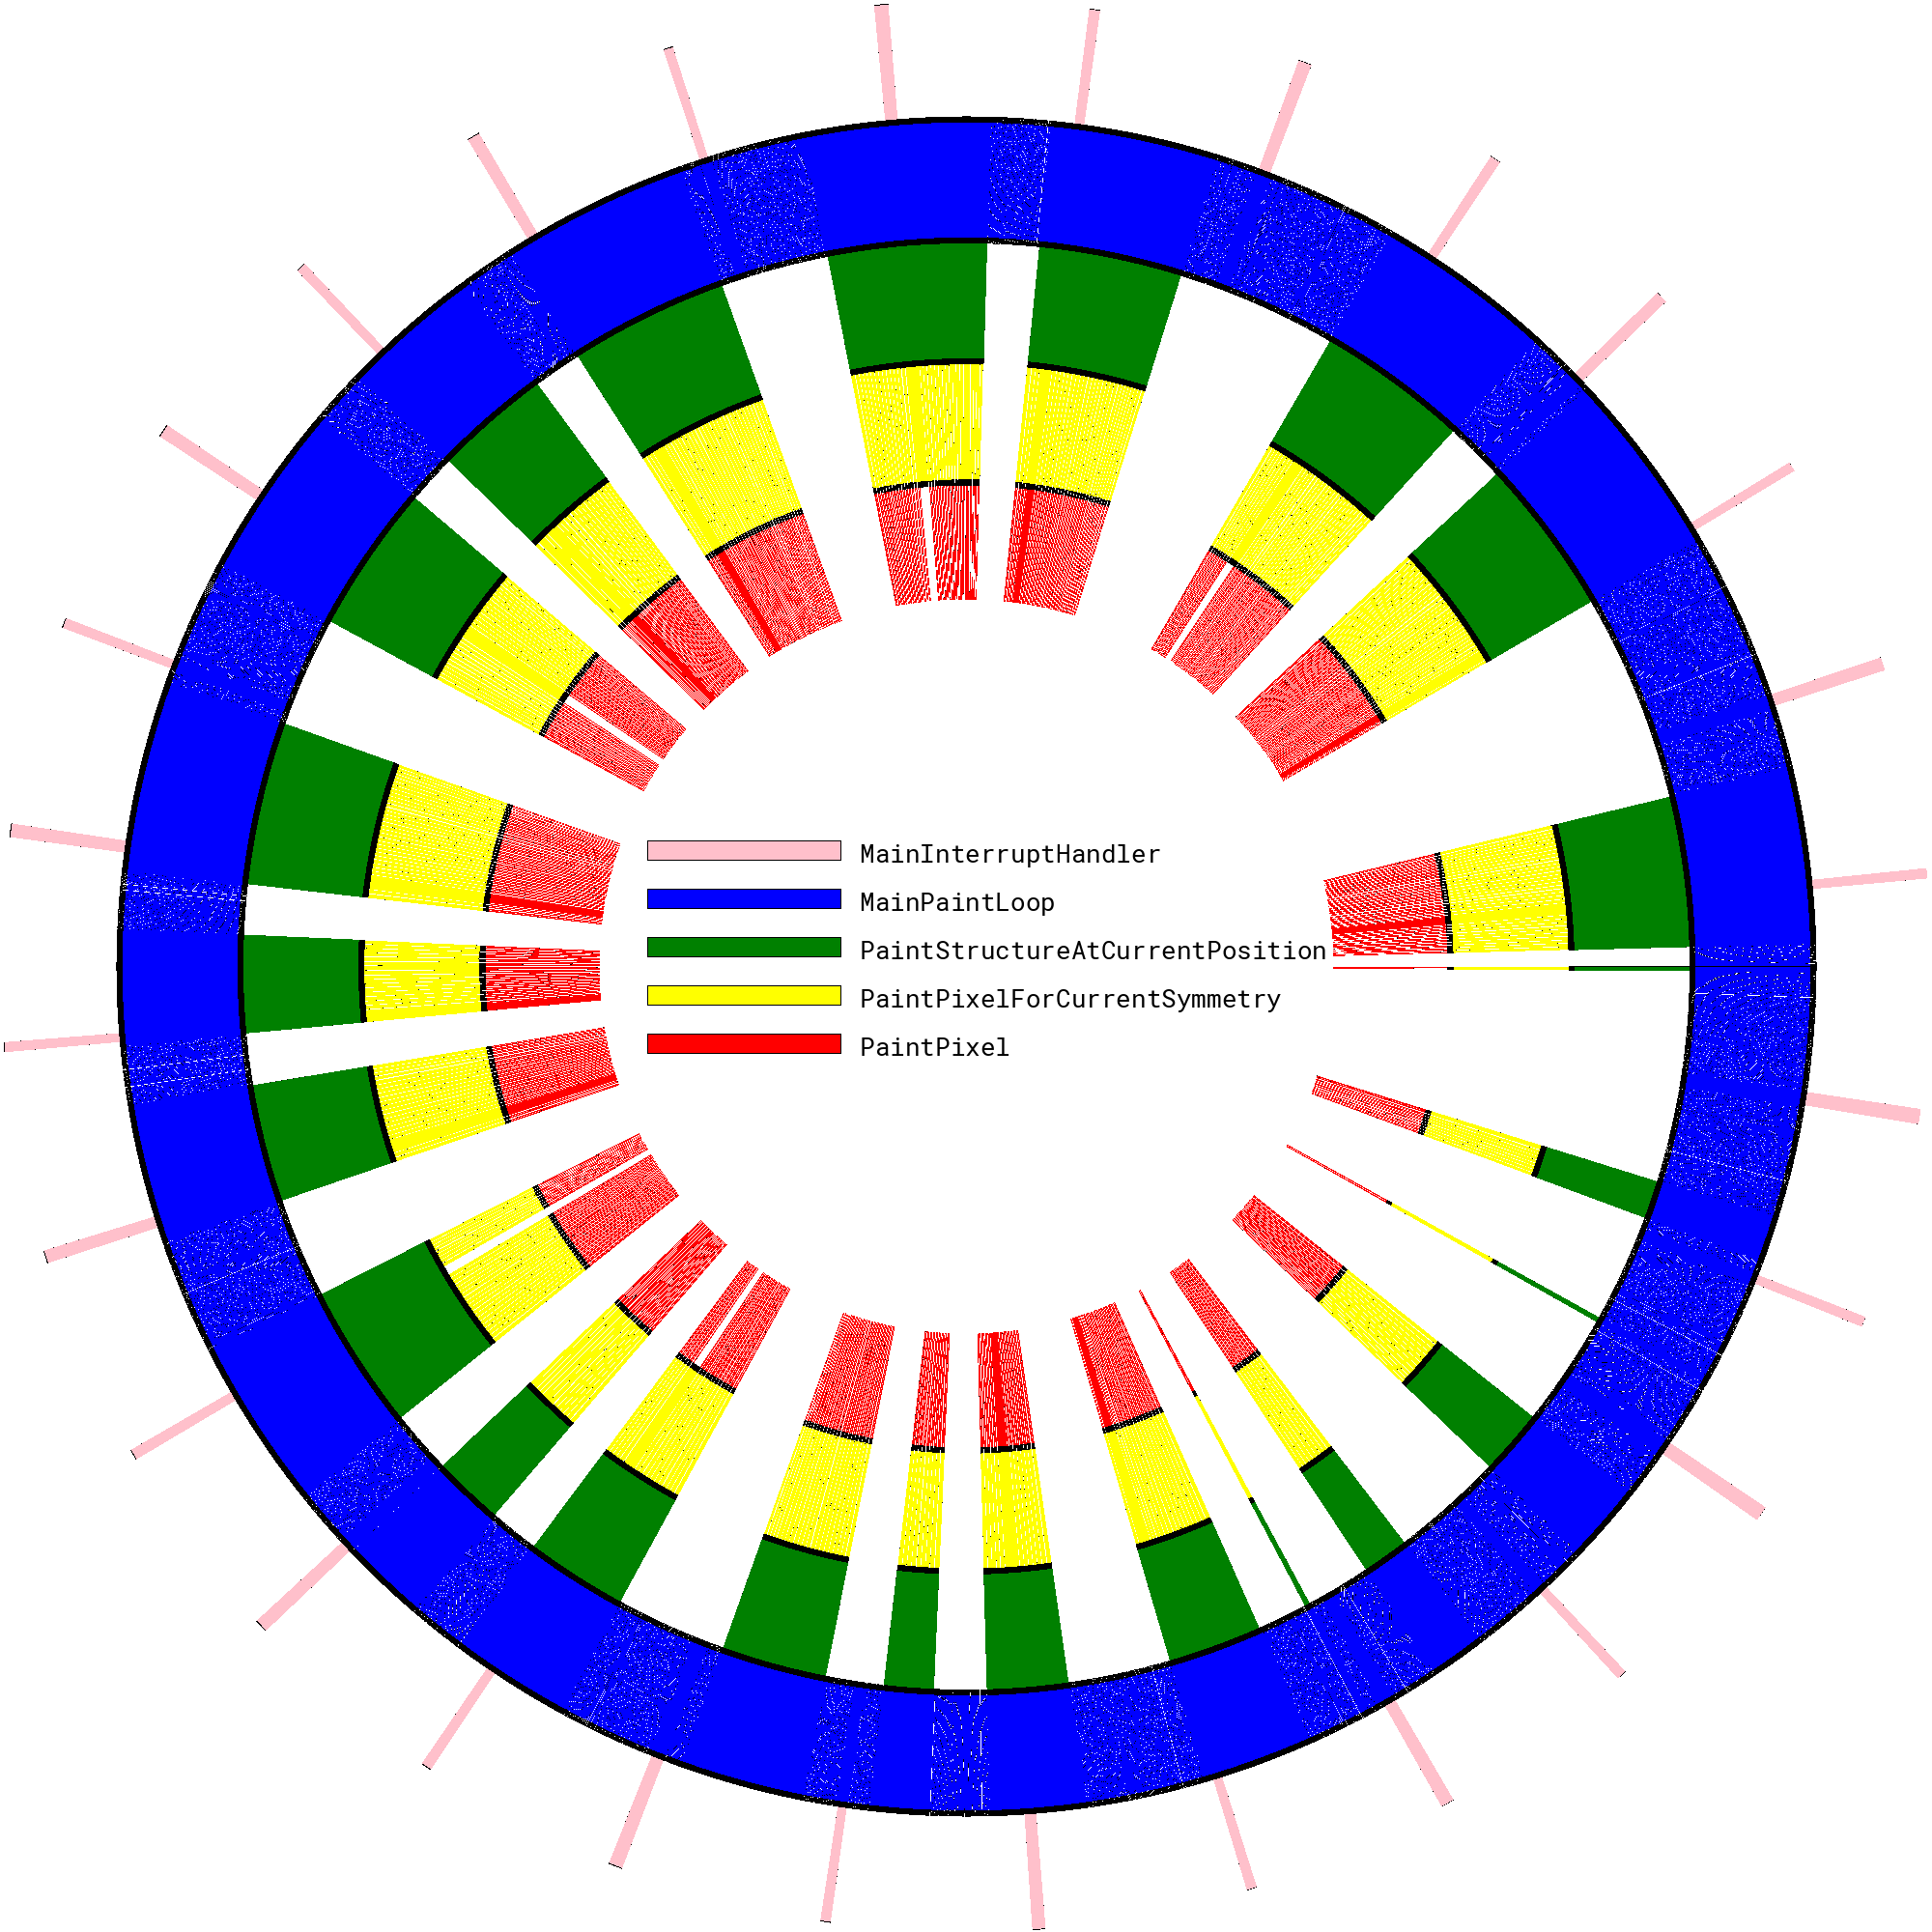
\includegraphics[width=10cm]{src/listing_commentary/execution_cycle.png}%           
  \end{adjustbox}                                                        
\caption{The execution map of a full pattern evolution in the commercial edition of Psychedelia.}                                           
\end{figure}                                                               

\clearpage
\begin{minipage}[b]{0.33\linewidth}
\begin{lrbox}{\mybox}%
\begin{lstlisting}[basicstyle=\ttfamily\tiny,escapechar=\%]
TurnSequenceOff
 LDA #$00
 STA sequencerActive%\index{sequencerActive}%
 STA stepsRemainingInSequencerSequence%\index{stepsRemainingInSequencerSequence}%
 JMP DisplaySequencerState%\index{DisplaySequencerState}%

MaybeVPressed
 CMP #KEY_V
 BNE MaybeOPressed

 LDA #SEQUENCER_SPEED
 STA currentVariableMode%\index{currentVariableMode}%
 RTS

MaybeOPressed
 CMP #KEY_O
 BNE MaybeAsteriskPressed

 LDA #PULSE_WIDTH
 STA currentVariableMode%\index{currentVariableMode}%
 RTS

MaybeAsteriskPressed
 CMP #KEY_ASTERISK
 BNE MaybeRPressed

 LDA #BASE_LEVEL
 STA currentVariableMode%\index{currentVariableMode}%
 RTS

MaybeRPressed
 CMP #KEY_R
 BNE MaybeUpArrowPressed
 JMP StopOrStartRecording%\index{StopOrStartRecording}%

MaybeUpArrowPressed
 CMP #KEY_UP
 BNE MaybeAPressed
 INC pixelShapeIndex%\index{pixelShapeIndex}%
 LDA pixelShapeIndex%\index{pixelShapeIndex}%
 AND #$0F
 TAY
 LDA pixelShapeArray,Y

 LDX #$00
_Loop   STA SCREEN_RAM + $0000,X
 STA SCREEN_RAM + $0100,X
 STA SCREEN_RAM + $0200,X
 STA SCREEN_RAM + $02C0,X
 DEX
 BNE _Loop
 STA currentPixel
 RTS

MaybeAPressed
 CMP #KEY_A
 BNE FinalReturnFromKeyboardCheck

 LDA demoModeActive%\index{demoModeActive}%
 EOR #$01
 STA demoModeActive%\index{demoModeActive}%
 RTS

FinalReturnFromKeyboardCheck
 RTS

initialTimeBetweenKeyStrokes   
 .BYTE $10

;
;   5     5  
;  4       4 
; 5 3 2 2 3 5
;    1   1   
;   2 0 0 2  
;      6     
;   2 0 0 2  
;    1   1   
; 5 3 2 2 3 5
;  4       4 
;   5     5  
multicrossXPosArray%\index{multicrossXPosArray}%
.BYTE $01,$01,$FF,$FF,$55
.BYTE $02,$02,$FE,$FE,$55
.BYTE $01,$03,$03,$01,$FF
.BYTE $FD,$FD,$FF,$55
.BYTE $03,$03,$FD,$FD,$55
.BYTE $04,$04,$FC,$FC,$55
.BYTE $03,$05,$05,$03,$FD
.BYTE $FB,$FB,$FD,$55
.BYTE $00,$55
multicrossYPosArray%\index{multicrossYPosArray}%
.BYTE $FF,$01,$01,$FF,$55
.BYTE $FE,$02,$02,$FE,$55
.BYTE $FD,$FF,$01,$03,$03
.BYTE $01,$FF,$FD,$55
.BYTE $FD,$03,$03,$FD,$55
.BYTE $FC,$04,$04,$FC,$55
.BYTE $FB,$FD,$03,$05,$05
.BYTE $03,$FD,$FB,$55
.BYTE $00,$55


\end{lstlisting}
\end{lrbox}%
\scalebox{0.8}{\usebox{\mybox}}
\end{minipage}
\hspace{-0.1cm}
\begin{minipage}[b]{0.33\linewidth}
\begin{lrbox}{\mybox}%
\begin{lstlisting}[basicstyle=\ttfamily\tiny,escapechar=\%]
;
;       5      
;       4      
;       3      
;       2      
;       1      
;       0      
; 5432106012345
;       0      
;       1      
;       2      
;       3      
;       4      
;       5      

pulsarXPosArray%\index{pulsarXPosArray}%
.BYTE $00,$01,$00,$FF,$55
.BYTE $00,$02,$00,$FE,$55
.BYTE $00,$03,$00,$FD,$55
.BYTE $00,$04,$00,$FC,$55
.BYTE $00,$05,$00,$FB,$55
.BYTE $00,$06,$00,$FA,$55
.BYTE $00,$55

pulsarYPosArray%\index{pulsarYPosArray}% 
.BYTE $FF,$00,$01,$00,$55
.BYTE $FE,$00,$02,$00,$55
.BYTE $FD,$00,$03,$00,$55
.BYTE $FC,$00,$04,$00,$55
.BYTE $FB,$00,$05,$00,$55
.BYTE $FA,$00,$06,$00,$55
.BYTE $00,$55

statusLineBuffer%\index{statusLineBuffer}%                
.BYTE $FF,$FF,$FF,$FF,$FF,$FF

dataFreeDigitOne%\index{dataFreeDigitOne}%  .BYTE $FF

dataFreeDigitTwo  .BYTE $FF

dataFreeDigitThree%\index{dataFreeDigitThree}%              
.BYTE $FF,$FF,$FF,$FF,$FF

customPatternValueBufferPtr     
.BYTE $FF,$FF,$FF

customPatternValueBufferMessage 
.BYTE $FF,$FF,$FF,$FF,$FF,$FF,$FF,$FF
.BYTE $FF,$FF,$FF,$FF,$FF,$FF,$FF,$FF
.BYTE $00,$00,$00,$00,$00,$00,$00,$00


;------------------------------
; ClearLastLineOfScreen%\index{ClearLastLineOfScreen}%
;------------------------------
ClearLastLineOfScreen%\index{ClearLastLineOfScreen}%

 LDX #NUM_COLS
_Loop
 LDA #$20
 STA statusLineBuffer%\index{statusLineBuffer}% - $01,X

 STA SCREEN_RAM + $03BF,X

 DEX
 BNE _Loop
 RTS

;------------------------------
; WriteLastLineBufferToScreen%\index{WriteLastLineBufferToScreen}%
;------------------------------
WriteLastLineBufferToScreen%\index{WriteLastLineBufferToScreen}%
 LDX #NUM_COLS
_Loop
 LDA statusLineBuffer%\index{statusLineBuffer}% - $01,X
 AND #$3F
 STA SCREEN_RAM + $03BF,X

 LDA #$0C
 STA COLOR_RAM + $03BF,X

 DEX
 BNE _Loop
 RTS

txtPresetPatternNames
 .TEXT 'STAR ONE        '
 .TEXT 'THE TWIST       '
 .TEXT 'LA LLAMITA      '
 .TEXT 'STAR TWO        '
 .TEXT 'DELTOIDS        '
 .TEXT 'DIFFUSED        '
 .TEXT 'MULTICROSS      '
 .TEXT 'PULSAR          '

txtSymmetrySettingDescriptions
 .TEXT 'NO SYMMETRY     '
 .TEXT 'Y-AXIS SYMMETRY '
 .TEXT 'X-Y SYMMETRY    '
 .TEXT 'X-AXIS SYMMETRY '
 .TEXT 'QUAD SYMMETRY   '

\end{lstlisting}
\end{lrbox}%
\scalebox{0.8}{\usebox{\mybox}}
\end{minipage}
\hspace{-0.1cm}
\begin{minipage}[b]{0.33\linewidth}
\begin{lrbox}{\mybox}%
\begin{lstlisting}[basicstyle=\ttfamily\tiny,escapechar=\%]
;------------------------------
; PaintLineMode%\index{PaintLineMode}%
;------------------------------
PaintLineMode%\index{PaintLineMode}%
 LDA currentValueInColorIndexArray%\index{currentValueInColorIndexArray}%
 AND #$7F
 STA offsetForYPos%\index{offsetForYPos}%

 LDA #NUM_ROWS + 1
 SEC
 SBC offsetForYPos%\index{offsetForYPos}%
 STA pixelYPosition%\index{pixelYPosition}%

 DEC pixelYPosition%\index{pixelYPosition}%

 LDA #$00
 STA currentValueInColorIndexArray%\index{currentValueInColorIndexArray}%

 LDA #ACTIVE
 STA skipPixel%\index{skipPixel}%

 JSR PaintPixelForCurrentSymmetry%\index{PaintPixelForCurrentSymmetry}%
 INC pixelYPosition%\index{pixelYPosition}%
 LDA #NOT_ACTIVE
 STA skipPixel%\index{skipPixel}%

 LDA lineWidth
 EOR #$07
 STA currentValueInColorIndexArray%\index{currentValueInColorIndexArray}%
LineModeLoop
 JSR PaintPixelForCurrentSymmetry%\index{PaintPixelForCurrentSymmetry}%
 INC pixelYPosition%\index{pixelYPosition}%
 INC currentValueInColorIndexArray%\index{currentValueInColorIndexArray}%
 LDA currentValueInColorIndexArray%\index{currentValueInColorIndexArray}%
 CMP #$08
 BNE ResetLineModeColorValue
 JMP CleanUpAndExitLineModePaint

 INC currentValueInColorIndexArray%\index{currentValueInColorIndexArray}%
ResetLineModeColorValue
 STA currentValueInColorIndexArray%\index{currentValueInColorIndexArray}%
 LDA pixelYPosition%\index{pixelYPosition}%
 CMP #NUM_ROWS + 1
 BNE LineModeLoop

CleanUpAndExitLineModePaint
 LDX currentIndexToPixelBuffers%\index{currentIndexToPixelBuffers}%
 DEC currentColorIndexArray%\index{currentColorIndexArray}%,X
 LDA currentColorIndexArray%\index{currentColorIndexArray}%,X
 CMP #$80
 BEQ ResetIndexAndExitLineModePaint
 JMP MainPaintLoop%\index{MainPaintLoop}%

ResetIndexAndExitLineModePaint
 LDA #$FF
 STA currentColorIndexArray%\index{currentColorIndexArray}%,X
 STX previousIndexToPixelBuffers%\index{previousIndexToPixelBuffers}%
 JMP MainPaintLoop%\index{MainPaintLoop}%

lineModeSettingDescriptions
 .TEXT 'LINE MODE: OFF  '
 .TEXT 'LINE MODE: ON   '
;------------------------------
; DrawColorValueBar%\index{DrawColorValueBar}%
;------------------------------
DrawColorValueBar%\index{DrawColorValueBar}%
 LDA colorBarScreenRamHiPtr%\index{colorBarScreenRamHiPtr}%
 PHA
 CLC
 ADC #$D4
 STA colorBarScreenRamHiPtr%\index{colorBarScreenRamHiPtr}%

 LDY #$00
_Loop   LDA colorBarValues,Y
 STA (colorBarScreenRamLoPtr%\index{colorBarScreenRamLoPtr}%),Y
 INY
 CPY #$10
 BNE _Loop

 PLA
 STA colorBarScreenRamHiPtr%\index{colorBarScreenRamHiPtr}%
 LDA #$00
 STA currentNodeInColorBar%\index{currentNodeInColorBar}%
 STA currentCountInColorBar
 STA offsetToColorBar%\index{offsetToColorBar}%
 LDA maxToDrawOnColorBar%\index{maxToDrawOnColorBar}%
 BEQ ReturnEarlyFromColorBar

ColorBarLoop
 LDA offsetToColorBar%\index{offsetToColorBar}%
 CLC
 ADC currentColorBarOffset%\index{currentColorBarOffset}%
 STA offsetToColorBar%\index{offsetToColorBar}%
 LDX offsetToColorBar%\index{offsetToColorBar}%
 LDY currentNodeInColorBar%\index{currentNodeInColorBar}%
 LDA colorBarCharacterArray,X
 STA (colorBarScreenRamLoPtr%\index{colorBarScreenRamLoPtr}%),Y
 CPX #$08
 BNE GoToNextCell

 LDA #$00
 STA offsetToColorBar%\index{offsetToColorBar}%
 INC currentNodeInColorBar%\index{currentNodeInColorBar}%

\end{lstlisting}
\end{lrbox}%
\scalebox{0.8}{\usebox{\mybox}}
\end{minipage}
\begin{minipage}[b]{0.33\linewidth}
\begin{lrbox}{\mybox}%
\begin{lstlisting}[basicstyle=\ttfamily\tiny,escapechar=\%]

GoToNextCell
 INC currentCountInColorBar
 LDA currentCountInColorBar
 CMP maxToDrawOnColorBar%\index{maxToDrawOnColorBar}%
 BNE ColorBarLoop

ReturnEarlyFromColorBar
 RTS

currentColorBarOffset%\index{currentColorBarOffset}%  .BYTE $FF
currentNodeInColorBar%\index{currentNodeInColorBar}%  .BYTE $FF
maxToDrawOnColorBar%\index{maxToDrawOnColorBar}%    .BYTE $FF
currentCountInColorBar .BYTE $FF
offsetToColorBar%\index{offsetToColorBar}%       .BYTE $FF

colorBarCharacterArray
 .BYTE SPACE,LEFT_BAR_ONE_FIFTH
 .BYTE LEFT_BAR_TWO_FIFTHS
 .BYTE LEFT_BAR_TWO_FIFTHS2
 .BYTE LEFT_BAR_THREE_FIFTHS
 .BYTE RIGHT_BAR_ONE_FIFTHS
 .BYTE RIGHT_BAR_TWO_FIFTHS
 .BYTE RIGHT_BAR_TWO_FIFTHS2
 .BYTE SPACE_MAYBE

ResetSelectedVariableAndReturn%\index{ResetSelectedVariableAndReturn}%
 LDA #NOT_ACTIVE
 STA currentVariableMode%\index{currentVariableMode}%
 RTS

;------------------------------
; CheckKeyboardInputForMode
;------------------------------
CheckKeyboardInputForMode
 AND #$80
 BEQ SlidingScaleActive
 JMP CheckKeyboardWhilePromptActive%\index{CheckKeyboardWhilePromptActive}%

SlidingScaleActive
 LDA timerBetweenKeyStrokes%\index{timerBetweenKeyStrokes}%
 BEQ MaybeDisplayVariableSelection
 DEC timerBetweenKeyStrokes%\index{timerBetweenKeyStrokes}%
 JMP DisplayVariableSelection%\index{DisplayVariableSelection}%

MaybeDisplayVariableSelection
 LDA lastKeyPressed%\index{lastKeyPressed}%
 CMP #NO_KEY_PRESSED
 BNE MaybeUpdateVariable
 JMP DisplayVariableSelection%\index{DisplayVariableSelection}%

MaybeUpdateVariable
 LDA #$04
 STA timerBetweenKeyStrokes%\index{timerBetweenKeyStrokes}%

 LDA currentVariableMode%\index{currentVariableMode}%
 CMP #COLOR_CHANGE
 BEQ UpdateColorChange

 CMP #BUFFER_LENGTH
 BNE UpdateVariableDisplay

UpdateColorChange
 LDX #$00
_Loop   LDA currentColorIndexArray%\index{currentColorIndexArray}%,X
 CMP #$FF
 BNE ResetSelectedVariableAndReturn%\index{ResetSelectedVariableAndReturn}%

 INX
 CPX bufferLength%\index{bufferLength}%
 BNE _Loop

 LDA stepsRemainingInSequencerSequence%\index{stepsRemainingInSequencerSequence}%
 BNE ResetSelectedVariableAndReturn%\index{ResetSelectedVariableAndReturn}%

 LDA playbackOrRecordActive%\index{playbackOrRecordActive}%
 CMP #PLAYING_BACK
 BEQ ResetSelectedVariableAndReturn%\index{ResetSelectedVariableAndReturn}%

 LDA demoModeActive%\index{demoModeActive}%
 BNE ResetSelectedVariableAndReturn%\index{ResetSelectedVariableAndReturn}%

 LDA #GENERIC_ACTIVE
 STA currentModeActive%\index{currentModeActive}%
 LDA #$00
 STA currentStepCount%\index{currentStepCount}%

UpdateVariableDisplay
 LDA #>SCREEN_RAM + $03D0
 STA colorBarScreenRamHiPtr%\index{colorBarScreenRamHiPtr}%
 LDA #<SCREEN_RAM + $03D0
 STA colorBarScreenRamLoPtr%\index{colorBarScreenRamLoPtr}%

 LDX currentVariableMode%\index{currentVariableMode}%
 LDA lastKeyPressed%\index{lastKeyPressed}%
 CMP #KEY_GT
 BNE MaybeLeftArrowPressed

 INC presetValueArray%\index{presetValueArray}%,X
 LDA presetValueArray%\index{presetValueArray}%,X
 CMP maxValueForPresetValueArray,X
 BNE MaybeInColorMode%\index{MaybeInColorMode}%
\end{lstlisting}
\end{lrbox}%
\scalebox{0.8}{\usebox{\mybox}}
\end{minipage}
\hspace{-0.1cm}
\begin{minipage}[b]{0.33\linewidth}
\begin{lrbox}{\mybox}%
\begin{lstlisting}[basicstyle=\ttfamily\tiny,escapechar=\%]
 DEC presetValueArray%\index{presetValueArray}%,X
 JMP MaybeInColorMode%\index{MaybeInColorMode}%

MaybeLeftArrowPressed
 CMP #KEY_TRBR
 BNE MaybeInColorMode%\index{MaybeInColorMode}%

 DEC presetValueArray%\index{presetValueArray}%,X
 LDA presetValueArray%\index{presetValueArray}%,X
 CMP minValueForPresetValueArray,X
 BNE MaybeInColorMode%\index{MaybeInColorMode}%
 INC presetValueArray%\index{presetValueArray}%,X

MaybeInColorMode%\index{MaybeInColorMode}%
 CPX #$05
 BNE MaybeEnterPressed

 LDX indexForColorBarDisplay%\index{indexForColorBarDisplay}%
 LDY currentColorSet%\index{currentColorSet}%
 LDA colorValuesPtr,X
 STA presetColorValuesArray%\index{presetColorValuesArray}%,Y

MaybeEnterPressed
 JSR DisplayVariableSelection%\index{DisplayVariableSelection}%
 JMP CheckIfEnterPressed%\index{CheckIfEnterPressed}%

;------------------------------
; DisplayVariableSelection%\index{DisplayVariableSelection}%
;------------------------------
DisplayVariableSelection%\index{DisplayVariableSelection}%
 LDA #>SCREEN_RAM + $03D0
 STA colorBarScreenRamHiPtr%\index{colorBarScreenRamHiPtr}%
 LDA #<SCREEN_RAM + $03D0
 STA colorBarScreenRamLoPtr%\index{colorBarScreenRamLoPtr}%

 LDX currentVariableMode%\index{currentVariableMode}%
 CPX #COLOR_CHANGE
 BNE VariableModeIsNotColorChange

VariableModeIsColorChange
 LDX currentColorSet%\index{currentColorSet}%
 LDA presetColorValuesArray%\index{presetColorValuesArray}%,X

 LDY #$00
_Loop   
 CMP colorValuesPtr,Y
 BEQ FoundColorMatch
 INY
 CPY #DISPLAY_LINE_LENGTH
 BNE _Loop

FoundColorMatch
 STY indexForColorBarDisplay%\index{indexForColorBarDisplay}%
 LDX currentVariableMode%\index{currentVariableMode}%

VariableModeIsNotColorChange
 LDA increaseOffsetForPresetValueArray,X
 STA currentColorBarOffset%\index{currentColorBarOffset}%

 LDA presetValueArray%\index{presetValueArray}%,X
 STA maxToDrawOnColorBar%\index{maxToDrawOnColorBar}%

 TXA
 PHA

 LDA enterWasPressed%\index{enterWasPressed}%
 BNE UpdateVariableLabel

 LDA #$01
 STA enterWasPressed%\index{enterWasPressed}%
 JSR ClearLastLineOfScreen%\index{ClearLastLineOfScreen}%

UpdateVariableLabel
 PLA
 ASL
 ASL
 ASL
 ASL
 TAY

 LDX #$00
_Loop2  
 LDA txtVariableLabels,Y
 STA statusLineBuffer%\index{statusLineBuffer}%,X
 INY
 INX
 CPX #DISPLAY_LINE_LENGTH
 BNE _Loop2

 LDA currentVariableMode%\index{currentVariableMode}%
 CMP #COLOR_CHANGE
 BNE UpdateBarForOtherMode

UpdateBarForColorMode
 LDA #$30
 CLC
 ADC currentColorSet%\index{currentColorSet}%
 STA dataFreeDigitTwo
UpdateBarForOtherMode
 JSR WriteLastLineBufferToScreen%\index{WriteLastLineBufferToScreen}%
 JMP DrawColorValueBar%\index{DrawColorValueBar}%

\end{lstlisting}
\end{lrbox}%
\scalebox{0.8}{\usebox{\mybox}}
\end{minipage}
\hspace{-0.1cm}
\begin{minipage}[b]{0.33\linewidth}
\begin{lrbox}{\mybox}%
\begin{lstlisting}[basicstyle=\ttfamily\tiny,escapechar=\%]
;------------------------------
; CheckIfEnterPressed%\index{CheckIfEnterPressed}%
;------------------------------
CheckIfEnterPressed%\index{CheckIfEnterPressed}%
 LDA lastKeyPressed%\index{lastKeyPressed}%
 CMP #KEY_RETURN
 BEQ EnterHasBeenPressed
 RTS

EnterHasBeenPressed
 LDA currentVariableMode%\index{currentVariableMode}%
 CMP #COLOR_CHANGE
 BNE ReachedLastColor%\index{ReachedLastColor}%

 INC currentColorSet%\index{currentColorSet}%
 LDA currentColorSet%\index{currentColorSet}%
 CMP #$08
 BEQ ReachedLastColor%\index{ReachedLastColor}%
 RTS

ReachedLastColor%\index{ReachedLastColor}%
 LDA #$00
 STA currentVariableMode%\index{currentVariableMode}%
 STA enterWasPressed%\index{enterWasPressed}%
 RTS


maxValueForPresetValueArray       
.BYTE $00,$40,$08,$40,$10,$10,$08
.BYTE $20,$10,$08
minValueForPresetValueArray       
.BYTE $00,$00,$00,$00,$00
.BYTE $00,$00,$00,$00,$00
increaseOffsetForPresetValueArray 
.BYTE $00,$01,$08
.BYTE $01,$04,$08,$08,$02,$04,$08
currentVariableMode%\index{currentVariableMode}%               
.BYTE $00
currentPulseSpeedCounter%\index{currentPulseSpeedCounter}%          
.BYTE $01

txtVariableLabels
 .TEXT '                '
 .TEXT 'SMOOTHING DELAY:'
 .TEXT 'CURSOR SPEED   :'
 .TEXT 'BUFFER LENGTH  :'
 .TEXT 'PULSE SPEED    :'
 .TEXT 'COLOUR 0 SET   :'
 .TEXT 'WIDTH OF LINE  :'
 .TEXT 'SEQUENCER SPEED:'
 .TEXT 'PULSE WIDTH    :'
 .TEXT 'BASE LEVEL     :'

colorValuesPtr
 .BYTE $00

colorBarValues  
.BYTE BLUE,RED,PURPLE,GREEN
.BYTE CYAN,YELLOW,WHITE,ORANGE
.BYTE BROWN,LTRED,GRAY1,GRAY2
.BYTE LTGREEN,LTBLUE,GRAY3

txtTrackingOnOff
 .TEXT 'TRACKING: OFF   '
 .TEXT 'TRACKING: ON    '

;------------------------------
; DisplayPresetMessage%\index{DisplayPresetMessage}%
;------------------------------
DisplayPresetMessage%\index{DisplayPresetMessage}%
 LDA shiftPressed%\index{shiftPressed}%
 AND #$04
 BEQ SelectNewPreset%\index{SelectNewPreset}%
 JMP MaybeEditCustomPattern%\index{MaybeEditCustomPattern}%

SelectNewPreset%\index{SelectNewPreset}%
 TXA
 PHA
 JSR ClearLastLineOfScreen%\index{ClearLastLineOfScreen}%
 LDX #$00
_Loop   LDA txtPreset,X
 STA statusLineBuffer%\index{statusLineBuffer}%,X
 INX
 CPX #DISPLAY_LINE_LENGTH
 BNE _Loop

 PLA
 PHA
 TAX
 BEQ JumpToUpdateCurrentActivePreset

DataFreeDisplayLoop
 INC dataFreeDigitThree%\index{dataFreeDigitThree}%
 LDA dataFreeDigitThree%\index{dataFreeDigitThree}%
 CMP #COLON
 BNE GoToNextDigit
 LDA #'0'
 STA dataFreeDigitThree%\index{dataFreeDigitThree}%
 INC dataFreeDigitTwo
GoToNextDigit
 DEX
 BNE DataFreeDisplayLoop

\end{lstlisting}
\end{lrbox}%
\scalebox{0.8}{\usebox{\mybox}}
\end{minipage}
\begin{minipage}[b]{0.33\linewidth}
\begin{lrbox}{\mybox}%
\begin{lstlisting}[basicstyle=\ttfamily\tiny,escapechar=\%]
JumpToUpdateCurrentActivePreset
 JMP UpdateCurrentActivePreset%\index{UpdateCurrentActivePreset}%

WriteLastLineBufferAndReturn%\index{WriteLastLineBufferAndReturn}%
 JSR WriteLastLineBufferToScreen%\index{WriteLastLineBufferToScreen}%
 RTS

txtPreset
 .TEXT 'PRESET 00      :'

txtPresetActivatedStored
 .TEXT ' ACTIVATED       '
 .TEXT 'DATA STORED    '

shiftPressed%\index{shiftPressed}%
 .BYTE $00

;------------------------------
; UpdateCurrentActivePreset%\index{UpdateCurrentActivePreset}%
;------------------------------
UpdateCurrentActivePreset%\index{UpdateCurrentActivePreset}%
 LDA shiftPressed%\index{shiftPressed}%
 AND #SHIFT_PRESSED
 ASL
 ASL
 ASL
 ASL
 TAY

DisplayActivatedOrStored
 LDX #$00
_Loop   
 LDA txtPresetActivatedStored,Y
 STA customPatternValueBufferMessage,X

 INY
 INX
 CPX #DISPLAY_LINE_LENGTH
 BNE _Loop

 LDA shiftPressed%\index{shiftPressed}%
 AND #SHIFT_PRESSED
 BNE StoreCurrentValuesAsPreset

 JMP RefreshPresetData%\index{RefreshPresetData}%

StoreCurrentValuesAsPreset
 PLA
 TAX
 JSR GetPresetPointersUsingXRegister%\index{GetPresetPointersUsingXRegister}%

 LDY #$00
 LDX #$00
_Loop   
 LDA presetValueArray%\index{presetValueArray}%,X
 STA (presetSequenceDataLoPtr%\index{presetSequenceDataLoPtr}%),Y

 INY
 INX
 CPX #$15
 BNE _Loop

 LDA currentPatternElement%\index{currentPatternElement}%
 STA (presetSequenceDataLoPtr%\index{presetSequenceDataLoPtr}%),Y

 INY

 LDA currentSymmetrySetting%\index{currentSymmetrySetting}%
 STA (presetSequenceDataLoPtr%\index{presetSequenceDataLoPtr}%),Y

 JMP WriteLastLineBufferAndReturn%\index{WriteLastLineBufferAndReturn}%

;--------------------------------
; RefreshPresetData%\index{RefreshPresetData}%
;--------------------------------
RefreshPresetData%\index{RefreshPresetData}%
 PLA
 TAX
 JSR GetPresetPointersUsingXRegister%\index{GetPresetPointersUsingXRegister}%

 LDY #BUFFER_LENGTH
 LDA (presetSequenceDataLoPtr%\index{presetSequenceDataLoPtr}%),Y
 CMP bufferLength%\index{bufferLength}%
 BEQ MaybeReloadPresetData

 JSR ResetCurrentActiveMode%\index{ResetCurrentActiveMode}%
 JMP LoadSelectedPresetSequence%\index{LoadSelectedPresetSequence}%

MaybeReloadPresetData
 LDX #$00
 LDY #SEQUENCER_SPEED
_Loop   
 LDA (presetSequenceDataLoPtr%\index{presetSequenceDataLoPtr}%),Y
 CMP presetColorValuesArray%\index{presetColorValuesArray}%,X
 BNE LoadSelectedPresetSequence%\index{LoadSelectedPresetSequence}%
 INY
 INX
 CPX #len(presetColorValuesArray%\index{presetColorValuesArray}%)
 BNE _Loop

 JMP LoadSelectedPresetSequence%\index{LoadSelectedPresetSequence}%

;--------------------------------
; LoadSelectedPresetSequence%\index{LoadSelectedPresetSequence}%
;--------------------------------
LoadSelectedPresetSequence%\index{LoadSelectedPresetSequence}%
 LDA #GENERIC_ACTIVE
 STA currentModeActive%\index{currentModeActive}%

\end{lstlisting}
\end{lrbox}%
\scalebox{0.8}{\usebox{\mybox}}
\end{minipage}
\hspace{-0.1cm}
\begin{minipage}[b]{0.33\linewidth}
\begin{lrbox}{\mybox}%
\begin{lstlisting}[basicstyle=\ttfamily\tiny,escapechar=\%]
 LDY #COLOR_BAR_CURRENT
_Loop   
 LDA (presetSequenceDataLoPtr%\index{presetSequenceDataLoPtr}%),Y
 STA presetValueArray%\index{presetValueArray}%,Y
 INY
 CPY #$15
 BNE _Loop

 LDA (presetSequenceDataLoPtr%\index{presetSequenceDataLoPtr}%),Y
 STA currentPatternElement%\index{currentPatternElement}%
 INY
 LDA (presetSequenceDataLoPtr%\index{presetSequenceDataLoPtr}%),Y
 STA currentSymmetrySetting%\index{currentSymmetrySetting}%
 JMP WriteLastLineBufferAndReturn%\index{WriteLastLineBufferAndReturn}%

;------------------------------
; GetPresetPointersUsingXRegister%\index{GetPresetPointersUsingXRegister}%
;------------------------------
GetPresetPointersUsingXRegister%\index{GetPresetPointersUsingXRegister}%
 LDA #>presetSequenceData%\index{presetSequenceData}%
 STA presetSequenceDataHiPtr%\index{presetSequenceDataHiPtr}%
 LDA #<presetSequenceData%\index{presetSequenceData}%
 STA presetSequenceDataLoPtr%\index{presetSequenceDataLoPtr}%
 TXA
 BEQ ReturnFromPresetPointers

_Loop   LDA presetSequenceDataLoPtr%\index{presetSequenceDataLoPtr}%
 CLC
 ADC #$20
 STA presetSequenceDataLoPtr%\index{presetSequenceDataLoPtr}%
 LDA presetSequenceDataHiPtr%\index{presetSequenceDataHiPtr}%
 ADC #$00
 STA presetSequenceDataHiPtr%\index{presetSequenceDataHiPtr}%
 DEX
 BNE _Loop
ReturnFromPresetPointers
 RTS

;------------------------------
; ResetCurrentActiveMode%\index{ResetCurrentActiveMode}%
;------------------------------
ResetCurrentActiveMode%\index{ResetCurrentActiveMode}%
 LDA #GENERIC_ACTIVE
 STA currentModeActive%\index{currentModeActive}%
 LDA #$00
 STA currentStepCount%\index{currentStepCount}%
 RTS

currentModeActive%\index{currentModeActive}%  .BYTE $00
;------------------------------
; ReinitializeScreen%\index{ReinitializeScreen}%
;------------------------------
ReinitializeScreen%\index{ReinitializeScreen}%
 LDA #$00
 STA currentIndexToPixelBuffers%\index{currentIndexToPixelBuffers}%
 STA previousIndexToPixelBuffers%\index{previousIndexToPixelBuffers}%

 LDX #$00
 LDA #$FF
_Loop   STA currentColorIndexArray%\index{currentColorIndexArray}%,X
 INX
 CPX #PIXEL_BUFFER_LENGTH
 BNE _Loop

 LDA #$00
 STA currentModeActive%\index{currentModeActive}%
 JMP InitializeScreenWithInitCharacter%\index{InitializeScreenWithInitCharacter}%

enterWasPressed%\index{enterWasPressed}%  .BYTE $00
functionKeyIndex%\index{functionKeyIndex}% .BYTE $00
;------------------------------
; LoadOrProgramBurstGenerator%\index{LoadOrProgramBurstGenerator}%
;------------------------------
LoadOrProgramBurstGenerator%\index{LoadOrProgramBurstGenerator}%
 JSR ClearLastLineOfScreen%\index{ClearLastLineOfScreen}%
 LDA shiftPressed%\index{shiftPressed}%
 AND #SHIFT_PRESSED
 BEQ PointToBurstData

 LDX #$00
_Loop   LDA txtDataFree,X
 STA statusLineBuffer%\index{statusLineBuffer}%,X
 INX
 CPX #DISPLAY_LINE_LENGTH
 BNE _Loop
 JSR WriteLastLineBufferToScreen%\index{WriteLastLineBufferToScreen}%

PointToBurstData
 LDA #>burstGeneratorF1%\index{burstGeneratorF1}%
 STA currentSequencePtrHi%\index{currentSequencePtrHi}%
 LDX functionKeyIndex%\index{functionKeyIndex}%
 LDA functionKeyToSequenceArray,X
 STA currentSequencePtrLo%\index{currentSequencePtrLo}%

 LDA shiftPressed%\index{shiftPressed}%
 AND #SHIFT_PRESSED
 BEQ LoadBurstDataInstead

 LDA #$10
 STA currentDataFree%\index{currentDataFree}%

 LDY #$00
 LDA currentSymmetrySetting%\index{currentSymmetrySetting}%
 STA (currentSequencePtrLo%\index{currentSequencePtrLo}%),Y
 LDA smoothingDelay%\index{smoothingDelay}%
 INY
 STA (currentSequencePtrLo%\index{currentSequencePtrLo}%),Y
 RTS

\end{lstlisting}
\end{lrbox}%
\scalebox{0.8}{\usebox{\mybox}}
\end{minipage}
\hspace{-0.1cm}
\begin{minipage}[b]{0.33\linewidth}
\begin{lrbox}{\mybox}%
\begin{lstlisting}[basicstyle=\ttfamily\tiny,escapechar=\%]

LoadBurstDataInstead
 LDA #GENERIC_ACTIVE
 STA sequencerActive%\index{sequencerActive}%
 JMP LoadBurstData%\index{LoadBurstData}%

functionKeyToSequenceArray   
.BYTE <burstGeneratorF1%\index{burstGeneratorF1}%,<burstGeneratorF2%\index{burstGeneratorF2}%
.BYTE <burstGeneratorF3%\index{burstGeneratorF3}%,<burstGeneratorF4%\index{burstGeneratorF4}%

txtDataFree
 .TEXT 'DATA: 000 FREE  '

functionKeys
 .BYTE $04,$05,$06,$03

currentDataFree%\index{currentDataFree}%   .BYTE $FF,$60
;------------------------------
; CheckKeyboardWhilePromptActive%\index{CheckKeyboardWhilePromptActive}%
;------------------------------
CheckKeyboardWhilePromptActive%\index{CheckKeyboardWhilePromptActive}%
 LDA currentVariableMode%\index{currentVariableMode}%
 CMP #CUSTOM_PRESET_ACTIVE
 BNE MaybeSavingActive

 JMP CheckInputForCustomPresets

MaybeSavingActive
 CMP #SAVING_ACTIVE
 BNE MaybeLoadingActive
 JMP CheckInputWhileSavePromptActive

MaybeLoadingActive
 CMP #LOADING_ACTIVE
 BNE SequencerOrBurstActive
 JMP CheckInputWhileLoadAbortActive

SequencerOrBurstActive
 LDA #'0'
 STA dataFreeDigitOne%\index{dataFreeDigitOne}%
 STA dataFreeDigitTwo
 STA dataFreeDigitThree%\index{dataFreeDigitThree}%
 LDX currentDataFree%\index{currentDataFree}%
 BNE UpdateDataFreeLoop%\index{UpdateDataFreeLoop}%
 JMP ReturnPressed%\index{ReturnPressed}%

UpdateDataFreeLoop%\index{UpdateDataFreeLoop}%
 INC dataFreeDigitThree%\index{dataFreeDigitThree}%
 LDA dataFreeDigitThree%\index{dataFreeDigitThree}%
 CMP #$3A
 BNE DecrementDataFreeCounterAndLoop%\index{DecrementDataFreeCounterAndLoop}%
 LDA #'0'
 STA dataFreeDigitThree%\index{dataFreeDigitThree}%
 INC dataFreeDigitTwo
 LDA dataFreeDigitTwo
 CMP #$3A
 BNE DecrementDataFreeCounterAndLoop%\index{DecrementDataFreeCounterAndLoop}%
 LDA #'0'
 STA dataFreeDigitTwo
 INC dataFreeDigitOne%\index{dataFreeDigitOne}%
DecrementDataFreeCounterAndLoop%\index{DecrementDataFreeCounterAndLoop}%
 DEX
 BNE UpdateDataFreeLoop%\index{UpdateDataFreeLoop}%

 JSR UpdateDataFreeDisplay%\index{UpdateDataFreeDisplay}%

 LDA customPromptsActive%\index{customPromptsActive}%
 BEQ CheckForInputDuringPrompt

 LDA lastKeyPressed%\index{lastKeyPressed}%
 CMP #NO_KEY_PRESSED
 BEQ ResetPromptAndReturn
 RTS

ResetPromptAndReturn
 LDA #NOT_ACTIVE
 STA customPromptsActive%\index{customPromptsActive}%
ReturnFromPromptRoutine
 RTS

CheckForInputDuringPrompt
 LDA lastKeyPressed%\index{lastKeyPressed}%
 CMP #NO_KEY_PRESSED
 BEQ ReturnFromPromptRoutine

 LDX #ACTIVE
 STX customPromptsActive%\index{customPromptsActive}%

 CMP #KEY_LEFT
 BEQ LeftKeyPressedDuringPrompt

 CMP #KEY_RETURN
 BEQ ReturnPressed%\index{ReturnPressed}%

 CMP #KEY_SPACE
 BNE ReturnFromUpdateDataFree

 JSR UpdateDataFreeDisplay%\index{UpdateDataFreeDisplay}%

 LDA currentDataFree%\index{currentDataFree}%
 STA dataFreeForSequencer%\index{dataFreeForSequencer}%

 LDA currentSequencePtrLo%\index{currentSequencePtrLo}%
 STA prevSequencePtrLo%\index{prevSequencePtrLo}%
 LDA currentSequencePtrHi%\index{currentSequencePtrHi}%
 STA prevSequencePtrHi%\index{prevSequencePtrHi}%

\end{lstlisting}
\end{lrbox}%
\scalebox{0.8}{\usebox{\mybox}}
\end{minipage}
\begin{minipage}[b]{0.33\linewidth}
\begin{lrbox}{\mybox}%
\begin{lstlisting}[basicstyle=\ttfamily\tiny,escapechar=\%]
 LDA #$00
 STA currentVariableMode%\index{currentVariableMode}%
 STA customPromptsActive%\index{customPromptsActive}%
 STA sequencerActive%\index{sequencerActive}%

 LDY #$02
 LDA #$FF
 STA (currentSequencePtrLo%\index{currentSequencePtrLo}%),Y

ReturnFromUpdateDataFree
 RTS

LeftKeyPressedDuringPrompt
 LDY #$02
 LDA shiftKey%\index{shiftKey}%
 AND #$01
 BEQ ShiftAndLeftPressed

 LDA #$C0
 JMP StoreInSequenceData

ShiftAndLeftPressed
 LDA cursorXPosition%\index{cursorXPosition}%

StoreInSequenceData
 STA (currentSequencePtrLo%\index{currentSequencePtrLo}%),Y

 LDA cursorYPosition%\index{cursorYPosition}%
 INY
 STA (currentSequencePtrLo%\index{currentSequencePtrLo}%),Y

 LDA currentPatternElement%\index{currentPatternElement}%
 INY
 STA (currentSequencePtrLo%\index{currentSequencePtrLo}%),Y

 LDA currentSequencePtrLo%\index{currentSequencePtrLo}%
 CLC
 ADC #OFFSET_TO_NEXT_BURST
 STA currentSequencePtrLo%\index{currentSequencePtrLo}%

 LDA currentSequencePtrHi%\index{currentSequencePtrHi}%
 ADC #$00
 STA currentSequencePtrHi%\index{currentSequencePtrHi}%

 DEC currentDataFree%\index{currentDataFree}%
 RTS

;------------------------------
; ReturnPressed%\index{ReturnPressed}%
;------------------------------
ReturnPressed%\index{ReturnPressed}%
 JSR UpdateDataFreeDisplay%\index{UpdateDataFreeDisplay}%

 LDA #$FF
 LDY #$02
 STA (currentSequencePtrLo%\index{currentSequencePtrLo}%),Y

 LDA #NOT_ACTIVE
 STA currentVariableMode%\index{currentVariableMode}%
 STA customPromptsActive%\index{customPromptsActive}%
 STA dataFreeForSequencer%\index{dataFreeForSequencer}%
 STA sequencerActive%\index{sequencerActive}%

 RTS

customPromptsActive%\index{customPromptsActive}%   .BYTE $00
;------------------------------
; UpdateDataFreeDisplay%\index{UpdateDataFreeDisplay}%
;------------------------------
UpdateDataFreeDisplay%\index{UpdateDataFreeDisplay}%
 LDA dataFreeDigitOne%\index{dataFreeDigitOne}%
 STA SCREEN_RAM + $03C6

 LDA dataFreeDigitTwo
 STA SCREEN_RAM + $03C7

 LDA dataFreeDigitThree%\index{dataFreeDigitThree}%
 STA SCREEN_RAM + $03C8
 RTS

;------------------------------
; LoadBurstData%\index{LoadBurstData}%
;------------------------------
LoadBurstData%\index{LoadBurstData}%
 LDA #NOT_ACTIVE
 STA currentVariableMode%\index{currentVariableMode}%
 TAY
 LDA (currentSequencePtrLo%\index{currentSequencePtrLo}%),Y
 STA prevSymmetrySetting%\index{prevSymmetrySetting}%
 INY
 LDA (currentSequencePtrLo%\index{currentSequencePtrLo}%),Y
 STA burstSmoothingDelay%\index{burstSmoothingDelay}%

LoadNextBurstPosition
 LDY #$02
 INC currentStepCount%\index{currentStepCount}%
 LDA currentStepCount%\index{currentStepCount}%
 CMP bufferLength%\index{bufferLength}%
 BNE DontResetStepCountToZero

 LDA #$00
 STA currentStepCount%\index{currentStepCount}%

DontResetStepCountToZero
 LDX currentStepCount%\index{currentStepCount}%
 LDA currentColorIndexArray%\index{currentColorIndexArray}%,X
 CMP #$FF
 BEQ LoadBurstToBuffers

\end{lstlisting}
\end{lrbox}%
\scalebox{0.8}{\usebox{\mybox}}
\end{minipage}
\hspace{-0.1cm}
\begin{minipage}[b]{0.33\linewidth}
\begin{lrbox}{\mybox}%
\begin{lstlisting}[basicstyle=\ttfamily\tiny,escapechar=\%]
 LDA previousIndexToPixelBuffers%\index{previousIndexToPixelBuffers}%
 AND trackingActivated%\index{trackingActivated}%
 BEQ MoveToNextBurstPosition%\index{MoveToNextBurstPosition}%

 STA currentStepCount%\index{currentStepCount}%
 TAX
 LDA currentColorIndexArray%\index{currentColorIndexArray}%,X
 CMP #$FF
 BNE MoveToNextBurstPosition%\index{MoveToNextBurstPosition}%

LoadBurstToBuffers
 LDA baseLevel%\index{baseLevel}%
 STA currentColorIndexArray%\index{currentColorIndexArray}%,X
 LDA (currentSequencePtrLo%\index{currentSequencePtrLo}%),Y
 CMP #$C0
 BEQ MoveToNextBurstPosition%\index{MoveToNextBurstPosition}%

 STA pixelXPositionArray%\index{pixelXPositionArray}%,X
 INY
 LDA (currentSequencePtrLo%\index{currentSequencePtrLo}%),Y
 STA pixelYPositionArray%\index{pixelYPositionArray}%,X
 INY
 LDA (currentSequencePtrLo%\index{currentSequencePtrLo}%),Y
 STA patternIndexArray%\index{patternIndexArray}%,X
 LDA burstSmoothingDelay%\index{burstSmoothingDelay}%
 STA initialSmoothingDelayArray%\index{initialSmoothingDelayArray}%,X
 STA smoothingDelayArray,X%\index{smoothingDelayArray,X}%
 LDA prevSymmetrySetting%\index{prevSymmetrySetting}%
 STA symmetrySettingForStepCount%\index{symmetrySettingForStepCount}%,X

MoveToNextBurstPosition%\index{MoveToNextBurstPosition}%
 LDA currentSequencePtrLo%\index{currentSequencePtrLo}%
 CLC
 ADC #$03
 STA currentSequencePtrLo%\index{currentSequencePtrLo}%
 LDA currentSequencePtrHi%\index{currentSequencePtrHi}%
 ADC #$00
 STA currentSequencePtrHi%\index{currentSequencePtrHi}%
 LDY #$02
 LDA (currentSequencePtrLo%\index{currentSequencePtrLo}%),Y
 CMP #$FF
 BEQ FinishedLoadingBurstData
 JMP LoadNextBurstPosition

FinishedLoadingBurstData
 LDA #$00
 STA sequencerActive%\index{sequencerActive}%
 RTS

burstSmoothingDelay%\index{burstSmoothingDelay}%   .BYTE $00
prevSymmetrySetting%\index{prevSymmetrySetting}% .BYTE $00
sequencerActive%\index{sequencerActive}%     .BYTE $00
;------------------------------
; ActivateSequencer%\index{ActivateSequencer}%
;------------------------------
ActivateSequencer%\index{ActivateSequencer}%
 LDA #>startOfSequencerData
 STA currentSequencePtrHi%\index{currentSequencePtrHi}%
 LDA #<startOfSequencerData
 STA currentSequencePtrLo%\index{currentSequencePtrLo}%
 LDA #GENERIC_ACTIVE
 STA sequencerActive%\index{sequencerActive}%
 LDA shiftPressed%\index{shiftPressed}%
 AND #SHIFT_PRESSED
 BNE ShiftPressedSoProgramSequencer

 LDA sequencerSpeed%\index{sequencerSpeed}%
 STA stepsRemainingInSequencerSequence%\index{stepsRemainingInSequencerSequence}%
 LDA #NOT_ACTIVE
 STA currentVariableMode%\index{currentVariableMode}%
 JSR DisplaySequencerState%\index{DisplaySequencerState}%
 RTS

ShiftPressedSoProgramSequencer
 LDA dataFreeForSequencer%\index{dataFreeForSequencer}%
 BEQ SetUpNewSequencer
 LDA dataFreeForSequencer%\index{dataFreeForSequencer}%
 STA currentDataFree%\index{currentDataFree}%
 LDA prevSequencePtrLo%\index{prevSequencePtrLo}%
 STA currentSequencePtrLo%\index{currentSequencePtrLo}%
 LDA prevSequencePtrHi%\index{prevSequencePtrHi}%
 STA currentSequencePtrHi%\index{currentSequencePtrHi}%
 JMP DisplaySequFree

SetUpNewSequencer
 LDA #$FF
 STA currentDataFree%\index{currentDataFree}%
 LDA currentSymmetrySetting%\index{currentSymmetrySetting}%
 LDY #$00
 STA (currentSequencePtrLo%\index{currentSequencePtrLo}%),Y
 LDA smoothingDelay%\index{smoothingDelay}%
 INY
 STA (currentSequencePtrLo%\index{currentSequencePtrLo}%),Y

DisplaySequFree
 JSR ClearLastLineOfScreen%\index{ClearLastLineOfScreen}%

 LDX #$00
SequencerTextLoop
 LDA txtSequFree,X
 STA statusLineBuffer%\index{statusLineBuffer}%,X
 INX
 CPX #DISPLAY_LINE_LENGTH
 BNE SequencerTextLoop

 JSR WriteLastLineBufferToScreen%\index{WriteLastLineBufferToScreen}%
 RTS
\end{lstlisting}
\end{lrbox}%
\scalebox{0.8}{\usebox{\mybox}}
\end{minipage}
\begin{minipage}[b]{0.33\linewidth}
\begin{lrbox}{\mybox}%
\begin{lstlisting}[basicstyle=\ttfamily\tiny,escapechar=\%]

;------------------------------
; LoadDataForSequencer%\index{LoadDataForSequencer}%
;------------------------------
LoadDataForSequencer%\index{LoadDataForSequencer}%
 INC currentStepCount%\index{currentStepCount}%
 LDA currentStepCount%\index{currentStepCount}%
 CMP bufferLength%\index{bufferLength}%
 BNE CheckPositionInSequencer

 LDA #$00
 STA currentStepCount%\index{currentStepCount}%

CheckPositionInSequencer
 TAX
 LDA currentColorIndexArray%\index{currentColorIndexArray}%,X
 CMP #$FF
 BEQ LoadValuesFromSequencerData

 LDA previousIndexToPixelBuffers%\index{previousIndexToPixelBuffers}%
 AND trackingActivated%\index{trackingActivated}%
 BEQ MoveToNextPositionInSequencer%\index{MoveToNextPositionInSequencer}%
 TAX
 LDA currentColorIndexArray%\index{currentColorIndexArray}%,X
 CMP #$FF
 BNE MoveToNextPositionInSequencer%\index{MoveToNextPositionInSequencer}%

LoadValuesFromSequencerData
 LDY #$02
 LDA (currentSequencePtrLo%\index{currentSequencePtrLo}%),Y
 CMP #BURST_AND_SEQUENCER_END_SENTINEL
 BEQ MoveToNextPositionInSequencer%\index{MoveToNextPositionInSequencer}%

 LDA baseLevel%\index{baseLevel}%
 STA currentColorIndexArray%\index{currentColorIndexArray}%,X

 LDA startOfSequencerData + $01
 STA initialSmoothingDelayArray%\index{initialSmoothingDelayArray}%,X
 STA smoothingDelayArray,X%\index{smoothingDelayArray,X}%

 LDA startOfSequencerData
 STA symmetrySettingForStepCount%\index{symmetrySettingForStepCount}%,X

 LDY #$02
 LDA (currentSequencePtrLo%\index{currentSequencePtrLo}%),Y
 STA pixelXPositionArray%\index{pixelXPositionArray}%,X

 INY

 LDA (currentSequencePtrLo%\index{currentSequencePtrLo}%),Y
 STA pixelYPositionArray%\index{pixelYPositionArray}%,X
 INY

 LDA (currentSequencePtrLo%\index{currentSequencePtrLo}%),Y
 STA patternIndexArray%\index{patternIndexArray}%,X

MoveToNextPositionInSequencer%\index{MoveToNextPositionInSequencer}%
 LDA currentSequencePtrLo%\index{currentSequencePtrLo}%
 CLC
 ADC #OFFSET_TO_NEXT_BURST
 STA currentSequencePtrLo%\index{currentSequencePtrLo}%
 LDA currentSequencePtrHi%\index{currentSequencePtrHi}%
 ADC #$00
 STA currentSequencePtrHi%\index{currentSequencePtrHi}%
 LDY #$02
 LDA (currentSequencePtrLo%\index{currentSequencePtrLo}%),Y
 CMP #$FF
 BEQ ResetSequencerToStart
 RTS

ResetSequencerToStart
 LDA #<startOfSequencerData
 STA currentSequencePtrLo%\index{currentSequencePtrLo}%
 LDA #>startOfSequencerData
 STA currentSequencePtrHi%\index{currentSequencePtrHi}%
 RTS

stepsRemainingInSequencerSequence%\index{stepsRemainingInSequencerSequence}%   
        .BYTE $00

txtSequFree
 .TEXT 'SEQU: 000 FREE  '

;------------------------------
; DisplaySequencerState%\index{DisplaySequencerState}%
;------------------------------
DisplaySequencerState%\index{DisplaySequencerState}%
 LDA sequencerActive%\index{sequencerActive}%
 AND #$01
 ASL
 ASL
 ASL
 ASL
 TAY
 JSR ClearLastLineOfScreen%\index{ClearLastLineOfScreen}%
 LDX #$00
_Loop   LDA txtSequencer,Y
 STA statusLineBuffer%\index{statusLineBuffer}%,X
 INY
 INX
 CPX #DISPLAY_LINE_LENGTH
 BNE _Loop
 JMP WriteLastLineBufferToScreen%\index{WriteLastLineBufferToScreen}%

txtSequencer
      .TEXT 'SEQUENCER OFF   '
      .TEXT 'SEQUENCER ON    '
\end{lstlisting}
\end{lrbox}%
\scalebox{0.8}{\usebox{\mybox}}
\end{minipage}
\begin{minipage}[b]{0.33\linewidth}
\begin{lrbox}{\mybox}%
\begin{lstlisting}[basicstyle=\ttfamily\tiny,escapechar=\%]
dataFreeForSequencer%\index{dataFreeForSequencer}% .BYTE $00
prevSequencePtrLo%\index{prevSequencePtrLo}%    .BYTE $00
prevSequencePtrHi%\index{prevSequencePtrHi}%    .BYTE $00
currentPulseWidth%\index{currentPulseWidth}%    .BYTE $00

;------------------------------
; StopOrStartRecording%\index{StopOrStartRecording}%
;------------------------------
StopOrStartRecording%\index{StopOrStartRecording}%
 LDA #>dynamicStorage%\index{dynamicStorage}%
 STA recordingStorageHiPtr%\index{recordingStorageHiPtr}%

 LDA #<dynamicStorage%\index{dynamicStorage}%
 STA recordingStorageLoPtr%\index{recordingStorageLoPtr}%

 LDA #$01
 STA recordingOffset%\index{recordingOffset}%

 LDA shiftPressed%\index{shiftPressed}%
 AND #SHIFT_PRESSED
 STA shiftPressed%\index{shiftPressed}%

 LDA playbackOrRecordActive%\index{playbackOrRecordActive}%
 ORA shiftPressed%\index{shiftPressed}%
 EOR #$02
 STA playbackOrRecordActive%\index{playbackOrRecordActive}%

 AND #PLAYING_BACK
 BNE UpdateRecordingDisplay

 JMP DisplayStoppedRecording%\index{DisplayStoppedRecording}%

UpdateRecordingDisplay
 LDA playbackOrRecordActive%\index{playbackOrRecordActive}%
 AND #$01
 ASL
 ASL
 ASL
 ASL
 TAY

 JSR ClearLastLineOfScreen%\index{ClearLastLineOfScreen}%

 LDX #$00
_Loop   LDA txtPlayBackRecord,Y
 STA statusLineBuffer%\index{statusLineBuffer}%,X
 INY
 INX
 CPX #DISPLAY_LINE_LENGTH
 BNE _Loop

 JSR WriteLastLineBufferToScreen%\index{WriteLastLineBufferToScreen}%

 LDA playbackOrRecordActive%\index{playbackOrRecordActive}%
 CMP #RECORDING
 BNE ReseetStateAndReturn

;------------------------------
; InitializeDynamicStorage%\index{InitializeDynamicStorage}%
;------------------------------
InitializeDynamicStorage%\index{InitializeDynamicStorage}%
 LDA #<dynamicStorage%\index{dynamicStorage}%
 STA dynamicStorageLoPtr

 LDA #>dynamicStorage%\index{dynamicStorage}%
 STA dynamicStorageHiPtr%\index{dynamicStorageHiPtr}%

 LDY #$00
 TYA

 LDX #$50
DynamicStorageInitLoop%\index{DynamicStorageInitLoop}%
 STA (dynamicStorageLoPtr),Y
 DEY
 BNE DynamicStorageInitLoop%\index{DynamicStorageInitLoop}%

 INC dynamicStorageHiPtr%\index{dynamicStorageHiPtr}%
 DEX
 BNE DynamicStorageInitLoop%\index{DynamicStorageInitLoop}%

 LDA #$FF
 STA dynamicStorage%\index{dynamicStorage}%
 LDA #$01
 STA dynamicStorage%\index{dynamicStorage}% + $01
 LDA cursorXPosition%\index{cursorXPosition}%
 STA previousCursorXPosition%\index{previousCursorXPosition}%
 LDA cursorYPosition%\index{cursorYPosition}%
 STA previousCursorYPosition%\index{previousCursorYPosition}%
 RTS

ReseetStateAndReturn
 LDA #BLACK
 STA currentColorToPaint%\index{currentColorToPaint}%
 JSR PaintCursorAtCurrentPosition%\index{PaintCursorAtCurrentPosition}%
 LDA previousCursorXPosition%\index{previousCursorXPosition}%
 STA cursorXPosition%\index{cursorXPosition}%
 LDA previousCursorYPosition%\index{previousCursorYPosition}%
 STA cursorYPosition%\index{cursorYPosition}%
 LDA #GENERIC_ACTIVE
 STA displaySavePromptActive%\index{displaySavePromptActive}%
 RTS

txtPlayBackRecord
 .TEXT 'PLAYING BACK',$AE,$AE,$AE,$AE'
 .BYTE RECORDING',$AE,$AE,$AE,$AE,$AE,$AE,$AE

\end{lstlisting}
\end{lrbox}%
\scalebox{0.8}{\usebox{\mybox}}
\end{minipage}
\hspace{-0.1cm}
\begin{minipage}[b]{0.33\linewidth}
\begin{lrbox}{\mybox}%
\begin{lstlisting}[basicstyle=\ttfamily\tiny,escapechar=\%]
;------------------------------
; DisplayStoppedRecording%\index{DisplayStoppedRecording}%
;------------------------------
DisplayStoppedRecording%\index{DisplayStoppedRecording}%
 LDA #NOT_ACTIVE
 STA playbackOrRecordActive%\index{playbackOrRecordActive}%
 STA $D020
 STA displaySavePromptActive%\index{displaySavePromptActive}%
 TAY
 JSR ClearLastLineOfScreen%\index{ClearLastLineOfScreen}%
_Loop   LDA txtStopped,Y
 STA statusLineBuffer%\index{statusLineBuffer}%,Y
 INY
 CPY #DISPLAY_LINE_LENGTH
 BNE _Loop
 JMP WriteLastLineBufferToScreen%\index{WriteLastLineBufferToScreen}%

.enc "petscii"
txtStopped
 .TEXT 'STOPPED         '
.enc "none"
playbackOrRecordActive%\index{playbackOrRecordActive}%
 .BYTE $00

;------------------------------
; RecordJoystickMovements%\index{RecordJoystickMovements}%
;------------------------------
RecordJoystickMovements%\index{RecordJoystickMovements}%
 LDA $DC00
 STA lastJoystickInput%\index{lastJoystickInput}%
 LDY #$00
 CMP (recordingStorageLoPtr%\index{recordingStorageLoPtr}%),Y
 BEQ StoreJoystickMovement

MoveStoragePointer
 LDA recordingStorageLoPtr%\index{recordingStorageLoPtr}%
 CLC
 ADC #$02
 STA recordingStorageLoPtr%\index{recordingStorageLoPtr}%
 LDA recordingStorageHiPtr%\index{recordingStorageHiPtr}%
 ADC #$00
 STA recordingStorageHiPtr%\index{recordingStorageHiPtr}%
 CMP #$80
 BNE ResetStoragePointer
 LDA #$00
 STA storageOfSomeKind
 JMP DisplayStoppedRecording%\index{DisplayStoppedRecording}%

ResetStoragePointer
 LDY #$01
 TYA
 STA (recordingStorageLoPtr%\index{recordingStorageLoPtr}%),Y
 LDA $DC00
 DEY
 STA (recordingStorageLoPtr%\index{recordingStorageLoPtr}%),Y
 LDA recordingStorageHiPtr%\index{recordingStorageHiPtr}%
 SEC
 SBC #$30
 CLC
 ROR
 CLC
 ROR
 CLC
 ROR
 CLC
 ROR
 TAX
 LDA colorBarValues,X
 STA $D020
 RTS

StoreJoystickMovement
 INY
 LDA (recordingStorageLoPtr%\index{recordingStorageLoPtr}%),Y
 CLC
 ADC #$01
 STA (recordingStorageLoPtr%\index{recordingStorageLoPtr}%),Y
 CMP #$FF
 BEQ MoveStoragePointer
 RTS


;------------------------------
; GetJoystickInput%\index{GetJoystickInput}%
;------------------------------
GetJoystickInput%\index{GetJoystickInput}%
 LDA playbackOrRecordActive%\index{playbackOrRecordActive}%
 BEQ MaybeInDemoMode
 CMP #RECORDING
 BNE PlayBackInputs
 JMP RecordJoystickMovements%\index{RecordJoystickMovements}%

PlayBackInputs
 JMP PlaybackRecordedJoystickInputs

MaybeInDemoMode
 LDA demoModeActive%\index{demoModeActive}%
 BEQ GetInputFromJoystick

InDemoMode
 JMP MaybePerformRandomMovement

GetInputFromJoystick
 LDA $DC00
 STA lastJoystickInput%\index{lastJoystickInput}%
 RTS

\end{lstlisting}
\end{lrbox}%
\scalebox{0.8}{\usebox{\mybox}}
\end{minipage}
\begin{minipage}[b]{0.33\linewidth}
\begin{lrbox}{\mybox}%
\begin{lstlisting}[basicstyle=\ttfamily\tiny,escapechar=\%]
PlaybackRecordedJoystickInputs
 DEC recordingOffset%\index{recordingOffset}%
 BEQ GetRecordedByte

 LDY #$00
 LDA (recordingStorageLoPtr%\index{recordingStorageLoPtr}%),Y
 STA lastJoystickInput%\index{lastJoystickInput}%
 RTS

GetRecordedByte
 LDA recordingStorageLoPtr%\index{recordingStorageLoPtr}%
 CLC
 ADC #$02
 STA recordingStorageLoPtr%\index{recordingStorageLoPtr}%

 LDA recordingStorageHiPtr%\index{recordingStorageHiPtr}%
 ADC #$00
 STA recordingStorageHiPtr%\index{recordingStorageHiPtr}%
 CMP #$80
 BEQ NoMoreBytes%\index{NoMoreBytes}%
 LDY #$01
 LDA (recordingStorageLoPtr%\index{recordingStorageLoPtr}%),Y
 BEQ NoMoreBytes%\index{NoMoreBytes}%

 STA recordingOffset%\index{recordingOffset}%
 DEY
 LDA (recordingStorageLoPtr%\index{recordingStorageLoPtr}%),Y
 STA lastJoystickInput%\index{lastJoystickInput}%
 RTS

NoMoreBytes%\index{NoMoreBytes}%
 LDA #>dynamicStorage%\index{dynamicStorage}%
 STA recordingStorageHiPtr%\index{recordingStorageHiPtr}%
 LDA #<dynamicStorage%\index{dynamicStorage}%
 STA recordingStorageLoPtr%\index{recordingStorageLoPtr}%
 LDA #$01
 STA recordingOffset%\index{recordingOffset}%
 LDA #BLACK
 STA currentColorToPaint%\index{currentColorToPaint}%
 JSR PaintCursorAtCurrentPosition%\index{PaintCursorAtCurrentPosition}%
 LDA previousCursorXPosition%\index{previousCursorXPosition}%
 STA cursorXPosition%\index{cursorXPosition}%
 LDA previousCursorYPosition%\index{previousCursorYPosition}%
 STA cursorYPosition%\index{cursorYPosition}%
 RTS

recordingOffset%\index{recordingOffset}%         .BYTE $00
previousCursorXPosition%\index{previousCursorXPosition}% .BYTE $0C
previousCursorYPosition%\index{previousCursorYPosition}% .BYTE $0C
customPatternIndex%\index{customPatternIndex}%      .BYTE $00
displaySavePromptActive%\index{displaySavePromptActive}% .BYTE $00
txtDefineAllLevelPixels
 .TEXT 'DEFINE ALL LEVEL  PIXELS'
;------------------------------
; MaybeEditCustomPattern%\index{MaybeEditCustomPattern}%
;------------------------------
MaybeEditCustomPattern%\index{MaybeEditCustomPattern}%
 TXA
 AND #$08
 BEQ EditCustomPattern
 RTS

EditCustomPattern
 LDA #CUSTOM_PRESET_ACTIVE
 STA currentVariableMode%\index{currentVariableMode}%

 LDA #$00
 STA customPatternLoPtr%\index{customPatternLoPtr}%
 STA displaySavePromptActive%\index{displaySavePromptActive}%
 LDA customPatternHiPtrArray,X
 STA customPatternHiPtr
 TXA
 CLC
 ADC #$08
 STA customPatternIndex%\index{customPatternIndex}%
 JSR ClearLastLineOfScreen%\index{ClearLastLineOfScreen}%

 LDX #$00
_Loop   
 LDA txtDefineAllLevelPixels,X
 STA statusLineBuffer%\index{statusLineBuffer}%,X
 INX
 CPX #NUM_ROWS + 1
 BNE _Loop

 JSR WriteLastLineBufferToScreen%\index{WriteLastLineBufferToScreen}%
 LDA #$06
 STA initialBaseLevelForCustomPresets%\index{initialBaseLevelForCustomPresets}%
 LDY #$00
 TYA
 STA (customPatternLoPtr%\index{customPatternLoPtr}%),Y
 INY
 LDA #$55
 STA (customPatternLoPtr%\index{customPatternLoPtr}%),Y
 LDY #$81
 STA (customPatternLoPtr%\index{customPatternLoPtr}%),Y
 DEY
 LDA #$00
 STA (customPatternLoPtr%\index{customPatternLoPtr}%),Y
 LDA #$07
 STA minIndexToColorValues%\index{minIndexToColorValues}%
 LDA #$01
 STA currentIndexToPresetValue%\index{currentIndexToPresetValue}%
 LDA #CUSTOM_PRESET_MODE_ACTIVE
 STA currentModeActive%\index{currentModeActive}%
 RTS
\end{lstlisting}
\end{lrbox}%
\scalebox{0.8}{\usebox{\mybox}}
\end{minipage}
\clearpage
\rhead[]{Loading and Saving}
\textbf{Lines 1643-2300.} This section on the opposite and following two pages deals with the mechanics of 
allowing the player to record and load play sessions, edit custom patterns, and program a new preset. 

In this regard it is largely uninteresting boilerplate. The entire last page for example deals solely with the
details of saving a session to tape storage and loading a previously saved one.

We won't explore this code in any detail in later chapters. 

\clearpage
\begin{minipage}[b]{0.33\linewidth}
\begin{lrbox}{\mybox}%
\begin{lstlisting}[basicstyle=\ttfamily\tiny,escapechar=\%]
;------------------------------
; HandleCustomPreset%\index{HandleCustomPreset}%
;------------------------------
HandleCustomPreset%\index{HandleCustomPreset}%
 LDA #$13
 STA cursorXPosition%\index{cursorXPosition}%
 LDA #$0C
 STA cursorYPosition%\index{cursorYPosition}%
 JSR ReinitializeScreen%\index{ReinitializeScreen}%

_Loop   
 LDA customPatternIndex%\index{customPatternIndex}%
 STA patternIndex%\index{patternIndex}%

 LDA initialBaseLevelForCustomPresets%\index{initialBaseLevelForCustomPresets}%
 STA currentValueInColorIndexArray%\index{currentValueInColorIndexArray}%

 LDA #$00
 STA currentSymmetrySettingForStep%\index{currentSymmetrySettingForStep}%

 LDA #$13
 STA pixelXPosition%\index{pixelXPosition}%

 LDA #$0C
 STA pixelYPosition%\index{pixelYPosition}%

 JSR PaintStructureAtCurrentPosition%\index{PaintStructureAtCurrentPosition}%

 LDA initialBaseLevelForCustomPresets%\index{initialBaseLevelForCustomPresets}%
 BNE _Loop

 JSR ReinitializeScreen%\index{ReinitializeScreen}%

 LDA #NOT_ACTIVE
 STA currentModeActive%\index{currentModeActive}%
 JMP MainPaintLoop%\index{MainPaintLoop}%

;------------------------------
; CheckInputForCustomPresets
;------------------------------
CheckInputForCustomPresets
 LDA customPromptsActive%\index{customPromptsActive}%
 BEQ CheckForKeyPressDuringCustomPrompt
 LDA lastKeyPressed%\index{lastKeyPressed}%
 CMP #NO_KEY_PRESSED
 BEQ ResetCustomPromptsAndReturn
 RTS

ResetCustomPromptsAndReturn
 LDA #$00
 STA customPromptsActive%\index{customPromptsActive}%
ReturnFromOtherPrompts
 RTS

CheckForKeyPressDuringCustomPrompt
 LDA lastKeyPressed%\index{lastKeyPressed}%
 CMP #NO_KEY_PRESSED
 BEQ ReturnFromOtherPrompts

 LDA #GENERIC_ACTIVE
 STA customPromptsActive%\index{customPromptsActive}%

 LDA lastKeyPressed%\index{lastKeyPressed}%
 CMP #KEY_RETURN
 BEQ EnterPressed%\index{EnterPressed}%

 JMP MaybeLeftArrowPressed2

EnterPressed%\index{EnterPressed}%
 INC currentIndexToPresetValue%\index{currentIndexToPresetValue}%
 LDA #$00
 LDY currentIndexToPresetValue%\index{currentIndexToPresetValue}%
 STA (customPatternLoPtr%\index{customPatternLoPtr}%),Y
 PHA
 TYA
 CLC
 ADC #$80
 TAY
 PLA
 STA (customPatternLoPtr%\index{customPatternLoPtr}%),Y
 INY
 LDA #$55
 STA (customPatternLoPtr%\index{customPatternLoPtr}%),Y
 LDY currentIndexToPresetValue%\index{currentIndexToPresetValue}%
 INY
 STA (customPatternLoPtr%\index{customPatternLoPtr}%),Y
 STY currentIndexToPresetValue%\index{currentIndexToPresetValue}%
 LDA #$07
 STA minIndexToColorValues%\index{minIndexToColorValues}%
 DEC initialBaseLevelForCustomPresets%\index{initialBaseLevelForCustomPresets}%
 BEQ ResetVarModeAndReturn

 LDA initialBaseLevelForCustomPresets%\index{initialBaseLevelForCustomPresets}%
 EOR #$07
 CLC
 ADC #$31
 STA SCREEN_RAM + $03D1

 RTS

ResetVarModeAndReturn
 LDA #$00
 STA currentVariableMode%\index{currentVariableMode}%
 JSR ClearLastLineOfScreen%\index{ClearLastLineOfScreen}%
ReturnFromLeftArrow
 RTS

\end{lstlisting}
\end{lrbox}%
\scalebox{0.8}{\usebox{\mybox}}
\end{minipage}
\begin{minipage}[b]{0.33\linewidth}
\begin{lrbox}{\mybox}%
\begin{lstlisting}[basicstyle=\ttfamily\tiny,escapechar=\%]
MaybeLeftArrowPressed2
 CMP #KEY_LEFT
 BNE ReturnFromLeftArrow

 LDY currentIndexToPresetValue%\index{currentIndexToPresetValue}%
 LDA cursorXPosition%\index{cursorXPosition}%
 SEC
 SBC #$13
 STA (customPatternLoPtr%\index{customPatternLoPtr}%),Y
 INY
 LDA #$55
 STA (customPatternLoPtr%\index{customPatternLoPtr}%),Y
 STY currentIndexToPresetValue%\index{currentIndexToPresetValue}%
 TYA
 CLC
 ADC #$7F
 TAY
 LDA cursorYPosition%\index{cursorYPosition}%
 SEC
 SBC #$0C
 STA (customPatternLoPtr%\index{customPatternLoPtr}%),Y
 INY
 LDA #$55
 STA (customPatternLoPtr%\index{customPatternLoPtr}%),Y
 DEC minIndexToColorValues%\index{minIndexToColorValues}%
 BEQ PressEnter
 RTS

PressEnter
 JMP EnterPressed%\index{EnterPressed}%

;------------------------------
; GetCustomPatternElement%\index{GetCustomPatternElement}%
;------------------------------
GetCustomPatternElement%\index{GetCustomPatternElement}%
 JSR ClearLastLineOfScreen%\index{ClearLastLineOfScreen}%

 LDX #$00
txtPatternLoop
 LDA txtCustomPatterns,X
 STA statusLineBuffer%\index{statusLineBuffer}%,X
 INX
 CPX #$0E
 BNE txtPatternLoop

 LDA currentPatternElement%\index{currentPatternElement}%
 AND #$07
 CLC
 ADC #$30
 STA customPatternValueBufferPtr
 JMP WriteLastLineBufferToScreen%\index{WriteLastLineBufferToScreen}%

.enc "petscii"
txtCustomPatterns .TEXT 'USER SHAPE _0'
.enc "none"
pixelShapeIndex%\index{pixelShapeIndex}% .BYTE $00
pixelShapeArray
 .BYTE BLOCK,CIRCLE,HEART,DIAMOND
 .BYTE CROSS,TOP_RIGHT_TRIANGLE,DONUT
 .BYTE CHECKER,ANDREWS_CROSS,LEFT_HALF
 .BYTE TOP_LEFT_BRACKET,FULL_CHECKER
 .BYTE BOTTOM_RIGHT_SQUARE
 .BYTE BOTTOM_RIGHT_SQUARE2,SPACE_MAYBE,ASTERISK
 .BYTE $47,$4F,$41,$54,$53,$53,$48,$45
 .BYTE $45,$50

;------------------------------
; DisplaySavePromptScreen%\index{DisplaySavePromptScreen}%
;------------------------------
DisplaySavePromptScreen%\index{DisplaySavePromptScreen}%
 LDA #$13
 JSR PRINT
 LDA #GENERIC_ACTIVE
 STA displaySavePromptActive%\index{displaySavePromptActive}%
 JSR InitializeScreenWithInitCharacter%\index{InitializeScreenWithInitCharacter}%

_Loop   LDA tapeSavingInProgress
 BEQ _Loop

MaybeSaveParameters
 CMP #SAVE_PARAMETERS
 BNE MaybeSaveMotions

SaveParameters
 LDA #$01
 LDX #$01
 LDY #$01
 JSR ROM_SETLFS

 LDA #$05
 LDX #$59
 LDY #$1D
 JSR ROM_SETNAM

 LDA #$01
 STA CURRENT_CHAR_COLOR
 LDA #>presetSequenceData%\index{presetSequenceData}%
 STA presetHiPtr%\index{presetHiPtr}%
 LDA #<presetSequenceData%\index{presetSequenceData}%
 STA presetLoPtr%\index{presetLoPtr}%

 LDX #$FF
 LDY #$CF
 LDA #$FE
 JSR ROM_SAVE
 JMP ResetSavingStateAndReturn%\index{ResetSavingStateAndReturn}%

\end{lstlisting}
\end{lrbox}%
\scalebox{0.8}{\usebox{\mybox}}
\end{minipage}
\hspace{-0.1cm}
\begin{minipage}[b]{0.33\linewidth}
\begin{lrbox}{\mybox}%
\begin{lstlisting}[basicstyle=\ttfamily\tiny,escapechar=\%]
MaybeSaveMotions
 CMP #SAVE_MOTIONS
 BNE ContinueSave

SaveMotions
 LDA #$01
 LDX #$01
 LDY #$01
 JSR ROM_SETLFS

 LDA #$05
 LDX #$5E
 LDY #$1D
 JSR ROM_SETNAM

 LDA #WHITE
 STA CURRENT_CHAR_COLOR

 LDA #$30
 STA presetHiPtr%\index{presetHiPtr}%
 STA presetTempHiPtr%\index{presetTempHiPtr}%

 LDA #$00
 STA presetLoPtr%\index{presetLoPtr}%
 STA presetTempLoPtr%\index{presetTempLoPtr}%

 LDY #$00
_Loop2  LDA (presetTempLoPtr%\index{presetTempLoPtr}%),Y
 BEQ ExitSaveLoop
 INC presetTempLoPtr%\index{presetTempLoPtr}%
 BNE _Loop2
 INC presetTempHiPtr%\index{presetTempHiPtr}%
 JMP _Loop2

ExitSaveLoop
 LDX presetTempLoPtr%\index{presetTempLoPtr}%
 LDY presetTempHiPtr%\index{presetTempHiPtr}%

 LDA #$FE
 JSR ROM_SAVE
 JMP ResetSavingStateAndReturn%\index{ResetSavingStateAndReturn}%

ContinueSave
 LDA #$01
 LDX #$01
 LDY #$01
 JSR ROM_SETLFS

 LDA #$00
 JSR ROM_SETNAM

 LDA #WHITE
 STA CURRENT_CHAR_COLOR
 LDA #$00
 JSR ROM_LOAD

 JSR ROM_READST

 AND #$10
 BEQ ResetSavingStateAndReturn%\index{ResetSavingStateAndReturn}%

 JSR DisplayLoadOrAbort%\index{DisplayLoadOrAbort}%

ResetSavingStateAndReturn%\index{ResetSavingStateAndReturn}%
 LDA #NOT_ACTIVE
 STA currentModeActive%\index{currentModeActive}%
 STA displaySavePromptActive%\index{displaySavePromptActive}%
 STA tapeSavingInProgress

 JSR ROM_CLALL

 JSR ReinitializeScreen%\index{ReinitializeScreen}%

 JMP MainPaintLoop%\index{MainPaintLoop}%

 RTS

;------------------------------
; PromptToSave%\index{PromptToSave}%
;------------------------------
PromptToSave%\index{PromptToSave}%
 LDA stepsRemainingInSequencerSequence%\index{stepsRemainingInSequencerSequence}%
 BNE ReturnFromPromptToSave%\index{ReturnFromPromptToSave}%

 LDA playbackOrRecordActive%\index{playbackOrRecordActive}%
 CMP #PLAYING_BACK
 BEQ ReturnFromPromptToSave%\index{ReturnFromPromptToSave}%

 LDA #SAVING_ACTIVE
 STA currentVariableMode%\index{currentVariableMode}%

 LDX #$00
_Loop   LDA txtSavePrompt,X
 STA statusLineBuffer%\index{statusLineBuffer}%,X
 INX
 CPX #NUM_COLS
 BNE _Loop

 LDA #NOT_ACTIVE
 STA tapeSavingInProgress

 JSR WriteLastLineBufferToScreen%\index{WriteLastLineBufferToScreen}%
ReturnFromPromptToSave%\index{ReturnFromPromptToSave}%
 RTS

txtSavePrompt
.TEXT " SAVE (P)ARAMETERS, (M)OTION, (A)BORT?  "

\end{lstlisting}
\end{lrbox}%
\scalebox{0.8}{\usebox{\mybox}}
\end{minipage}
\begin{minipage}[b]{0.33\linewidth}
\begin{lrbox}{\mybox}%
\begin{lstlisting}[basicstyle=\ttfamily\tiny,escapechar=\%]
;------------------------------
; CheckInputWhileSavePromptActive
;------------------------------
CheckInputWhileSavePromptActive
 LDA currentVariableMode%\index{currentVariableMode}%
 CMP #SAVING_ACTIVE
 BEQ MaybeAbort
 RTS

MaybeAbort
 LDA lastKeyPressed%\index{lastKeyPressed}%
 CMP #KEY_A
 BNE MaybeM_Pressed

 LDA #NOT_ACTIVE
 STA currentModeActive%\index{currentModeActive}%

ResetStateAndClearPrompt%\index{ResetStateAndClearPrompt}%
 LDA #NOT_ACTIVE
 STA currentVariableMode%\index{currentVariableMode}%

 JMP ClearLastLineOfScreen%\index{ClearLastLineOfScreen}%

MaybeM_Pressed
 CMP #KEY_M
 BNE MaybeP_Pressed

 LDA #SAVE_MOTIONS
 STA tapeSavingInProgress

 LDA #SAVE_PROMPT_MODE_ACTIVE
 STA currentModeActive%\index{currentModeActive}%

 JMP ResetStateAndClearPrompt%\index{ResetStateAndClearPrompt}%

MaybeP_Pressed
 CMP #KEY_P
 BNE ReturnFromSave%\index{ReturnFromSave}%

 LDA #SAVE_PARAMETERS
 STA tapeSavingInProgress

 LDA #SAVE_PROMPT_MODE_ACTIVE
 STA currentModeActive%\index{currentModeActive}%

 JMP ResetStateAndClearPrompt%\index{ResetStateAndClearPrompt}%

ReturnFromSave%\index{ReturnFromSave}%
 RTS

tapeSavingInProgress   .BYTE $00
;------------------------------
; DisplayLoadOrAbort%\index{DisplayLoadOrAbort}%
;------------------------------
DisplayLoadOrAbort%\index{DisplayLoadOrAbort}%
 LDA stepsRemainingInSequencerSequence%\index{stepsRemainingInSequencerSequence}%
 BNE ReturnFromSave%\index{ReturnFromSave}%

 LDA playbackOrRecordActive%\index{playbackOrRecordActive}%
 CMP #PLAYING_BACK
 BEQ ReturnFromSave%\index{ReturnFromSave}%

 LDA #LOADING_ACTIVE
 STA currentVariableMode%\index{currentVariableMode}%

 LDX #$00
DisplayLoadAbortLoop
 LDA txtContinueLoadOrAbort,X
 STA statusLineBuffer%\index{statusLineBuffer}%,X
 INX
 CPX #NUM_COLS
 BNE DisplayLoadAbortLoop

 LDA #NOT_ACTIVE
 STA tapeSavingInProgress
 JMP WriteLastLineBufferToScreen%\index{WriteLastLineBufferToScreen}%

;------------------------------
; CheckInputWhileLoadAbortActive
;------------------------------
CheckInputWhileLoadAbortActive
 LDA lastKeyPressed%\index{lastKeyPressed}%
 CMP #KEY_A
 BNE MaybeCPressedWhileLoadAbortActitve
 LDA #NOT_ACTIVE
 STA currentVariableMode%\index{currentVariableMode}%
 STA tapeSavingInProgress
 STA currentModeActive%\index{currentModeActive}%
 JMP ClearLastLineOfScreen%\index{ClearLastLineOfScreen}%

MaybeCPressedWhileLoadAbortActitve
 CMP #KEY_C
 BNE ReturnFromInputWhileLoadAbortActive

 LDA #CONTINUE_SAVE
 STA tapeSavingInProgress
 LDA #NOT_ACTIVE
 STA currentVariableMode%\index{currentVariableMode}%
 LDA #SAVE_PROMPT_MODE_ACTIVE
 STA currentModeActive%\index{currentModeActive}%
 JMP ClearLastLineOfScreen%\index{ClearLastLineOfScreen}%

ReturnFromInputWhileLoadAbortActive
 RTS
\end{lstlisting}
\end{lrbox}%
\scalebox{0.8}{\usebox{\mybox}}
\end{minipage}
\begin{minipage}[b]{0.33\linewidth}
\begin{lrbox}{\mybox}%
\begin{lstlisting}[basicstyle=\ttfamily\tiny,escapechar=\%]
txtContinueLoadOrAbort
.TEXT '{C}ONTINUE LOAD@ OR {A}BORT?            '
demoModeActive%\index{demoModeActive}%          .BYTE $00
joystickInputDebounce%\index{joystickInputDebounce}%   .BYTE $01
joystickInputRandomizer%\index{joystickInputRandomizer}% .BYTE $10

;------------------------------
; MaybePerformRandomMovement
;------------------------------
MaybePerformRandomMovement
 DEC joystickInputDebounce%\index{joystickInputDebounce}%
 BEQ PerformRandomJoystickMovement
 RTS

PerformRandomJoystickMovement
 JSR PutRandomByteInAccumulator%\index{PutRandomByteInAccumulator}%
 AND #$1F
 ORA #$01
 STA joystickInputDebounce%\index{joystickInputDebounce}%

 LDA joystickInputRandomizer%\index{joystickInputRandomizer}%
 EOR #$10
 STA joystickInputRandomizer%\index{joystickInputRandomizer}%

 JSR PutRandomByteInAccumulator%\index{PutRandomByteInAccumulator}%
 AND #$0F
 ORA joystickInputRandomizer%\index{joystickInputRandomizer}%
 EOR #$1F
 STA lastJoystickInput%\index{lastJoystickInput}%
 DEC demoModeCountDownToChangePreset

 BEQ SelectRandomPreset
 RTS

SelectRandomPreset
 JSR PutRandomByteInAccumulator%\index{PutRandomByteInAccumulator}%
 AND #$07
 ADC #$20
 STA demoModeCountDownToChangePreset

 JSR PutRandomByteInAccumulator%\index{PutRandomByteInAccumulator}%
 AND #$0F
 TAX

 LDA #$00
 STA shiftPressed%\index{shiftPressed}%
 JMP SelectNewPreset%\index{SelectNewPreset}%

;------------------------------
; MaybeDisplayDemoModeMessage%\index{MaybeDisplayDemoModeMessage}%
;------------------------------
MaybeDisplayDemoModeMessage%\index{MaybeDisplayDemoModeMessage}%
 LDA demoModeActive%\index{demoModeActive}%
 BNE DisplayDemoModeMessage

 JMP ClearLastLineOfScreen%\index{ClearLastLineOfScreen}%

DisplayDemoModeMessage
 LDX #$00

DisplayDemoMsgLoop
 LDA demoMessage,X
 STA statusLineBuffer%\index{statusLineBuffer}%,X
 INX
 CPX #NUM_COLS
 BNE DisplayDemoMsgLoop
 JMP WriteLastLineBufferToScreen%\index{WriteLastLineBufferToScreen}%

demoMessage
 .TEXT "PSYCHEDELIA BY JEFF MINTER"

* = $1FA9
demoModeCountDownToChangePreset .BYTE $20

;------------------------------
; NMIInterruptHandler
;------------------------------
NMIInterruptHandler
 LDX #<CalledFromNMI
 TXS
 LDA #>CalledFromNMI
 PHA
 LDA #$30
 PHA
 LDA #$23
 PHA
 RTI

;------------------------------
; MovePresetDataIntoPosition%\index{MovePresetDataIntoPosition}%
;------------------------------
MovePresetDataIntoPosition%\index{MovePresetDataIntoPosition}%
 LDY #$00
 TYA
 STA copyFromLoPtr
 STA copyToLoPtr
 LDA #>presetSequenceDataSource
 STA copyFromHiPtr
 LDA #>presetSequenceData%\index{presetSequenceData}%
 STA copyToHiPtr

 LDX #$10
_Loop   LDA (copyFromLoPtr),Y
 STA (copyToLoPtr),Y
 DEY
 BNE _Loop
\end{lstlisting}
\end{lrbox}%
\scalebox{0.8}{\usebox{\mybox}}
\end{minipage}
\begin{minipage}[b]{0.33\linewidth}
\begin{lrbox}{\mybox}%
\begin{lstlisting}[basicstyle=\ttfamily\tiny,escapechar=\%]

 INC copyFromHiPtr
 INC copyToHiPtr
 DEX
 BNE _Loop

 LDX #$09
_Loop2  LDA originalStorageOfSomeKind,X
 STA storageOfSomeKind,X
 DEX
 BNE _Loop2
 RTS

originalStorageOfSomeKind=*-$01
 .BYTE $30,$0C,$30,$0C,$C3,$C2,$CD,$38
 .BYTE $30,$00,$00,$00,$00,$00,$00,$00
 .BYTE $00,$00,$00,$00,$00,$00,$00,$00
 .BYTE $00,$00,$00,$00,$00,$00

\end{lstlisting}
\end{lrbox}%
\scalebox{0.8}{\usebox{\mybox}}
\end{minipage}
\begin{minipage}[b]{0.33\linewidth}
\begin{lrbox}{\mybox}%
\begin{lstlisting}[basicstyle=\ttfamily\tiny,escapechar=\%]
preset1
.BYTE $00 ; unusedPresetByte
.BYTE $0C ; smoothingDelay%\index{smoothingDelay}%
.BYTE $02 ; cursorSpeed
.BYTE $28 ; bufferLength%\index{bufferLength}%
.BYTE $01 ; pulseSpeed
.BYTE $0E ; indexForColorBarDisplay%\index{indexForColorBarDisplay}%
.BYTE $07 ; lineWidth
.BYTE $08 ; sequencerSpeed%\index{sequencerSpeed}%
.BYTE $01 ; pulseWidth
.BYTE $07 ; baseLevel%\index{baseLevel}%
; presetColorValuesArray%\index{presetColorValuesArray}%: 
.BYTE BLACK,BROWN,RED,ORANGE,PURPLE,LTRED,BLUE,LTBLUE
.BYTE $FF ; trackingActivated%\index{trackingActivated}%
.BYTE $00 ; lineModeActivated%\index{lineModeActivated}%
.BYTE $01 ; presetIndex
.BYTE $01 ; currentPatternElement%\index{currentPatternElement}%
.BYTE $04 ; currentSymmetrySetting%\index{currentSymmetrySetting}%

preset2
.BYTE $00 ; unusedPresetByte
.BYTE $0B ; smoothingDelay%\index{smoothingDelay}%
.BYTE $02 ; cursorSpeed
.BYTE $28 ; bufferLength%\index{bufferLength}%
.BYTE $01 ; pulseSpeed
.BYTE $01 ; indexForColorBarDisplay%\index{indexForColorBarDisplay}%
.BYTE $07 ; lineWidth
.BYTE $0B ; sequencerSpeed%\index{sequencerSpeed}%
.BYTE $01 ; pulseWidth
.BYTE $07 ; baseLevel%\index{baseLevel}%
; presetColorValuesArray%\index{presetColorValuesArray}%: 
.BYTE BLACK,BLUE,LTBLUE,CYAN,LTGREEN,GREEN,LTBLUE,BLUE
.BYTE $FF ; trackingActivated%\index{trackingActivated}%
.BYTE $00 ; lineModeActivated%\index{lineModeActivated}%
.BYTE $05 ; presetIndex
.BYTE $05 ; currentPatternElement%\index{currentPatternElement}%
.BYTE $01 ; currentSymmetrySetting%\index{currentSymmetrySetting}%

preset3
.BYTE $00 ; unusedPresetByte
.BYTE $04 ; smoothingDelay%\index{smoothingDelay}%
.BYTE $02 ; cursorSpeed
.BYTE $26 ; bufferLength%\index{bufferLength}%
.BYTE $01 ; pulseSpeed
.BYTE $01 ; indexForColorBarDisplay%\index{indexForColorBarDisplay}%
.BYTE $07 ; lineWidth
.BYTE $0A ; sequencerSpeed%\index{sequencerSpeed}%
.BYTE $01 ; pulseWidth
.BYTE $07 ; baseLevel%\index{baseLevel}%
; presetColorValuesArray%\index{presetColorValuesArray}%: 
.BYTE BLACK,RED,PURPLE,LTRED,LTGREEN,CYAN,LTBLUE,BLUE
.BYTE $00 ; trackingActivated%\index{trackingActivated}%
.BYTE $00 ; lineModeActivated%\index{lineModeActivated}%
.BYTE $0E ; presetIndex
.BYTE $0E ; currentPatternElement%\index{currentPatternElement}%
.BYTE $02 ; currentSymmetrySetting%\index{currentSymmetrySetting}%

preset4
.BYTE $00 ; unusedPresetByte
.BYTE $0C ; smoothingDelay%\index{smoothingDelay}%
.BYTE $01 ; cursorSpeed
.BYTE $2B ; bufferLength%\index{bufferLength}%
.BYTE $01 ; pulseSpeed
.BYTE $07 ; indexForColorBarDisplay%\index{indexForColorBarDisplay}%
.BYTE $07 ; lineWidth
.BYTE $08 ; sequencerSpeed%\index{sequencerSpeed}%
.BYTE $01 ; pulseWidth
.BYTE $07 ; baseLevel%\index{baseLevel}%
; presetColorValuesArray%\index{presetColorValuesArray}%: 
.BYTE BLACK,GRAY1,BLUE,GRAY2,PURPLE,GRAY3,CYAN,WHITE
.BYTE $00 ; trackingActivated%\index{trackingActivated}%
.BYTE $00 ; lineModeActivated%\index{lineModeActivated}%
.BYTE $01 ; presetIndex
.BYTE $01 ; currentPatternElement%\index{currentPatternElement}%
.BYTE $01 ; currentSymmetrySetting%\index{currentSymmetrySetting}%

preset5
.BYTE $00 ; unusedPresetByte
.BYTE $0C ; smoothingDelay%\index{smoothingDelay}%
.BYTE $02 ; cursorSpeed
.BYTE $2B ; bufferLength%\index{bufferLength}%
.BYTE $01 ; pulseSpeed
.BYTE $07 ; indexForColorBarDisplay%\index{indexForColorBarDisplay}%
.BYTE $07 ; lineWidth
.BYTE $0C ; sequencerSpeed%\index{sequencerSpeed}%
.BYTE $01 ; pulseWidth
.BYTE $07 ; baseLevel%\index{baseLevel}%
; presetColorValuesArray%\index{presetColorValuesArray}%: 
.BYTE BLACK,GRAY1,BLUE,GRAY2,PURPLE,GRAY3,CYAN,WHITE
.BYTE $00 ; trackingActivated%\index{trackingActivated}%
.BYTE $00 ; lineModeActivated%\index{lineModeActivated}%
.BYTE $06 ; presetIndex
.BYTE $06 ; currentPatternElement%\index{currentPatternElement}%
.BYTE $03 ; currentSymmetrySetting%\index{currentSymmetrySetting}%
\end{lstlisting}
\end{lrbox}%
\scalebox{0.8}{\usebox{\mybox}}
\end{minipage}
\begin{minipage}[b]{0.33\linewidth}
\begin{lrbox}{\mybox}%
\begin{lstlisting}[basicstyle=\ttfamily\tiny,escapechar=\%]
preset6
.BYTE $00 ; unusedPresetByte
.BYTE $0F ; smoothingDelay%\index{smoothingDelay}%
.BYTE $02 ; cursorSpeed
.BYTE $3F ; bufferLength%\index{bufferLength}%
.BYTE $01 ; pulseSpeed
.BYTE $01 ; indexForColorBarDisplay%\index{indexForColorBarDisplay}%
.BYTE $07 ; lineWidth
.BYTE $0F ; sequencerSpeed%\index{sequencerSpeed}%
.BYTE $01 ; pulseWidth
.BYTE $07 ; baseLevel%\index{baseLevel}%
; presetColorValuesArray%\index{presetColorValuesArray}%: 
.BYTE BLACK,BLUE,RED,PURPLE,GREEN,CYAN,YELLOW,WHITE
.BYTE $FF ; trackingActivated%\index{trackingActivated}%
.BYTE $00 ; lineModeActivated%\index{lineModeActivated}%
.BYTE $03 ; presetIndex
.BYTE $03 ; currentPatternElement%\index{currentPatternElement}%
.BYTE $04 ; currentSymmetrySetting%\index{currentSymmetrySetting}%

preset7
.BYTE $00 ; unusedPresetByte
.BYTE $0B ; smoothingDelay%\index{smoothingDelay}%
.BYTE $01 ; cursorSpeed
.BYTE $1C ; bufferLength%\index{bufferLength}%
.BYTE $02 ; pulseSpeed
.BYTE $0A ; indexForColorBarDisplay%\index{indexForColorBarDisplay}%
.BYTE $07 ; lineWidth
.BYTE $09 ; sequencerSpeed%\index{sequencerSpeed}%
.BYTE $01 ; pulseWidth
.BYTE $07 ; baseLevel%\index{baseLevel}%
; presetColorValuesArray%\index{presetColorValuesArray}%: 
.BYTE BLACK,YELLOW,CYAN,LTBLUE,BLUE,RED,PURPLE,LTRED
.BYTE $00 ; trackingActivated%\index{trackingActivated}%
.BYTE $00 ; lineModeActivated%\index{lineModeActivated}%
.BYTE $07 ; presetIndex
.BYTE $07 ; currentPatternElement%\index{currentPatternElement}%
.BYTE $01 ; currentSymmetrySetting%\index{currentSymmetrySetting}%

preset8
.BYTE $00 ; unusedPresetByte
.BYTE $04 ; smoothingDelay%\index{smoothingDelay}%
.BYTE $01 ; cursorSpeed
.BYTE $28 ; bufferLength%\index{bufferLength}%
.BYTE $02 ; pulseSpeed
.BYTE $01 ; indexForColorBarDisplay%\index{indexForColorBarDisplay}%
.BYTE $07 ; lineWidth
.BYTE $0A ; sequencerSpeed%\index{sequencerSpeed}%
.BYTE $01 ; pulseWidth
.BYTE $07 ; baseLevel%\index{baseLevel}%
; presetColorValuesArray%\index{presetColorValuesArray}%: 
.BYTE BLACK,ORANGE,BROWN,GREEN,CYAN,LTGREEN,LTBLUE,BLUE
.BYTE $FF ; trackingActivated%\index{trackingActivated}%
.BYTE $00 ; lineModeActivated%\index{lineModeActivated}%
.BYTE $01 ; presetIndex
.BYTE $01 ; currentPatternElement%\index{currentPatternElement}%
.BYTE $03 ; currentSymmetrySetting%\index{currentSymmetrySetting}%

preset9
.BYTE $00 ; unusedPresetByte
.BYTE $11 ; smoothingDelay%\index{smoothingDelay}%
.BYTE $01 ; cursorSpeed
.BYTE $0D ; bufferLength%\index{bufferLength}%
.BYTE $07 ; pulseSpeed
.BYTE $01 ; indexForColorBarDisplay%\index{indexForColorBarDisplay}%
.BYTE $07 ; lineWidth
.BYTE $0C ; sequencerSpeed%\index{sequencerSpeed}%
.BYTE $01 ; pulseWidth
.BYTE $07 ; baseLevel%\index{baseLevel}%
; presetColorValuesArray%\index{presetColorValuesArray}%: 
.BYTE BLACK,BLUE,CYAN,BLUE,CYAN,BLUE,CYAN,BLUE
.BYTE $FF ; trackingActivated%\index{trackingActivated}%
.BYTE $00 ; lineModeActivated%\index{lineModeActivated}%
.BYTE $07 ; presetIndex
.BYTE $07 ; currentPatternElement%\index{currentPatternElement}%
.BYTE $04 ; currentSymmetrySetting%\index{currentSymmetrySetting}%

preset10
.BYTE $00 ; unusedPresetByte
.BYTE $01 ; smoothingDelay%\index{smoothingDelay}%
.BYTE $02 ; cursorSpeed
.BYTE $1F ; bufferLength%\index{bufferLength}%
.BYTE $02 ; pulseSpeed
.BYTE $09 ; indexForColorBarDisplay%\index{indexForColorBarDisplay}%
.BYTE $04 ; lineWidth
.BYTE $08 ; sequencerSpeed%\index{sequencerSpeed}%
.BYTE $01 ; pulseWidth
.BYTE $07 ; baseLevel%\index{baseLevel}%
; presetColorValuesArray%\index{presetColorValuesArray}%: 
.BYTE BLACK,BLUE,RED,RED,PURPLE,LTRED,ORANGE,BROWN
.BYTE $FF ; trackingActivated%\index{trackingActivated}%
.BYTE $01 ; lineModeActivated%\index{lineModeActivated}%
.BYTE $00 ; presetIndex
.BYTE $00 ; currentPatternElement%\index{currentPatternElement}%
.BYTE $04 ; currentSymmetrySetting%\index{currentSymmetrySetting}%

\end{lstlisting}
\end{lrbox}%
\scalebox{0.8}{\usebox{\mybox}}
\end{minipage}
\begin{minipage}[b]{0.33\linewidth}
\begin{lrbox}{\mybox}%
\begin{lstlisting}[basicstyle=\ttfamily\tiny,escapechar=\%]
preset11
.BYTE $00 ; unusedPresetByte
.BYTE $01 ; smoothingDelay%\index{smoothingDelay}%
.BYTE $01 ; cursorSpeed
.BYTE $13 ; bufferLength%\index{bufferLength}%
.BYTE $06 ; pulseSpeed
.BYTE $01 ; indexForColorBarDisplay%\index{indexForColorBarDisplay}%
.BYTE $07 ; lineWidth
.BYTE $08 ; sequencerSpeed%\index{sequencerSpeed}%
.BYTE $05 ; pulseWidth
.BYTE $07 ; baseLevel%\index{baseLevel}%
; presetColorValuesArray%\index{presetColorValuesArray}%: 
.BYTE BLACK,BLUE,RED,PURPLE,GREEN,CYAN,YELLOW,WHITE
.BYTE $FF ; trackingActivated%\index{trackingActivated}%
.BYTE $00 ; lineModeActivated%\index{lineModeActivated}%
.BYTE $0F ; presetIndex
.BYTE $0F ; currentPatternElement%\index{currentPatternElement}%
.BYTE $04 ; currentSymmetrySetting%\index{currentSymmetrySetting}%

preset12
.BYTE $00 ; unusedPresetByte
.BYTE $0C ; smoothingDelay%\index{smoothingDelay}%
.BYTE $02 ; cursorSpeed
.BYTE $28 ; bufferLength%\index{bufferLength}%
.BYTE $01 ; pulseSpeed
.BYTE $02 ; indexForColorBarDisplay%\index{indexForColorBarDisplay}%
.BYTE $07 ; lineWidth
.BYTE $09 ; sequencerSpeed%\index{sequencerSpeed}%
.BYTE $01 ; pulseWidth
.BYTE $07 ; baseLevel%\index{baseLevel}%
; presetColorValuesArray%\index{presetColorValuesArray}%: 
.BYTE BLACK,BLUE,LTBLUE,CYAN,LTGREEN,YELLOW,PURPLE,RED
.BYTE $00 ; trackingActivated%\index{trackingActivated}%
.BYTE $00 ; lineModeActivated%\index{lineModeActivated}%
.BYTE $0A ; presetIndex
.BYTE $0A ; currentPatternElement%\index{currentPatternElement}%
.BYTE $01 ; currentSymmetrySetting%\index{currentSymmetrySetting}%

preset13
.BYTE $00 ; unusedPresetByte
.BYTE $0B ; smoothingDelay%\index{smoothingDelay}%
.BYTE $01 ; cursorSpeed
.BYTE $1C ; bufferLength%\index{bufferLength}%
.BYTE $02 ; pulseSpeed
.BYTE $0A ; indexForColorBarDisplay%\index{indexForColorBarDisplay}%
.BYTE $07 ; lineWidth
.BYTE $09 ; sequencerSpeed%\index{sequencerSpeed}%
.BYTE $01 ; pulseWidth
.BYTE $07 ; baseLevel%\index{baseLevel}%
; presetColorValuesArray%\index{presetColorValuesArray}%: 
.BYTE BLACK,YELLOW,CYAN,LTBLUE,BLUE,RED,PURPLE,LTRED
.BYTE $00 ; trackingActivated%\index{trackingActivated}%
.BYTE $00 ; lineModeActivated%\index{lineModeActivated}%
.BYTE $03 ; presetIndex
.BYTE $03 ; currentPatternElement%\index{currentPatternElement}%
.BYTE $04 ; currentSymmetrySetting%\index{currentSymmetrySetting}%

preset14
.BYTE $00 ; unusedPresetByte
.BYTE $0C ; smoothingDelay%\index{smoothingDelay}%
.BYTE $02 ; cursorSpeed
.BYTE $2B ; bufferLength%\index{bufferLength}%
.BYTE $01 ; pulseSpeed
.BYTE $0A ; indexForColorBarDisplay%\index{indexForColorBarDisplay}%
.BYTE $07 ; lineWidth
.BYTE $08 ; sequencerSpeed%\index{sequencerSpeed}%
.BYTE $01 ; pulseWidth
.BYTE $07 ; baseLevel%\index{baseLevel}%
; presetColorValuesArray%\index{presetColorValuesArray}%: 
.BYTE BLACK,RED,BROWN,ORANGE,PURPLE,RED,YELLOW,LTRED
.BYTE $FF ; trackingActivated%\index{trackingActivated}%
.BYTE $00 ; lineModeActivated%\index{lineModeActivated}%
.BYTE $04 ; presetIndex
.BYTE $04 ; currentPatternElement%\index{currentPatternElement}%
.BYTE $02 ; currentSymmetrySetting%\index{currentSymmetrySetting}%
preset15
.BYTE $00 ; unusedPresetByte
.BYTE $03 ; smoothingDelay%\index{smoothingDelay}%
.BYTE $01 ; cursorSpeed
.BYTE $1F ; bufferLength%\index{bufferLength}%
.BYTE $06 ; pulseSpeed
.BYTE $01 ; indexForColorBarDisplay%\index{indexForColorBarDisplay}%
.BYTE $07 ; lineWidth
.BYTE $00 ; sequencerSpeed%\index{sequencerSpeed}%
.BYTE $01 ; pulseWidth
.BYTE $07 ; baseLevel%\index{baseLevel}%
; presetColorValuesArray%\index{presetColorValuesArray}%: 
.BYTE BLACK,BLUE,RED,PURPLE,GREEN,CYAN,YELLOW,WHITE
.BYTE $FF ; trackingActivated%\index{trackingActivated}%
.BYTE $00 ; lineModeActivated%\index{lineModeActivated}%
.BYTE $04 ; presetIndex
.BYTE $04 ; currentPatternElement%\index{currentPatternElement}%
.BYTE $04 ; currentSymmetrySetting%\index{currentSymmetrySetting}%

\end{lstlisting}
\end{lrbox}%
\scalebox{0.8}{\usebox{\mybox}}
\end{minipage}
\clearpage
\rhead[]{Presets}
\textbf{Lines 2300-2800.} With the exception of the pattern definitions sprinkled through the code base Psychedelia's
data is stored contiguously at the end of the code base. It starts with the section of memory reserved for defining
the 16 available preset. We go into the operation of these presets in detail in the chapter
\hyperref[sec:presets]{\textcolor{blue}{'particular presets'}}.

Each preset (numbered from 0 to 15 opposite) consists of a bundle of different settings that can be applied together
to produce a certain effect. This enables the player to define and save a combination of settings that give a pleasing
effect. These can then be invoked with a single key-stroke.

There are 16 different settings bundled together in each preset. Note that the first byte is ignored. This is because
the starting index for reading data out of the preset starts at 1 rather than 0, so it's purely for programming
convenience that this is the case:
\begin{lstlisting}[basicstyle=\ttfamily\scriptsize,escapechar=\%]
preset15
.BYTE $00 ; unusedPresetByte
.BYTE $03 ; smoothingDelay%\index{smoothingDelay}%
.BYTE $01 ; cursorSpeed
.BYTE $1F ; bufferLength%\index{bufferLength}%
.BYTE $06 ; pulseSpeed
.BYTE $01 ; indexForColorBarDisplay%\index{indexForColorBarDisplay}%
.BYTE $07 ; lineWidth
.BYTE $00 ; sequencerSpeed%\index{sequencerSpeed}%
.BYTE $01 ; pulseWidth
.BYTE $07 ; baseLevel%\index{baseLevel}%
; presetColorValuesArray%\index{presetColorValuesArray}%: 
.BYTE BLACK,BLUE,RED,PURPLE,GREEN,CYAN,YELLOW,WHITE
.BYTE $FF ; trackingActivated%\index{trackingActivated}%
.BYTE $00 ; lineModeActivated%\index{lineModeActivated}%
.BYTE $04 ; presetIndex
.BYTE $04 ; currentPatternElement%\index{currentPatternElement}%
.BYTE $04 ; currentSymmetrySetting%\index{currentSymmetrySetting}%
\end{lstlisting}
\vfill
\begin{figure}[H]                                                          
  \centering                                                             
  \begin{adjustbox}{width=6cm,center}                                   
  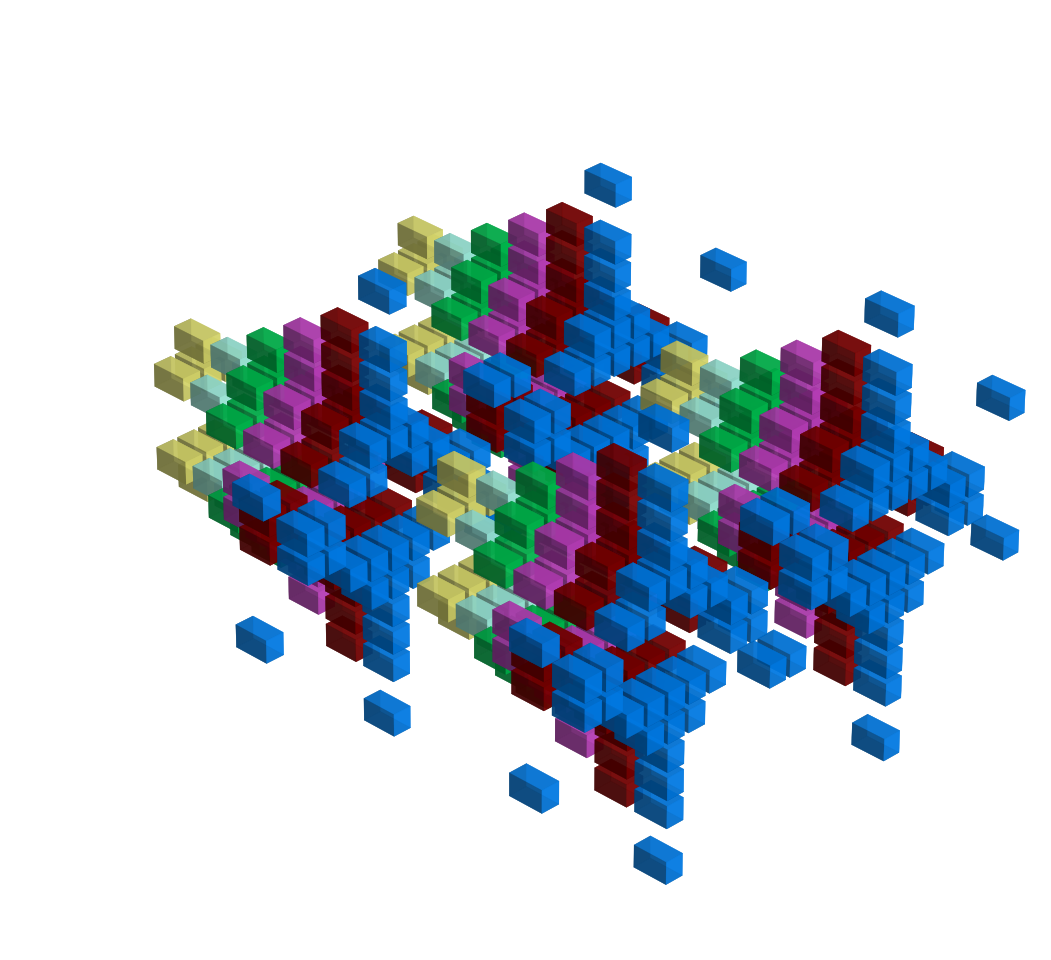
\includegraphics[width=5cm]{src/presets/pattern15-45.png}%           
  \end{adjustbox}                                                        
\caption{Preset 15 come to life.}                                           
\end{figure}                                                               

\clearpage
\begin{minipage}[b]{0.33\linewidth}
\begin{lrbox}{\mybox}%
\begin{lstlisting}[basicstyle=\ttfamily\tiny,escapechar=\%]
burstGeneratorF1%\index{burstGeneratorF1}%
; currentSymmetrySetting%\index{currentSymmetrySetting}%
.BYTE  Y_AXIS_SYMMETRY
; smoothingDelay%\index{smoothingDelay}%
.BYTE $0C
; Burst Position 1
.BYTE $07,$06
; Index to pattern 
.BYTE PULSAR
; Burst Position 2
.BYTE $11,$0D
; Index to pattern 
.BYTE PULSAR
; Burst Position 3
.BYTE $06,$11
; Index to pattern 
.BYTE PULSAR
; Burst Position 4
.BYTE $FF,$0B
; Index to pattern 
.BYTE PULSAR
; Burst Position 5
.BYTE $FF,$00
; Index to pattern 
.BYTE $FF
; Burst Position 6
.BYTE $21,$06
; Index to pattern 
.BYTE $00
; Burst Position 7
.BYTE $06,$01
; Index to pattern 
.BYTE $06
; Burst Position 8
.BYTE $41,$FF
; Index to pattern 
.BYTE $00
; Burst Position 9
.BYTE $06,$01
; Index to pattern 
.BYTE $06
; Burst Position 10
.BYTE $01,$06
; Index to pattern 
.BYTE $00

burstGeneratorF2%\index{burstGeneratorF2}%
; currentSymmetrySetting%\index{currentSymmetrySetting}%
.BYTE Y_AXIS_SYMMETRY
; smoothingDelay%\index{smoothingDelay}%
.BYTE $0C
; Burst Position 1
.BYTE $13,$08
; Index to pattern 
.BYTE STARONE
; Burst Position 2
.BYTE $07,$0F
; Index to pattern 
.BYTE STARONE
; Burst Position 3
.BYTE $FF,$00
; Index to pattern 
.BYTE MULTICROSS
; Burst Position 4
.BYTE $01,$2A
; Index to pattern 
.BYTE $41
; Burst Position 5
.BYTE $02,$00
; Index to pattern 
.BYTE $04
; Burst Position 6
.BYTE $62,$FF
; Index to pattern 
.BYTE $41
; Burst Position 7
.BYTE $06,$40
; Index to pattern 
.BYTE $00
; Burst Position 8
.BYTE $6B,$04
; Index to pattern 
.BYTE $41
; Burst Position 9
.BYTE $FF,$00
; Index to pattern 
.BYTE $FF
; Burst Position 10
.BYTE $00,$FF
; Index to pattern 
.BYTE $00
\end{lstlisting}
\end{lrbox}%
\scalebox{0.8}{\usebox{\mybox}}
\end{minipage}
\begin{minipage}[b]{0.33\linewidth}
\begin{lrbox}{\mybox}%
\begin{lstlisting}[basicstyle=\ttfamily\tiny,escapechar=\%]
burstGeneratorF3%\index{burstGeneratorF3}%
; currentSymmetrySetting%\index{currentSymmetrySetting}%
.BYTE QUAD_SYMMETRY
; smoothingDelay%\index{smoothingDelay}%
.BYTE $01
; Burst Position 1  
.BYTE $08,$01
; Index to pattern 
.BYTE LALLAMITA
; Burst Position 2
.BYTE $FF,$01
; Index to pattern 
.BYTE LALLAMITA
; Burst Position 3
.BYTE $08,$01
; Index to pattern 
.BYTE $02
; Burst Position 4
.BYTE $08,$01
; Index to pattern 
.BYTE $02
; Burst Position 5
.BYTE $08,$01
; Index to pattern 
.BYTE $02
; Burst Position 6
.BYTE $08,$01
; Index to pattern 
.BYTE $02
; Burst Position 7
.BYTE $08,$01
; Index to pattern 
.BYTE $02
; Burst Position 8
.BYTE $FF,$03
; Index to pattern 
.BYTE $02
; Burst Position 9
.BYTE $08,$03
; Index to pattern 
.BYTE $02
; Burst Position 10
.BYTE $08,$03
; Index to pattern 
.BYTE $02

burstGeneratorF4%\index{burstGeneratorF4}%
; currentSymmetrySetting%\index{currentSymmetrySetting}%
.BYTE NO_SYMMETRY
; smoothingDelay%\index{smoothingDelay}%:
.BYTE $11
; Burst Position 1
.BYTE $12,$09
; Index to pattern 
.BYTE CUSTOMPATTERN0
; Burst Position 2
.BYTE $FF,$08
; Index to pattern 
.BYTE STARTWO
; Burst Position 3
.BYTE $02,$08
; Index to pattern 
.BYTE $03
; Burst Position 4
.BYTE $02,$08
; Index to pattern 
.BYTE $03
; Burst Position 5
.BYTE $02,$FF
; Index to pattern 
.BYTE $00
; Burst Position 6
.BYTE $00,$00
; Index to pattern 
.BYTE $00
; Burst Position 7
.BYTE $01,$24
; Index to pattern 
.BYTE $00
; Burst Position 8
.BYTE $05,$01
; Index to pattern 
.BYTE $00
; Burst Position 9 
.BYTE $00,$00
; Index to pattern 
.BYTE $00
; Burst Position 10 
.BYTE $00,$BD
; Index to pattern 
.BYTE $00
\end{lstlisting}
\end{lrbox}%
\scalebox{0.8}{\usebox{\mybox}}
\end{minipage}
\begin{minipage}[b]{0.33\linewidth}
\begin{lrbox}{\mybox}%
\begin{lstlisting}[basicstyle=\ttfamily\tiny,escapechar=\%]
;--------------------
; Unused Data
;--------------------
.BYTE $00,$BD,$00,$B9,$00,$BD,$00,$BD
.BYTE $81,$BD,$81,$FF,$00,$BD,$F1,$FF
.BYTE $00,$28,$81,$FF,$81,$AE,$83,$AE
.BYTE $00,$FF,$81,$EE,$81,$AC,$C1,$BD
.BYTE $C1,$24,$81,$FF,$C1,$FF,$00,$EE
.BYTE $81,$BF,$85,$AE,$81,$EC,$E1,$BF
.BYTE $83,$37,$00,$EE,$81,$BF,$C3,$2E
.BYTE $81,$2E,$00,$FF,$00,$FF,$00,$FD
.BYTE $05,$DC,$02,$EE,$81,$EC,$C7,$0C
.BYTE $00,$68,$81,$EC,$03,$EE,$81,$EE
.BYTE $85,$62,$81,$EE,$01,$EC,$87,$EA
.BYTE $85,$FD,$83,$CD,$42,$EF,$00,$FF
.BYTE $00,$28,$02,$EA,$81,$BD,$85,$BF
.BYTE $81,$FF,$85,$EE,$00,$BF,$87,$BF
.BYTE $00,$EE,$87,$FF,$81,$FF,$A7,$FE
.BYTE $01,$FF,$80,$EE,$FD,$FF,$FF,$FF
\end{lstlisting}
\end{lrbox}%
\scalebox{0.8}{\usebox{\mybox}}
\end{minipage}
\clearpage
\rhead[]{Bursts}
\textbf{Lines 2800-3200.} This is the data used for generating 'bursts', the subject of our chapter
\hyperref[sec:bursts]{\textcolor{blue}{'beatific bursts'}}. 

Only four are defined, each bound to one of the 'Function' keys on the C64\index{C64} keyboard. Each burst consists of
a header specifying the symmetry and smoothing delay used for the burst:
\begin{lstlisting}[escapechar=\%]
; currentSymmetrySetting%\index{currentSymmetrySetting}%
.BYTE NO_SYMMETRY
; smoothingDelay%\index{smoothingDelay}%:
.BYTE $11
\end{lstlisting}

.. followed by a sequence of 'cells' of three bytes each. Each cell gives the X and Y co-ordinates to place a pattern
and a reference to the pattern to draw:
\begin{lstlisting}[escapechar=\%]
; Burst Position 1
.BYTE $12,$09
; Index to pattern 
.BYTE CUSTOMPATTERN0
\end{lstlisting}
\vfill
\begin{figure}[H]
    \centering
    \begin{adjustbox}{width=9cm,center}
      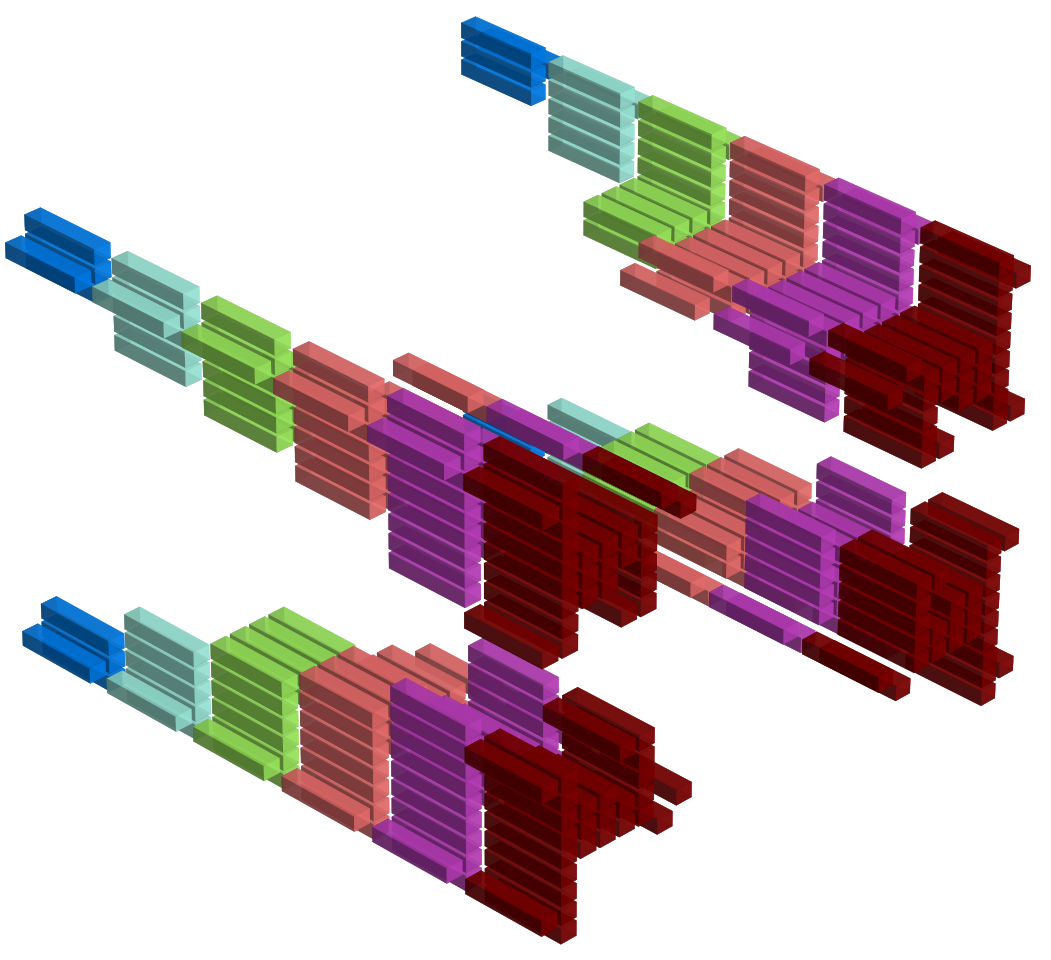
\includegraphics[width=1cm]{src/listing_commentary/diagrams/pattern1-0-45.png}%
      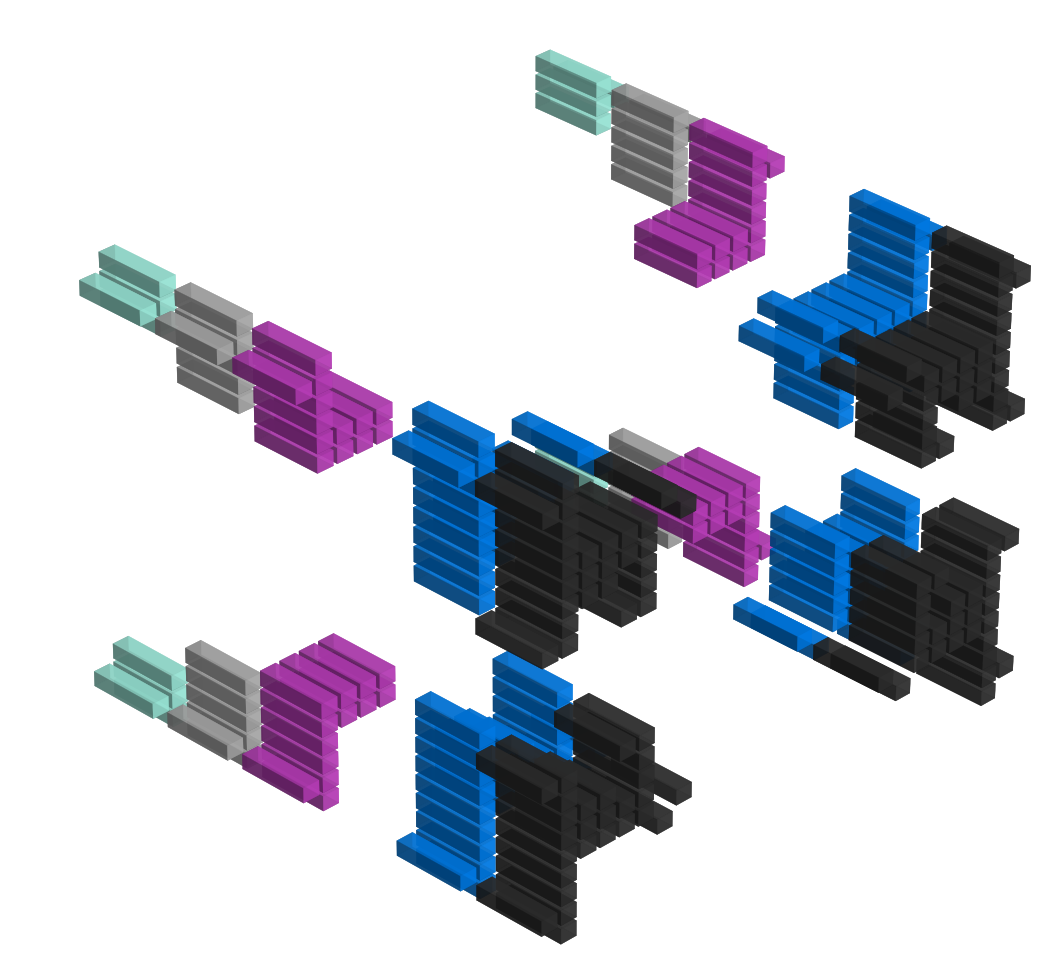
\includegraphics[width=1cm]{src/listing_commentary/diagrams/pattern1-1-45.png}%
    \end{adjustbox}
    \begin{adjustbox}{width=9cm,center}
      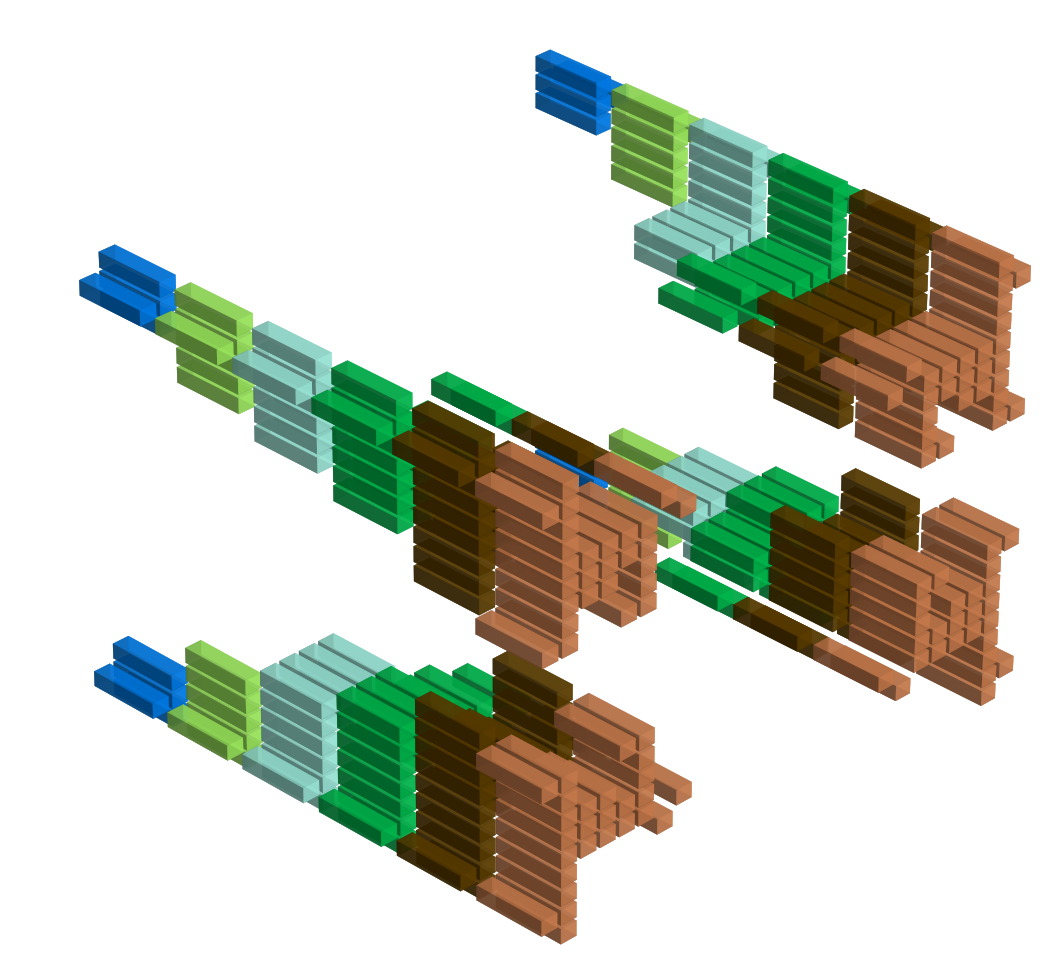
\includegraphics[width=1cm]{src/listing_commentary/diagrams/pattern1-2-45.png}%
      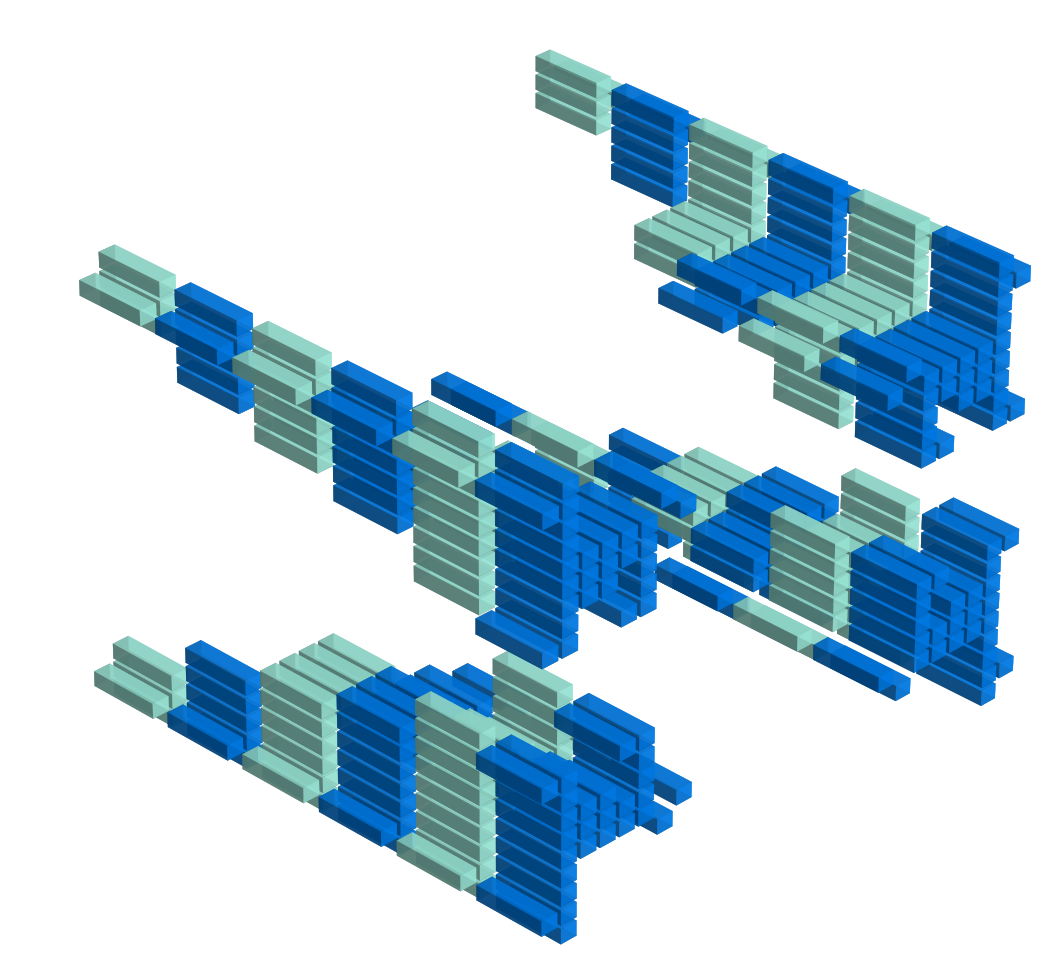
\includegraphics[width=1cm]{src/listing_commentary/diagrams/pattern1-3-45.png}%
    \end{adjustbox}
    \caption{The 'F2' burst in different color schemes}
\end{figure}

\clearpage
\begin{minipage}[b]{0.33\linewidth}
\begin{lrbox}{\mybox}%
\begin{lstlisting}[basicstyle=\ttfamily\tiny,escapechar=\%]
;-----------------------------------
; Sequencer Data
;-----------------------------------
startOfSequencerData = $C300
; currentSymmetrySetting%\index{currentSymmetrySetting}%
.BYTE $01
; smoothingDelay%\index{smoothingDelay}%
.BYTE $0B
; Sequencer Position 1
.BYTE $04,$04  ; X/Y Co-ordinates
.BYTE PULSAR     ; Index to pattern    
; Sequencer Position 2
.BYTE $08,$09  ; X/Y Co-ordinates
.BYTE PULSAR   ; Index to pattern in patternIndexArray%\index{patternIndexArray}%   
; Sequencer Position 3
.BYTE $0C,$0C  ; X/Y Co-ordinates
.BYTE PULSAR   ; Index to pattern
; Sequencer Position 4
.BYTE $10,$11  ; X/Y Co-ordinates
.BYTE PULSAR   ; Index to pattern
; Sequencer Position 5
.BYTE $14,$13  ; X/Y Co-ordinates
.BYTE PULSAR   ; Index to pattern
; Sequencer Position 6
.BYTE $17,$13  ; X/Y Co-ordinates
.BYTE PULSAR   ; Index to pattern
; Each triplet of bytes below
; follows the above pattern.
; The '$FF' below indicates the end of the
; sequencer data.
.BYTE $FF
.BYTE $01,$06,$41,$FF,$00,$06,$01,$06
.BYTE $01,$06,$00,$00,$FF,$06,$00,$02
.BYTE $00,$FF,$41,$46,$00,$06,$81,$AA
.BYTE $41,$02,$00,$04,$62,$FF,$41,$06
.BYTE $40,$00,$6B,$04,$C1,$FF,$00,$FF
.BYTE $00,$FF,$00,$42,$02,$AE,$01,$00
.BYTE $07,$1C,$80,$FF,$05,$06,$01,$02
.BYTE $07,$02,$05,$00,$85,$06,$01,$02
.BYTE $05,$02,$41,$00,$00,$06,$03,$BD
.BYTE $00,$BF,$00,$BF,$C5,$BF,$01,$00
.BYTE $42,$02,$40,$00,$40,$06,$01,$FF
.BYTE $00,$02,$40,$FF,$05,$02,$00,$00
.BYTE $00,$00,$01,$20,$00,$8D,$01,$00
.BYTE $00,$00,$00,$00,$BD,$00,$BD,$00
.BYTE $BD,$40,$BD,$81,$BD,$81,$FF,$00
.BYTE $FF,$F1,$FF,$00,$20,$81,$FF,$81
.BYTE $AE,$C3,$EE,$00,$FF,$81,$EE,$81
.BYTE $AC,$C1,$FD,$D1,$24,$81,$FF,$C1
.BYTE $FF,$00,$AE,$81,$FF,$C5,$EE,$41
.BYTE $EC,$E1,$FF,$C3,$37,$00,$EE,$C1
.BYTE $BF,$C3,$AE,$C1,$AE,$00,$FF,$00
.BYTE $FF,$00,$FD,$05,$DD,$03,$EE,$85
.BYTE $EC,$C7,$4C,$00,$60,$81,$EC,$87
.BYTE $EE,$81,$EE,$8D,$62,$85,$EE,$85
.BYTE $EE,$87,$EA,$85,$FD,$83,$ED,$42
.BYTE $EF,$00,$FF,$40,$28,$02,$EE,$C1
.BYTE $BD,$85,$FF,$81,$FF,$85,$EE,$00
.BYTE $FF,$A7,$BF,$00,$EE,$87,$FF,$81
.BYTE $FF,$A7,$FE,$01,$FF,$00,$EE,$FD
.BYTE $FF,$FF,$FF,$FF,$00,$F7,$00,$FF
.BYTE $00,$BF,$40,$46,$00,$06,$00,$FF
.BYTE $00,$06,$00,$FF,$01,$06,$00,$06
.BYTE $01,$06,$41,$FF,$00,$06,$01,$06
.BYTE $01,$06,$00,$00,$FF,$06,$00,$02
.BYTE $00,$FF,$41,$46,$00,$06,$01,$2A
.BYTE $41,$02,$00,$04,$6A,$FF,$41,$06
.BYTE $40,$00,$4B,$04,$89,$FF,$00,$FF
.BYTE $00,$FF,$00,$42,$02,$BF,$01,$00
.BYTE $07,$1C,$00,$FF,$05,$06,$01,$02
.BYTE $07,$02,$05,$00,$05,$06,$01,$02
.BYTE $05,$02,$01,$00,$00,$06,$02,$BD
.BYTE $00,$BF,$00,$FF,$C5,$BF,$01,$00
.BYTE $42,$02,$40,$00,$40,$06,$01,$FF
.BYTE $00,$02,$40,$FF,$45,$02,$00,$00
.BYTE $00,$02,$01,$24,$00,$05,$01,$00
.BYTE $00,$00,$00,$00,$BD,$00,$B9,$00
.BYTE $BD,$40,$BD,$81,$BD,$81,$FF,$00
.BYTE $FD,$F1,$FF,$00,$20,$81,$FF,$C1
.BYTE $AE,$83,$EE,$00,$FF,$81,$EE,$81
.BYTE $AC,$C1,$BD,$C1,$24,$C1,$FF,$C1
.BYTE $FF,$00,$EE,$81,$FD,$C5,$EE,$C1
.BYTE $EC,$E1,$FF,$C3,$37,$00,$EE,$C1
.BYTE $BF,$C3,$AE,$C1,$AE,$00,$FF,$00
.BYTE $FF,$00,$FD,$81,$DD,$03,$EA,$81
.BYTE $EC,$C7,$CC,$00,$60,$81,$EC,$83
.BYTE $EE,$81,$EE,$85,$62,$81,$EE,$81
.BYTE $EE,$87,$EA,$85,$FD,$83,$ED,$42
.BYTE $EF,$00,$FF,$00,$28,$02,$EE,$81
.BYTE $FD,$85,$FF,$81,$FF,$85,$EE,$00
.BYTE $FD,$85,$FF,$00,$EE,$87,$FF,$81
.BYTE $FF,$A7,$FF,$01,$FF,$80,$EE,$FD
.BYTE $FF,$FF,$FF,$FF,$00,$F7,$00,$FF
.BYTE $00,$BF,$40,$06,$00,$06,$00,$FF
\end{lstlisting}
\end{lrbox}%
\scalebox{0.8}{\usebox{\mybox}}
\end{minipage}
\begin{minipage}[b]{0.33\linewidth}
\begin{lrbox}{\mybox}%
\begin{lstlisting}[basicstyle=\ttfamily\tiny,escapechar=\%]
.BYTE $00,$06,$00,$FF,$21,$06,$00,$06
.BYTE $01,$06,$01,$BF,$00,$06,$01,$06
.BYTE $01,$06,$00,$00,$FF,$06,$00,$02
.BYTE $00,$FF,$41,$46,$00,$06,$01,$2A
.BYTE $01,$02,$00,$04,$62,$FF,$01,$06
.BYTE $40,$00,$6B,$04,$91,$BF,$00,$FF
.BYTE $00,$FF,$00,$42,$02,$BF,$01,$00
.BYTE $07,$1C,$80,$FF,$25,$06,$01,$02
.BYTE $07,$02,$05,$00,$85,$06,$01,$02
.BYTE $05,$02,$01,$00,$00,$06,$03,$BD
.BYTE $00,$BF,$00,$BF,$C5,$BF,$01,$00
.BYTE $42,$02,$40,$00,$00,$06,$01,$FF
.BYTE $00,$02,$40,$FF,$05,$02,$00,$00
.BYTE $00,$00,$01,$20,$00,$8D,$01,$00
.BYTE $00,$00,$00,$00,$BD,$00,$B9,$00
.BYTE $BD,$40,$BD,$81,$BD,$81,$FF,$00
.BYTE $BF,$F9,$FF,$00,$28,$81,$FF,$81
.BYTE $AE,$83,$AE,$00,$FF,$81,$EE,$81
.BYTE $AC,$C1,$BD,$A1,$24,$C1,$FF,$C1
.BYTE $FF,$00,$AE,$81,$BF,$C5,$EE,$C1
.BYTE $EC,$E1,$BF,$83,$3F,$00,$EE,$C1
.BYTE $BF,$E3,$AE,$C1,$AE,$20,$FF,$00
.BYTE $FF,$00,$BD,$05,$DD,$03,$EA,$81
.BYTE $EC,$C7,$4C,$00,$68,$81,$EC,$87
.BYTE $EE,$81,$EE,$AD,$62,$85,$EE,$81
.BYTE $EE,$87,$EA,$85,$FD,$83,$EC,$42
.BYTE $EF,$00,$FF,$00,$28,$02,$EE,$81
.BYTE $BD,$A5,$BF,$81,$BF,$85,$EE,$00
.BYTE $BF,$AF,$BF,$00,$EC,$87,$FF,$81
.BYTE $FF,$A7,$EE,$01,$FF,$80,$EE,$FD
.BYTE $FF,$FF
.BYTE $FF,$FF,$00,$F7,$00,$FF,$00,$BF
.BYTE $40,$46,$00,$06,$00,$FF,$00,$06
.BYTE $00,$FF,$A1,$06,$00,$06,$01,$06
.BYTE $41,$FF,$00,$06,$01,$06,$01,$06
.BYTE $00,$00,$FF,$06,$00,$02,$00,$FF
.BYTE $41,$46,$00,$06,$81,$2A,$01,$02
.BYTE $00,$04,$62,$FF,$41,$06,$40,$00
.BYTE $6B,$04,$B1,$FB,$00,$FF,$00,$FF
.BYTE $00,$42,$02,$B6,$01,$00,$07,$1C
.BYTE $80,$FF,$25,$06,$01,$02,$07,$02
.BYTE $05,$00,$85,$06,$01,$02,$05,$02
.BYTE $01,$00,$00,$06,$03,$BD,$00,$BF
.BYTE $00,$BF,$C5,$BF,$01,$00,$42,$02
.BYTE $40,$00,$40,$06,$01,$FF,$00,$02
.BYTE $40,$FF,$45,$02,$00,$02,$00,$00
.BYTE $01,$A0,$00,$8F,$01,$00,$00,$00
.BYTE $00,$00,$BD,$00,$BD,$00,$BD,$40
.BYTE $BD,$81,$BD,$81,$FF,$00,$FD,$F1
.BYTE $FF,$00,$20,$81,$FF,$81,$AC,$83
.BYTE $EE,$00,$FF,$81,$EE,$81,$AC,$C1
.BYTE $BD,$C1,$24,$C1,$FF,$C1,$FF,$00
.BYTE $EE,$81,$FD,$C5,$AE,$C1,$EC,$E1
.BYTE $BF,$C3,$3F,$00,$EE,$C1,$BF,$C3
.BYTE $AE,$C1,$EE,$00,$FF,$00,$FF,$00
.BYTE $FD,$85,$DD,$03,$EE,$85,$EC,$C7
.BYTE $CC,$00,$E8,$81,$EC,$87,$EE,$81
.BYTE $EE,$8D,$62,$81,$EE,$81,$EE,$87
.BYTE $EA,$85,$FD,$83,$CC,$42,$EF,$00
.BYTE $FF,$00,$28,$02,$EE,$C1,$FD,$85
.BYTE $FF,$81,$FF,$85,$EE,$00,$FD,$85
.BYTE $BF,$00,$EE,$87,$FF,$81,$FF,$87
.BYTE $FE,$01,$FF,$80,$EE,$FD,$FF,$FF
.BYTE $FF,$FF,$00,$F7,$00,$FF,$00,$BF
.BYTE $40,$46,$00,$06,$00,$FF,$00,$06
.BYTE $00,$FF,$11,$06,$00,$06,$01,$06
.BYTE $41,$FF,$00,$06,$01,$06,$01,$06
.BYTE $00,$00,$FF,$06,$00,$02,$00,$FF
.BYTE $41,$46,$00,$06,$01,$AB,$41,$02
.BYTE $00,$04,$62,$FF,$41,$06,$40,$00
.BYTE $6B,$04,$91,$FF,$00,$FF,$00,$FF
.BYTE $00,$42,$02,$27,$01,$00,$07,$1C
.BYTE $00,$FF,$25,$06,$05,$02,$07,$02
.BYTE $05,$00,$05,$06,$01,$02,$05,$02
.BYTE $41,$00,$00,$06,$03,$BD,$00,$BF
.BYTE $00,$BD,$C5,$BF,$01,$00,$42,$02
.BYTE $41,$00,$40,$06,$01,$FF,$00,$02
.BYTE $41,$FF,$45,$02,$00,$00,$00,$00
.BYTE $01,$24,$00,$0D,$01,$00,$00,$00
.BYTE $00,$00,$BD,$00,$FD,$00,$FD,$40
.BYTE $BD,$81,$BD,$81,$FF,$00,$FF,$F1
.BYTE $FF,$00,$20,$81,$FF,$81,$AE,$C3
.BYTE $EE,$00,$FF,$81,$EE,$81,$AC,$C1
.BYTE $FD,$81,$24,$C1,$FF,$C1,$FF,$00
.BYTE $EE,$81,$FF,$C5,$EE,$41,$EC,$E1
.BYTE $FF,$C3,$37,$00,$EE,$C1,$BF,$C3
.BYTE $A6,$C1,$A6,$00,$FF,$00,$FF,$00
.BYTE $BF,$05,$FD,$03,$EA,$85,$EC,$C7
.BYTE $DD,$00,$60,$81,$EC,$87,$EE,$81
.BYTE $EE,$85,$62,$81,$EE,$81,$EE,$87
.BYTE $EA,$85,$FD,$83,$EC,$40,$EF,$00
.BYTE $FF,$00,$28,$02,$EA,$C1,$AC,$85
.BYTE $BF,$81,$FF,$85,$EE,$00,$FF,$C7
.BYTE $BF,$00,$EE,$87,$FF,$81,$FF,$87
.BYTE $FE,$01,$FF,$00,$EE,$FD,$FF,$FF
.BYTE $FF

\end{lstlisting}
\end{lrbox}%
\scalebox{0.8}{\usebox{\mybox}}
\end{minipage}
\clearpage
\rhead[]{Sequencer}
\textbf{Lines 2300-2800.} This data supports Psychedelia's sequencer which we cover in 
\hyperref[sec:sequencer]{\textcolor{blue}{'sensitive sequencer'}}.  Like the burst data it consists of a header, again defining the symmetry and smoothing delay:
\begin{lstlisting}[escapechar=\%]
; currentSymmetrySetting%\index{currentSymmetrySetting}%
.BYTE $01
; smoothingDelay%\index{smoothingDelay}%
.BYTE $0B
\end{lstlisting}

Again like the burst data, the rest of the data consists of cells of three bytes defining X and Y co-ordinates
and a pattern:
\begin{lstlisting}[escapechar=\%]
; Sequencer Position 1
.BYTE $04,$04  ; X/Y Co-ordinates
.BYTE PULSAR     ; Index to pattern    
\end{lstlisting}
\vfill
\begin{figure}[H]
    \centering
    \begin{adjustbox}{width=10cm,center}
      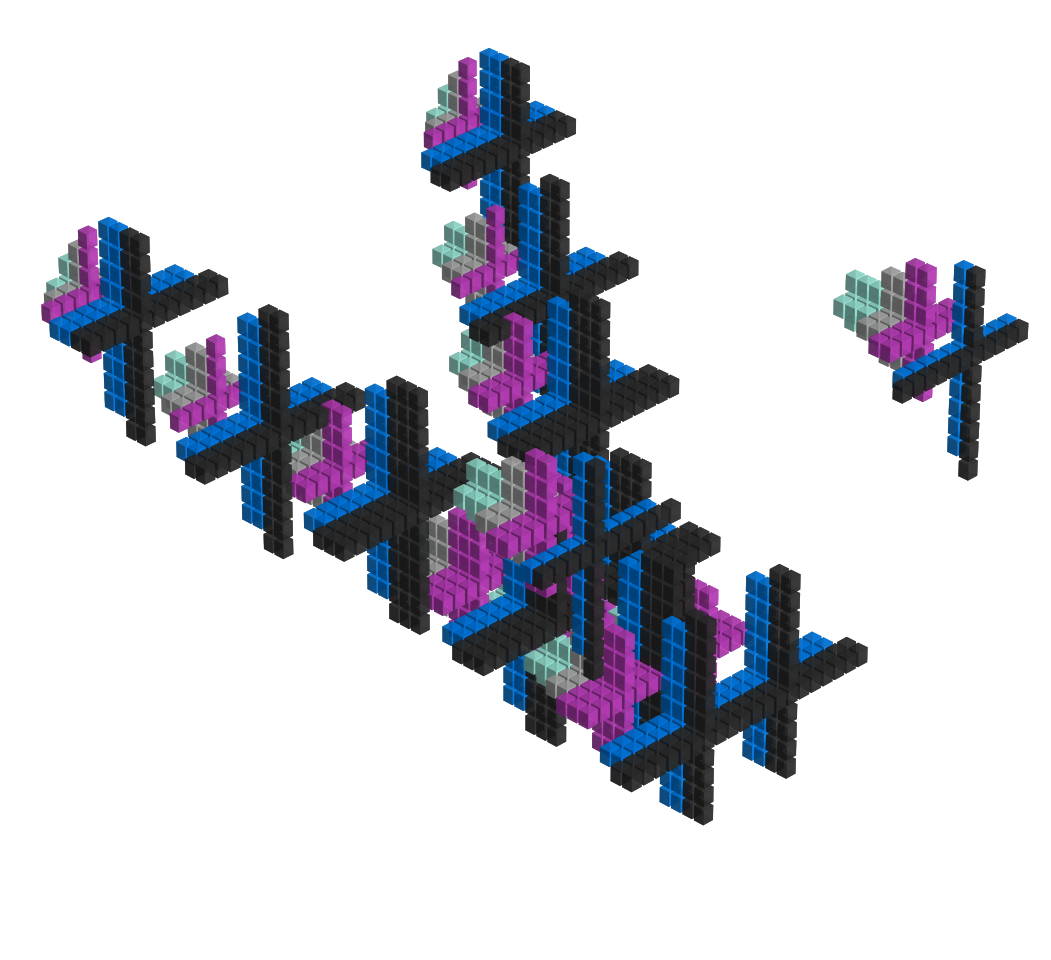
\includegraphics[width=2cm]{src/listing_commentary/sequencer/pattern1-0-45.png}%
      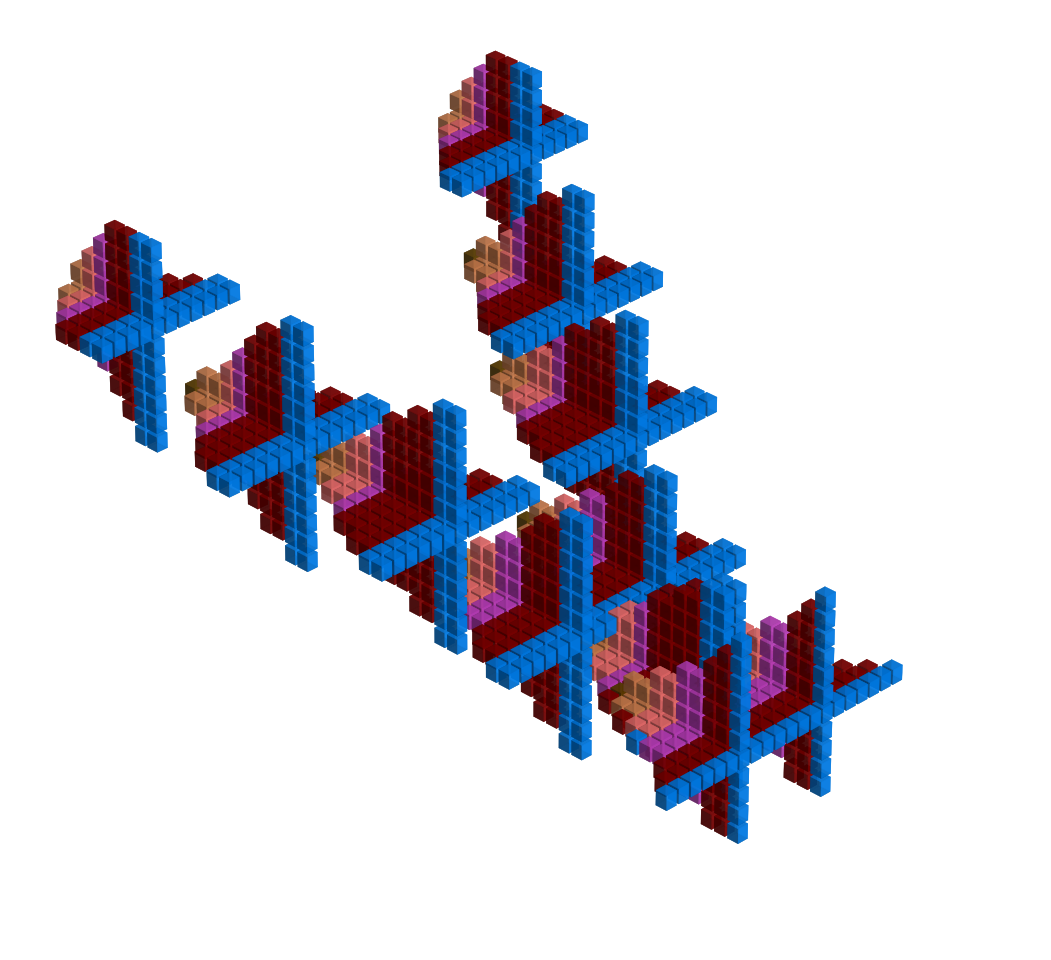
\includegraphics[width=2cm]{src/listing_commentary/sequencer/pattern1-1-45.png}%
    \end{adjustbox}
    \begin{adjustbox}{width=10cm,center}
      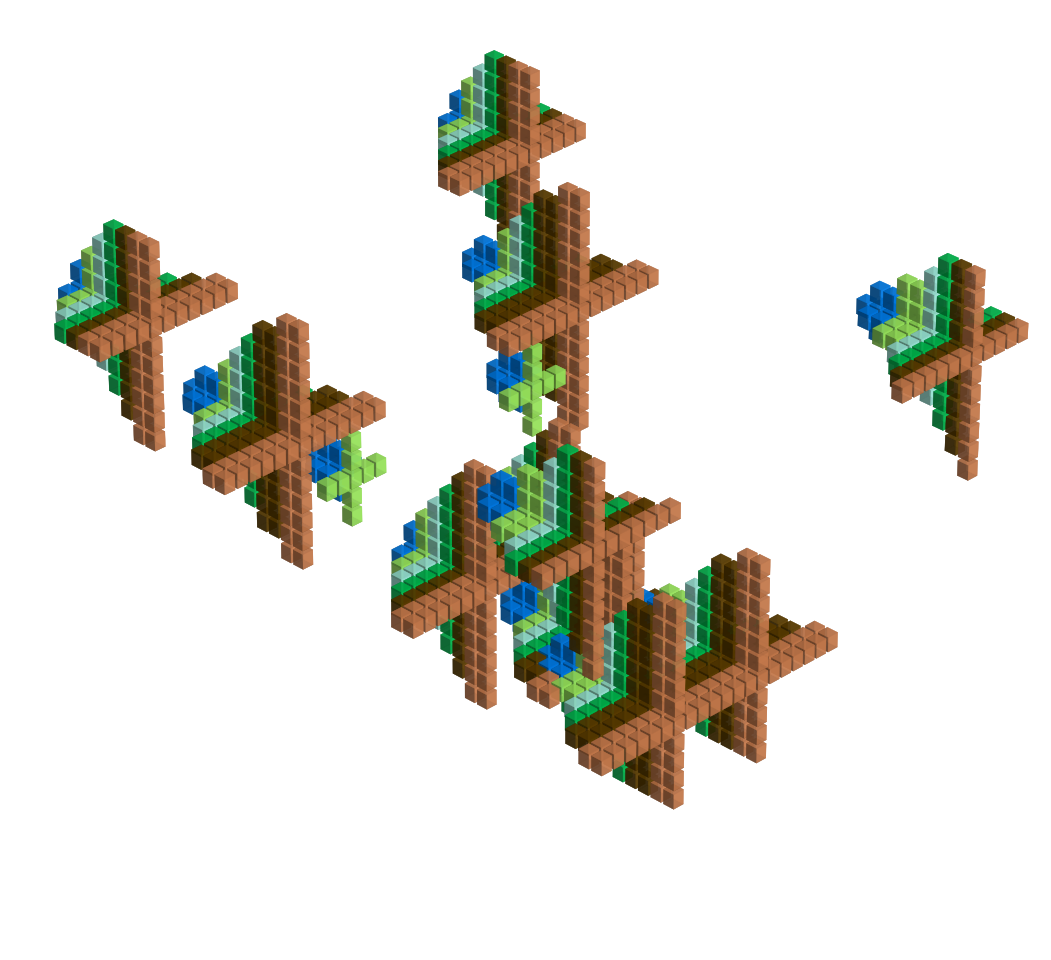
\includegraphics[width=2cm]{src/listing_commentary/sequencer/pattern1-3-45.png}%
      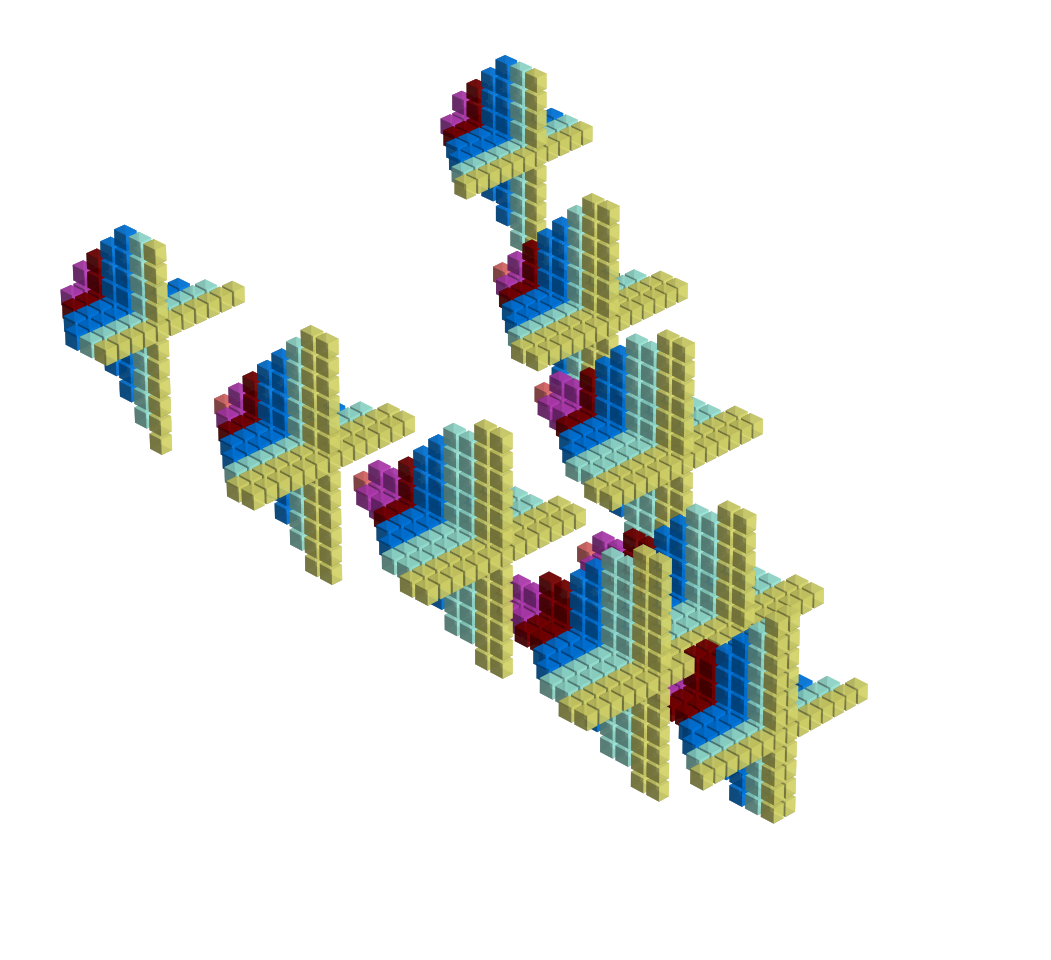
\includegraphics[width=2cm]{src/listing_commentary/sequencer/pattern1-4-45.png}%
    \end{adjustbox}
    \caption{The sequencer in different color schemes}
\end{figure}

\clearpage
\rhead[]{Custom Patterns}
\begin{minipage}[b]{0.33\linewidth}
\begin{lrbox}{\mybox}%
\begin{lstlisting}[basicstyle=\ttfamily\tiny,escapechar=\%]
;
;    33033   
;  35  0  54 
; 5    6    5
; 3   020   4
;    0 2 0   
;  30  2  14 
;    54245   
;
customPattern0XPosArray%\index{customPattern0XPosArray}%
.BYTE $00,$00,$00,$FF,$FE,$FD,$01,$02,$55
.BYTE $00,$03,$55
.BYTE $00,$00,$00,$00,$00,$55
.BYTE $00,$FF,$FE,$FC,$FB,$FC,$01,$02,$55
.BYTE $00,$04,$05,$04,$FF,$01,$55
.BYTE $00,$FD,$FB,$03,$05,$02,$FE,$55
.BYTE $00,$55

.BYTE $00,$00,$00,$00
.BYTE $00,$00,$00,$00,$00,$00,$00,$00
.BYTE $00,$00,$00,$00,$00,$00,$00,$00
.BYTE $00,$00,$00,$00,$00,$00,$00,$00
.BYTE $00,$00,$00,$00,$00,$00,$00,$00
.BYTE $00,$00,$00,$00,$00,$00,$00,$00
.BYTE $00,$00,$00,$00,$00,$00,$00,$00
.BYTE $00,$00,$00,$00,$00,$00,$00,$00
.BYTE $00,$00,$00,$00,$00,$00,$00,$00
.BYTE $00,$00,$00,$00,$00,$00,$00,$00
.BYTE $00,$00,$00,$00,$00,$00,$00,$00

; customPattern0YPosArray%\index{customPattern0YPosArray}%
.BYTE $00,$FF,$FE,$01,$02,$03,$01,$02,$55
.BYTE $00,$03,$55
.BYTE $00,$01,$02,$03,$04,$55
.BYTE $00,$FE,$FE,$FF,$01,$03,$FE,$FE,$55
.BYTE $00,$FF,$01,$03,$04,$04,$55
.BYTE $00,$FF,$00,$FF,$00,$04,$04,$55
.BYTE $00,$55

.BYTE $00,$00,$00,$00
.BYTE $00,$00,$00,$00,$00,$00,$00,$00
.BYTE $00,$00,$00,$00,$00,$00,$00,$00
.BYTE $00,$00,$00,$00,$00,$00,$00,$00
.BYTE $00,$00,$00,$00,$00,$00,$00,$00
.BYTE $00,$00,$00,$00,$00,$00,$00,$00
.BYTE $00,$00,$00,$00,$00,$00,$00,$00
.BYTE $00,$00,$00,$00,$00,$00,$00,$00
.BYTE $00,$00,$00,$00,$00,$00,$00,$00
.BYTE $00,$00,$00,$00,$00,$00,$00,$00
.BYTE $00,$00,$00,$00,$00,$00,$00,$00
;       3      
;    4  5  4   
;       6      
; 3     1     3
;       7      
;     21 12    
;  466     664 
;              
;              
;    3  5  3   
;-----------------
; customPattern1XPosArray%\index{customPattern1XPosArray}%
.BYTE $00,$00,$FF,$01,$55
.BYTE $00,$FE,$02,$55
.BYTE $00,$00,$FA,$06,$03,$FD,$55
.BYTE $00,$FD,$03,$FB,$05,$55
.BYTE $00,$00,$00,$55
.BYTE $00,$00,$FC,$04,$03,$FD,$55
.BYTE $00,$55

.BYTE $00,$00,$00,$00,$00
.BYTE $00,$00,$00,$00,$00,$00,$00,$00
.BYTE $00,$00,$00,$00,$00,$00,$00,$00
.BYTE $00,$00,$00,$00,$00,$00,$00,$00
.BYTE $00,$00,$00,$00,$00,$00,$00,$00
.BYTE $00,$00,$00,$00,$00,$00,$00,$00
.BYTE $00,$00,$00,$00,$00,$00,$00,$00
.BYTE $00,$00,$00,$00,$00,$00,$00,$00
.BYTE $00,$00,$00,$00,$00,$00,$00,$00
.BYTE $00,$00,$00,$00,$00,$00,$00,$00
.BYTE $00,$00,$00,$00,$00,$00,$00,$00
.BYTE $00,$00,$00,$00,$00,$00,$00,$00

; customPattern1YPosArray%\index{customPattern1YPosArray}%
.BYTE $00,$FF,$01,$01,$55
.BYTE $00,$01,$01,$55
.BYTE $00,$FC,$FF,$FF,$05,$05,$55
.BYTE $00,$FD,$FD,$02,$02,$55
.BYTE $00,$05,$FD,$55
.BYTE $00,$FE,$02,$02,$02,$02,$55
.BYTE $00,$55

.BYTE $00,$00,$00,$00,$00
.BYTE $00,$00,$00,$00,$00,$00,$00,$00
.BYTE $00,$00,$00,$00,$00,$00,$00,$00
.BYTE $00,$00,$00,$00,$00,$00,$00,$00
.BYTE $00,$00,$00,$00,$00,$00,$00,$00
.BYTE $00,$00,$00,$00,$00,$00,$00,$00
.BYTE $00,$00,$00,$00,$00,$00,$00,$00
.BYTE $00,$00,$00,$00,$00,$00,$00,$00
.BYTE $00,$00,$00,$00,$00,$00,$00,$00
.BYTE $00,$00,$00,$00,$00,$00,$00,$00
.BYTE $00,$00,$00,$00,$00,$00,$00,$00
.BYTE $00,$00,$00,$00,$00,$00,$00,$00

\end{lstlisting}
\end{lrbox}%
\scalebox{0.8}{\usebox{\mybox}}
\end{minipage}
\begin{minipage}[b]{0.33\linewidth}
\begin{lrbox}{\mybox}%
\begin{lstlisting}[basicstyle=\ttfamily\tiny,escapechar=\%]

;        5       
;      8   8     
;   4         4  
;                
;                
; 3   2  9  2   3
;                
;                
;        6       
;-----------------
customPattern2XPosArray%\index{customPattern2XPosArray}%
.BYTE $00,$55
.BYTE $00,$FD,$03,$55
.BYTE $00,$F9,$07,$55
.BYTE $00,$FB,$05,$55
.BYTE $00,$00,$55
.BYTE $00,$00,$55
.BYTE $00,$55
.BYTE $FE,$02,$55
.BYTE $00,$55
.BYTE $55

.BYTE $00,$00,$00,$00
.BYTE $00,$00,$00,$00,$00,$00,$00,$00
.BYTE $00,$00,$00,$00,$00,$00,$00,$00
.BYTE $00,$00,$00,$00,$00,$00,$00,$00
.BYTE $00,$00,$00,$00,$00,$00,$00,$00
.BYTE $00,$00,$00,$00,$00,$00,$00,$00
.BYTE $00,$00,$00,$00,$00,$00,$00,$00
.BYTE $00,$00,$00,$00,$00,$00,$00,$00
.BYTE $00,$00,$00,$00,$00,$00,$00,$00
.BYTE $00,$00,$00,$00,$00,$00,$00,$00

; customPattern2YPosArray%\index{customPattern2YPosArray}%
.BYTE $00,$55
.BYTE $00,$00,$00,$55
.BYTE $00,$00,$00,$55
.BYTE $00,$FD,$FD,$55
.BYTE $00,$FB,$55
.BYTE $00,$04,$55
.BYTE $00,$55
.BYTE $FC,$FC,$55
.BYTE $00,$55
.BYTE $55
.BYTE $00,$00,$00,$00
.BYTE $00,$00,$00,$00,$00,$00,$00,$00
.BYTE $00,$00,$00,$00,$00,$00,$00,$00
.BYTE $00,$00,$00,$00,$00,$00,$00,$00
.BYTE $00,$00,$00,$00,$00,$00,$00,$00
.BYTE $00,$00,$00,$00,$00,$00,$00,$00
.BYTE $00,$00,$00,$00,$00,$00,$00,$00
.BYTE $00,$00,$00,$00,$00,$00,$00,$00
.BYTE $00,$00,$00,$00,$00,$00,$00,$00
.BYTE $00,$00,$00,$00,$00,$00,$00,$00
.BYTE $00,$00,$00,$00,$00,$00,$00,$00
.BYTE $00,$00,$00,$00,$00,$00,$00,$00

;  5    
; 66  1 
;  4 711
;   4222
;    3 2
;    3 3
;-----------------
; customPattern3XPosArray%\index{customPattern3XPosArray}%
.BYTE $00,$01,$01,$02,$55
.BYTE $00,$00,$01,$02,$02,$55
.BYTE $00,$00,$00,$02,$55
.BYTE $00,$FF,$FE,$55
.BYTE $00,$FE,$FE,$55
.BYTE $00,$FD,$FE,$55
.BYTE $00,$55

.BYTE $00,$00
.BYTE $00,$00,$00,$00,$00,$00,$00,$00
.BYTE $00,$00,$00,$00,$00,$00,$00,$00
.BYTE $00,$00,$00,$00,$00,$00,$00,$00
.BYTE $00,$00,$00,$00,$00,$00,$00,$00
.BYTE $00,$00,$00,$00,$00,$00,$00,$00
.BYTE $00,$00,$00,$00,$00,$00,$00,$00
.BYTE $00,$00,$00,$00,$00,$00,$00,$00
.BYTE $00,$00,$00,$00,$00,$00,$00,$00
.BYTE $00,$00,$00,$00,$00,$00,$00,$00
.BYTE $00,$00,$00,$00,$00,$00,$00,$00
.BYTE $00,$00,$00,$00,$00,$00,$00,$00

; customPattern3YPosArray%\index{customPattern3YPosArray}%
.BYTE $00,$FF,$00,$00,$55
.BYTE $00,$01,$01,$01,$02,$55
.BYTE $00,$02,$03,$03,$55
.BYTE $00,$01,$00,$55
.BYTE $00,$FF,$FE,$55
.BYTE $00,$FF,$FF,$55
.BYTE $00,$55

.BYTE $00,$00
.BYTE $00,$00,$00,$00,$00,$00,$00,$00
.BYTE $00,$00,$00,$00,$00,$00,$00,$00
.BYTE $00,$00,$00,$00,$00,$00,$00,$00
.BYTE $00,$00,$00,$00,$00,$00,$00,$00
.BYTE $00,$00,$00,$00,$00,$00,$00,$00
.BYTE $00,$00,$00,$00,$00,$00,$00,$00
.BYTE $00,$00,$00,$00,$00,$00,$00,$00
.BYTE $00,$00,$00,$00,$00,$00,$00,$00
.BYTE $00,$00,$00,$00,$00,$00,$00,$00
.BYTE $00,$00,$00,$00,$00,$00,$00,$00
.BYTE $00,$00,$00,$00,$00,$00,$00,$00
\end{lstlisting}
\end{lrbox}%
\scalebox{0.8}{\usebox{\mybox}}
\end{minipage}
\begin{minipage}[b]{0.33\linewidth}
\begin{lrbox}{\mybox}%
\begin{lstlisting}[basicstyle=\ttfamily\tiny,escapechar=\%]



;                1                    
;                                     
;                                     
;                                     
;                                     
;                3                    
;                                     
;                                     
;                4                    
;                                     
;                5                    
;                6                    
; 1    2     99 6106899      2    1
;                                     
;                                     
;                                     
;                                     
;                                     
;                                     
;                                     
;                                     
;                                     
;                                     
;                1                    
; customPattern4XPosArray%\index{customPattern4XPosArray}%
.BYTE $00,$00,$00,$ED,$14,$55
.BYTE $00,$F2,$0F,$55
.BYTE $00,$00,$55
.BYTE $00,$00,$55
.BYTE $00,$00,$55
.BYTE $00,$00,$FF,$01,$55
.BYTE $00,$55
.BYTE $02,$55
.BYTE $00,$FC,$FD,$03,$04,$55
.BYTE $00,$55

.BYTE $00,$00,$00,$00
.BYTE $00,$00,$00,$00,$00,$00,$00,$00
.BYTE $00,$00,$00,$00,$00,$00,$00,$00
.BYTE $00,$00,$00,$00,$00,$00,$00,$00
.BYTE $00,$00,$00,$00,$00,$00,$00,$00
.BYTE $00,$00,$00,$00,$00,$00,$00,$00
.BYTE $00,$00,$00,$00,$00,$00,$00,$00
.BYTE $00,$00,$00,$00,$00,$00,$00,$00
.BYTE $00,$00,$00,$00,$00,$00,$00,$00
.BYTE $00,$00,$00,$00,$00,$00,$00,$00
.BYTE $00,$00,$00,$00,$00,$00,$00,$00
.BYTE $00,$00,$00,$00,$00,$00,$00,$00

; customPattern4YPosArray%\index{customPattern4YPosArray}%
.BYTE $00,$0B,$F4,$00,$00,$55
.BYTE $00,$00,$00,$55
.BYTE $00,$F9,$55
.BYTE $00,$FC,$55
.BYTE $00,$FE,$55
.BYTE $00,$FF,$00,$00,$55
.BYTE $00,$55
.BYTE $00,$55
.BYTE $00,$00,$00,$00,$00,$55
.BYTE $00,$55

.BYTE $00,$00,$00,$00
.BYTE $00,$00,$00,$00,$00,$00,$00,$00
.BYTE $00,$00,$00,$00,$00,$00,$00,$00
.BYTE $00,$00,$00,$00,$00,$00,$00,$00
.BYTE $00,$00,$00,$00,$00,$00,$00,$00
.BYTE $00,$00,$00,$00,$00,$00,$00,$00
.BYTE $00,$00,$00,$00,$00,$00,$00,$00
.BYTE $00,$00,$00,$00,$00,$00,$00,$00
.BYTE $00,$00,$00,$00,$00,$00,$00,$00
.BYTE $00,$00,$00,$00,$00,$00,$00,$00
.BYTE $00,$00,$00,$00,$00,$00,$00,$00
.BYTE $00,$00,$00,$00,$00,$00,$00,$00






























;
\end{lstlisting}
\end{lrbox}%
\scalebox{0.8}{\usebox{\mybox}}
\end{minipage}
\textbf{Lines 2800-3200.} The final batch of data at the very end of the program consists of the
eight 'custom patterns', programmable by the player.

Likely as not these were the last feature to be implemented. They are after all appended to the very
end of the code base. We cover these, along with all the other patterns, in our next chapter. 

One feature worth noting here is the large number of zero bytes added as padding at the end of each 
definition. At first glance, this seems curious and wasteful. The explanation is one of simple convenience:
padding the data structure this way ensures that the \icode{*XPosArray} and \icode{*YPosArray} definitions occur at memory
addresses that are a multiple of \icode{\$80}. For example, \icode{\$2D00, \$2D80, \$2E00} and so on.
This means that, when referencing, the programmer just
has to increment their position in memory by \icode{\$80} bytes each to move to and fetch the next array.

Now that we've had a good look at the overall layout of Psychedelia's code - let's bury our head in some gory detail
and some pretty pictures.
\vfill


\begin{minipage}[b]{1\linewidth}
\begin{minipage}[b]{0.33\linewidth}
\begin{lrbox}{\mybox}%
\begin{lstlisting}[basicstyle=\ttfamily\tiny,escapechar=\%]
;-----------------

;   44455566
;       1   
;       1   
;      1    
;      7    
;     2     
;     2     
; 3  2      
;  33       
;-----------------
; customPattern5XPosArray%\index{customPattern5XPosArray}%
.BYTE $00,$00,$01,$01,$55
.BYTE $00,$FF,$FF,$FE,$55
.BYTE $00,$FD,$FC,$FB,$55
.BYTE $00,$FD,$FE,$FF,$55
.BYTE $00,$00,$01,$02,$55
.BYTE $00,$03,$04,$55
.BYTE $00,$55

.BYTE $00
.BYTE $00,$00,$00,$00,$00,$00,$00,$00
.BYTE $00,$00,$00,$00,$00,$00,$00,$00
.BYTE $00,$00,$00,$00,$00,$00,$00,$00
.BYTE $00,$00,$00,$00,$00,$00,$00,$00
.BYTE $00,$00,$00,$00,$00,$00,$00,$00
.BYTE $00,$00,$00,$00,$00,$00,$00,$00
.BYTE $00,$00,$00,$00,$00,$00,$00,$00
.BYTE $00,$00,$00,$00,$00,$00,$00,$00
.BYTE $00,$00,$00,$00,$00,$00,$00,$00
.BYTE $00,$00,$00,$00,$00,$00,$00,$00
.BYTE $00,$00,$00,$00,$00,$00,$00,$00
.BYTE $00,$00,$00,$00,$00,$00,$00,$00

; customPattern5YPosArray%\index{customPattern5YPosArray}%
.BYTE $00,$FF,$FE,$FD,$55
.BYTE $00,$01,$02,$03,$55
.BYTE $00,$04,$04,$03,$55
.BYTE $00,$FC,$FC,$FC,$55
.BYTE $00,$FC,$FC,$FC,$55
.BYTE $00,$FC,$FC,$55
.BYTE $00,$55



.BYTE $00
.BYTE $00,$00,$00,$00,$00,$00,$00,$00
.BYTE $00,$00,$00,$00,$00,$00,$00,$00
.BYTE $00,$00,$00,$00,$00,$00,$00,$00
.BYTE $00,$00,$00,$00,$00,$00,$00,$00
.BYTE $00,$00,$00,$00,$00,$00,$00,$00
.BYTE $00,$00,$00,$00,$00,$00,$00,$00
.BYTE $00,$00,$00,$00,$00,$00,$00,$00
.BYTE $00,$00,$00,$00,$00,$00,$00,$00
.BYTE $00,$00,$00,$00,$00,$00,$00,$00
.BYTE $00,$00,$00,$00,$00,$00,$00,$00
.BYTE $00,$00,$00,$00,$00,$00,$00,$00
.BYTE $00,$00,$00,$00,$00,$00,$00,$00


\end{lstlisting}
\end{lrbox}%
\scalebox{0.8}{\usebox{\mybox}}
\end{minipage}
\begin{minipage}[b]{0.33\linewidth}
\begin{lrbox}{\mybox}%
\begin{lstlisting}[basicstyle=\ttfamily\tiny,escapechar=\%]
;      3            
;     3 3           
; 2    3            
; 2                 
;             1     
;            1      
;           8       
;    6              
;                  5
;  6   6         5  
;                   
;        44         
;        44         
;-----------------
; customPattern6XPosArray%\index{customPattern6XPosArray}%
.BYTE $00,$01,$02,$55
.BYTE $00,$F6,$F6,$55
.BYTE $00,$FB,$FA,$FB,$FC,$55
.BYTE $00,$FD,$FD,$FE,$FE,$55
.BYTE $00,$05,$07,$55
.BYTE $00,$F9,$F7,$FB,$55
.BYTE $00,$55
.BYTE $00,$55

.BYTE $00,$00,$00,$00,$00,$00,$00
.BYTE $00,$00,$00,$00,$00,$00,$00,$00
.BYTE $00,$00,$00,$00,$00,$00,$00,$00
.BYTE $00,$00,$00,$00,$00,$00,$00,$00
.BYTE $00,$00,$00,$00,$00,$00,$00,$00
.BYTE $00,$00,$00,$00,$00,$00,$00,$00
.BYTE $00,$00,$00,$00,$00,$00,$00,$00
.BYTE $00,$00,$00,$00,$00,$00,$00,$00
.BYTE $00,$00,$00,$00,$00,$00,$00,$00
.BYTE $00,$00,$00,$00,$00,$00,$00,$00
.BYTE $00,$00,$00,$00,$00,$00,$00,$00
.BYTE $00,$00,$00,$00,$00,$00,$00,$00

; customPattern6YPosArray%\index{customPattern6YPosArray}%
.BYTE $00,$FF,$FE,$55
.BYTE $00,$FC,$FD,$55
.BYTE $00,$FA,$FB,$FC,$FB,$55
.BYTE $00,$05,$06,$06,$05,$55
.BYTE $00,$03,$02,$55
.BYTE $00,$01,$03,$03,$55
.BYTE $00,$55
.BYTE $00,$55

.BYTE $00,$00,$00,$00,$00,$00,$00
.BYTE $00,$00,$00,$00,$00,$00,$00,$00
.BYTE $00,$00,$00,$00,$00,$00,$00,$00
.BYTE $00,$00,$00,$00,$00,$00,$00,$00
.BYTE $00,$00,$00,$00,$00,$00,$00,$00
.BYTE $00,$00,$00,$00,$00,$00,$00,$00
.BYTE $00,$00,$00,$00,$00,$00,$00,$00
.BYTE $00,$00,$00,$00,$00,$00,$00,$00
.BYTE $00,$00,$00,$00,$00,$00,$00,$00
.BYTE $00,$00,$00,$00,$00,$00,$00,$00
.BYTE $00,$00,$00,$00,$00,$00,$00,$00
.BYTE $00,$00,$00,$00,$00,$00,$00,$00
\end{lstlisting}
\end{lrbox}%
\scalebox{0.8}{\usebox{\mybox}}
\end{minipage}
\begin{minipage}[b]{0.33\linewidth}
\begin{lrbox}{\mybox}%
\begin{lstlisting}[basicstyle=\ttfamily\tiny,escapechar=\%]
;
;
;
;
;
;
;
; customPattern7XPosArray%\index{customPattern7XPosArray}%
.BYTE $00,$55
.BYTE $00,$55
.BYTE $00,$55
.BYTE $00,$55
.BYTE $00,$55
.BYTE $00,$55
.BYTE $00,$55

.BYTE $00,$00
.BYTE $00,$00,$00,$00,$00,$00,$00,$00
.BYTE $00,$00,$00,$00,$00,$00,$00,$00
.BYTE $00,$00,$00,$00,$00,$00,$00,$00
.BYTE $00,$00,$00,$00,$00,$00,$00,$00
.BYTE $00,$00,$00,$00,$00,$00,$00,$00
.BYTE $00,$00,$00,$00,$00,$00,$00,$00
.BYTE $00,$00,$00,$00,$00,$00,$00,$00
.BYTE $00,$00,$00,$00,$00,$00,$00,$00
.BYTE $00,$00,$00,$00,$00,$00,$00,$00
.BYTE $00,$00,$00,$00,$00,$00,$00,$00
.BYTE $00,$00,$00,$00,$00,$00,$00,$00
.BYTE $00,$00,$00,$00,$00,$00,$00,$00
.BYTE $00,$00,$00,$00,$00,$00,$00,$00
.BYTE $00,$00,$00,$00,$00,$00,$00,$00

; customPattern7YPosArray%\index{customPattern7YPosArray}%
.BYTE $00,$55
.BYTE $00,$55
.BYTE $00,$55
.BYTE $00,$55
.BYTE $00,$55
.BYTE $00,$55
.BYTE $00,$55

.BYTE $00,$00
.BYTE $00,$00,$00,$00,$00,$00,$00,$00
.BYTE $00,$00,$00,$00,$00,$00,$00,$00
.BYTE $00,$00,$00,$00,$00,$00,$00,$00
.BYTE $00,$00,$00,$00,$00,$00,$00,$00
.BYTE $00,$00,$00,$00,$00,$00,$00,$00
.BYTE $00,$00,$00,$00,$00,$00,$00,$00
.BYTE $00,$00,$00,$00,$00,$00,$00,$00
.BYTE $00,$00,$00,$00,$00,$00,$00,$00
.BYTE $00,$00,$00,$00,$00,$00,$00,$00
.BYTE $00,$00,$00,$00,$00,$00,$00,$00
.BYTE $00,$00,$00,$00,$00,$00,$00,$00
.BYTE $00,$00,$00,$00,$00,$00,$00,$00
.BYTE $00,$00,$00,$00,$00,$00,$00,$00
.BYTE $00,$00,$00,$00,$00,$00,$00
.BYTE $FF
dynamicStorage%\index{dynamicStorage}%
.BYTE $00
\end{lstlisting}
\end{lrbox}%
\scalebox{0.8}{\usebox{\mybox}}
\end{minipage}
\end{minipage}
